\chapter{Investigating the Molecular Mechanisms of Tension-dependent Re-localisation of Shugoshin}

\section{Introduction}
Centromere executes its function of coordinating chromosome segregation partially by controlling the subcellular location of critical regulators. A remarkable example is the tension-dependent re-localisation of shugoshin. 

To be segregated into different daughter cells later, sister chromatids need to be bipolarly attached to the spindle in mitosis or meiosis II, which is called bi-orientation \citep{Tanaka2010Kinetochore-microtubuleBi-orientation}. Bi-oriented sister chromatids come under tension due to the counteraction between the resistance of cohesion and the pulling of microtubules. Cells sense a lack of tension and destabilise erroneous microtubule-kinetochore attachment, a process termed error correction, meanwhile delaying cell cycle progression until tension is generated \citep{Nicklas1997HowChromosomes, Nicklas1994, Tanaka2010Kinetochore-microtubuleBi-orientation}. The conserved shugoshin protein family is important for the establishment of tension \citep{Watanabe2005, Clift2011, Gutierrez-Caballero2012Shugoshins:Centromere, Marston2015, Zhang2020FunctioningMitosis}. The name itself, 'guardian spirit' in Japanese, comes from its well-conserved canonical function of cohesion protection in meiosis I \citep{Lister2010Age-relatedSgo2, Llano2008Shugoshin-2Mice, Lee2008, Rattani2013Sgol2Oocytes, Marston2004a, Kitajima2004a, Katis2004, Rabitsch2004TwoII, Kerrebrock1992TheDifferentiation, Cromer2013CentromericInterkinesis, Zamariola2014SHUGOSHINsThaliana, Wang2011OsSGO1Meiosis, Hamant2005AFunctions, Ma2021MeikinI, Miyazaki2017HierarchicalI}. In vertebrates, shugoshin also protects centromeric cohesion from Wapl-mediated cohesin removal pathway in mitosis \citep{Rivera2009ShugoshinExtracts, Shintomi2009ReleasingSgo1, Huang2007, Tang2006a, McGuinness2005ShugoshinCells, Kitajima2005, Salic2004VertebrateMitosis, Liang2019ACells}. Shugoshin further assists cohesion protection by directly sequestering separase with the SAC component Mad2 \citep{Rattani2013Sgol2Oocytes, Hellmuth2020Securin-independentShugoshinMAD2, Orth2011ShugoshinMad2}. Apart from cohesion protection, shugoshin additionally promotes bi-orientation by facilitating error correction \citep{Meppelink2015Shugoshin-1Bi-orientation, Huang2007, Peplowska2014, Nerusheva2014, Verzijlbergen2014, Tsukahara2010a, Yamagishi2010, Hadders2020UntanglingMitosis, Broad2020AuroraCells, Kawashima2007, Vanoosthuyse2007, Rivera2012} and, at least in yeast, contributing to the geometry of the centromeric region biased towards a shape where sister kinetochores are more easily captured by microtubules from the opposite spindle poles \citep{Indjeian2007, Haase2012Bub1Dynamics, Verzijlbergen2014, Peplowska2014, Sane2021ShugoshinDisassembly}. Despite different molecular details in various species, all these functions are implemented by shugoshin acting as an adaptor recruiting different effector proteins to the centromeric region, including PP2A-B' \citep{Xu2009StructureInteraction, Ueki2021AMitosis}, CPC \citep{Abad2022MechanisticCPC}, MCAK \citep{Tanno2010} and condensin \citep{Verzijlbergen2014, Yahya2020}. 

Interestingly, the location of shugoshin has been found to change in response to tension across species. Human Sgo1 and Sgo2 redistribute from the inner centromere towards the kinetochore upon tension establishment in mitosis \citep{Huang2007, Lee2008, Liu2013, Asai2020}. Mouse Sgo2 follows the same pattern in meiosis II \citep{Lee2008, Gomez2007}. In budding yeast, tension removes its only shugoshin protein Sgo1 from peri-centromere \citep{Eshleman2014, Nerusheva2014, Paldi2020ConvergentPericentromeres}. Although the effect of tension has not been directly studied, locations are different between metaphase and anaphase for \textit{Drosophila} MEI-S332 (mitosis and meiosis II) and fission yeast Sgo2 (mitosis) \citep{Clarke2005, Kawashima2007}, raising the possibility that they also undergo tension-dependent re-localisation. 

Re-localisation of shugoshin is functionally relevant. It has been proposed as key to tension sensing \citep{Marston2015}. Screening in budding yeast identified Sgo1 being required to delay anaphase onset in the absence of tension \citep{Indjeian2005a}. Later, it was shown to be due to its role in preventing SAC silencing \citep{Jin2013TheAttachment}. Given the function of Sgo1 to support CPC localisation, it was reasoned that tension-dependent re-localisation of Sgo1 triggers the removal of CPC from the centromere, leading to SAC silencing \citep{Nerusheva2014}. In support of this model, artificially tethering Sgo1 to the kinetochore caused prolonged metaphase \citep{Su2021SumoylationAnaphase}. In mammals, the re-localisation is thought to inactivate cohesin protection \citep{Lee2008}. Indeed, impaired human Sgo1 re-localisation increased lagging chromosomes in anaphase \citep{Liu2013}. Besides, at least in budding yeast, the re-localisation of shugoshin might be the signal for chromosome condensation. The key condensation player condensin spreads from the centromere to chromosome arms in a tension-dependent manner \citep{Leonard2015}. As its interactor with a similar response to tension, Sgo1 potentially mediates the spread. Consistent with this idea, mitotic chromosome condensation is abolished in \textit{sgo1} mutant \citep{Kruitwagen2018}. 

It is well established across species that the SAC component Bub1 kinase at the kinetochore phosphorylates threonine 120 of histone H2A (serine 121 in yeast) around centromeric chromatin, providing a high-affinity marker for shugoshin \citep{Rivera2012, Boyarchuk2007Bub1Centromere, Williams2017Bub1Kinetochores, Kitajima2005, Perera2010, Tang2004, Fernius2007Bub1Mitosis, Kiburz2005, Kawashima2010a}. Nevertheless, the localisation of shugoshin is further regulated by complicated, not fully understood, interplay of various factors through reversible PTMs. In human cells, a step-wise recruitment model of Sgo1 has been proposed \citep{Liu2013, Liu2013a, Liu2015}. Sgo1 is first recruited proximal to the kinetochore due to direct binding to nucleosomes with H2A-pT120. Pol II-mediated centromeric transcription then disengages Sgo1 from nucleosomes, allowing it to reach the inner centromere. Finally, Sgo1 phosphorylated at threonine 346 by CDK is captured by cohesin there. A number of other factors supporting shugoshin localisation have been reported in different species, including HP1 \citep{Yamagishi2008, Kang2011, Perera2010}, CPC \citep{Huang2007, Tanno2010, Rivera2012, Kawashima2007, Boyarchuk2007Bub1Centromere, Resnick2006INCENPDrosophila}, PP2A \citep{Tang2006a}, CENP-A \citep{Petty2018ConnectingCheckpoint, Eot-Houllier2018AuroraFatigue, Mishra2018BuddingChromatin} and H3 \citep{Buehl2018a, Luo2016}, while Polo kinase \citep{Clarke2005}, SET \citep{Qu2019SETSegregation, Krishnan2017Phospho-H1Mitosis}, KAT2A \citep{Petty2018ConnectingCheckpoint} and PP2A \citep{Nerusheva2014} were suggested to de-localise it. 

The mechanism of shugoshin tension-dependent re-localisation is less well understood. \cite{Nerusheva2014} attempted to address it in budding yeast, yet questions are left to be answered. It was proposed that reduced Bub1 activity at peri-centromere by tension leads to the de-phosphorylation of its substrate(s), thus resulting in the removal of Sgo1 (Figure~\ref{fig:naive}). How Bub1 activity in a particular area is regulated by tension remains to be elucidated. Due to technical difficulties, it was unable to directly monitor H2A-pS121 by that time, leaving the effect of tension on it untested. Moreover, this model predicts the existence of at least one phosphatase antagonizing Bub1. Although it was found that PP2A-B' (Rts1 in budding yeast) negatively regulates Sgo1 enrichment at the peri-centromere, whether it is responsible for Sgo1 de-localisation is unclear. The human model emphasizes phospho-regulation of shugoshin interaction with cohesin by tension underlying its movement from the inner centromere to the kinetochore-proximal region \citep{Liu2013, Liu2015}. It is interesting to explore if this mechanism could be conserved in budding yeast as well. Besides, the exact localisation of human H2A-pT120 by IF is inconsistent in the literature, with reports arguing it covers both the inner centromere \citep{Yamagishi2010} and the kinetochore proximity or it is usually only at the latter \citep{Liu2013}. Due to the repetitive nature of human centromere, the two arguments could not be distinguished by sequence-based technology such as ChIP. Whereas budding yeast can be used to address this question for its point centromere structure. 

\begin{figure}[htbp]
  \centering
  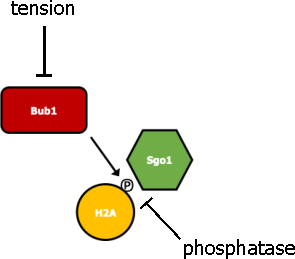
\includegraphics[width=0.3\textwidth]{figures/naive model.pdf}
  \caption[Proposed budding yeast model of tension-dependent re-localisation of Sgo1]{Proposed budding yeast model of tension-dependent re-localisation of Sgo1. Tension causes a reduction of Bub1 phosphorylation capability at peri-centromere, resulting in the de-phosphorylation of the substrates (H2A-S121 is used as an example here) by the counteracting phosphatase. Sgo1 is therefore de-localised from the peri-centromere.}
  \label{fig:naive}
\end{figure} 

\nomenclature{SAC}{Spindle Assembly Checkpoint}
\nomenclature{CPC}{Chromosome Passenger Complex}
\nomenclature{PP2A}{Protein Phosphatase 2A}
\nomenclature{MCAK}{Mitotic Centromere-Associated Kinesin}
\nomenclature{SET}{SET nuclear proto-oncogene}
\nomenclature{CDK}{Cyclin-Dependent Kinase}
\nomenclature{Pol II}{RNA Polymerase II}
\nomenclature{HP1}{Heterochromatin Protein 1}
\nomenclature{KAT2A}{lysine AcetylTransferase 2A}
\nomenclature{PTM}{Post Translational Modification}
\nomenclature{ChIP}{Chromatin ImmunoPrecipitation}
\nomenclature{IF}{ImmunoFluorescence}


\section{Results}
\subsection{Whether tension pulls Bub1 away from the peri-centromere border is inconclusive}
It is unclear how tension inhibits Bub1 activity at the peri-centromere. One possibility is that kinetochore-localised Bub1 is pulled away from its substrates at the peri-centromere because of tension \citep{Nerusheva2014}. This hypothesis is further supported by the study on peri-centromeric chromatin conformation showing that tension reduces the interaction between the core centromere and peri-centromeric borders \citep{Paldi2020ConvergentPericentromeres}, where Sgo1 mainly localises revealed by ChIP-seq \citep{Verzijlbergen2014, Deng2018}. 

To test this idea, I first wanted to measure FRET between Bub1 and nucleosomes. If the hypothesis is true, the FRET signal should decrease in the presence of tension. hence, I constructed a strain bearing \textit{BUB1-mNG HTB1-mCherry pMET-CDC20}. To validate the method, cells were synchronized in G1 and released into a metaphase arrest without tension by nocodazole, as this condition is expected to give a higher FRET signal. Unfortunately, it was unable to detect any FRET signal between Bub1 and Htb1, leaving the method usable (Figure~\ref{fig:FRET}). The problem is possibly due to the low expression of Bub1 protein and the small size of budding yeast. 
\nomenclature{FRET}{Förster Resonance Energy Transfer}

\begin{figure}[htbp]
  \centering
  \includesvg[width=0.6\textwidth]{figures/Bub1-mNG Htb1-mCherry FRET.svg}
  \caption[Representative image of FRET between Bub1-mNG and Htb1-mCherry of metaphase cells without tension]{Representative image of FRET between Bub1-mNG and Htb1-mCherry of metaphase cells without tension. Bleed-through from both fluorophores to the FRET channel are subtracted. }
  \label{fig:FRET}
\end{figure} 

As an alternative approach, I decided to directly measure the distance between Bub1 and peri-centromeric borders, which is expected to increase by tension. To this end, I labelled one peri-centromeric border of chromosome I using the Tet-On system, with a tetO array on the locus and tetR-tdTomato under a constitutive promoter. Cells bearing \textit{BUB1-mNG pMET-CDC20} and the labelled peri-centromeric border of chromosome I were synchronized in G1 and released into methionine-containing media for a metaphase arrest with tension. Time-lapse live-cell imaging was performed since the G1 release. Bub1-mNG appears as one focus as cells enter the S phase, indicated by the appearance of small buds. This is due to centromere clustering in budding yeast \citep{Taddei2012StructureNucleus}. All kinetochores  are seen together as one dot under current light microscopes. Bub1-mNG then splits into two foci due to sister kinetochores separating by tension. On the other hand, tetR-tdTomato stays as one focus from the beginning of imaging. Occasionally, it splits into two foci after the separation of Bub1-mNG foci (Figure~\ref{fig:periCEN}A). The distance between Bub1-mNG and tetR-tdTomato focus $L$ was measured. After the separation of Bub1-mNG, there could be two $L$s in one cell. I arbitrarily named the shorter one as $L_{1}$ and the longer one as $L_{2}$. The inter-kinetochore distance measured from the distance between Bub1-mNG dots was used as the indicator of tension. Before Bub1-mNG separation, $L$ ranges from 0.01 to 1.19 \si{\micro\metre} with a median of 0.32 \si{\micro\metre}. After Bub1-mNG separation, $L_{1}$ and $L_{2}$ together gave a data set showing a slight increase, ranging from 0.01 to 1.24 \si{\micro\metre} with a median of 0.40 \si{\micro\metre}. However, if analysed individually, $L_{1}$ is not correlated with the inter-kinetochore distance ($R^2 = 0.03$) despite $L_{2}$ shows a moderated correlation ($R^2 = 0.59$) (Figure~\ref{fig:periCEN}B).This result suggests the distance between one of the Bub1-mNG foci and the peri-centromere border is independent of tension, arguing against the hypothesis of Bub1 being pulled further away from its substrates at the peri-centromere. Whereas the other Bub1-mNG focus does become further, favouring the hypothesis. Therefore, whether tension pulls Bub1 away from the peri-centromere border is inconclusive. 


\begin{figure}[htbp]
  \centering
  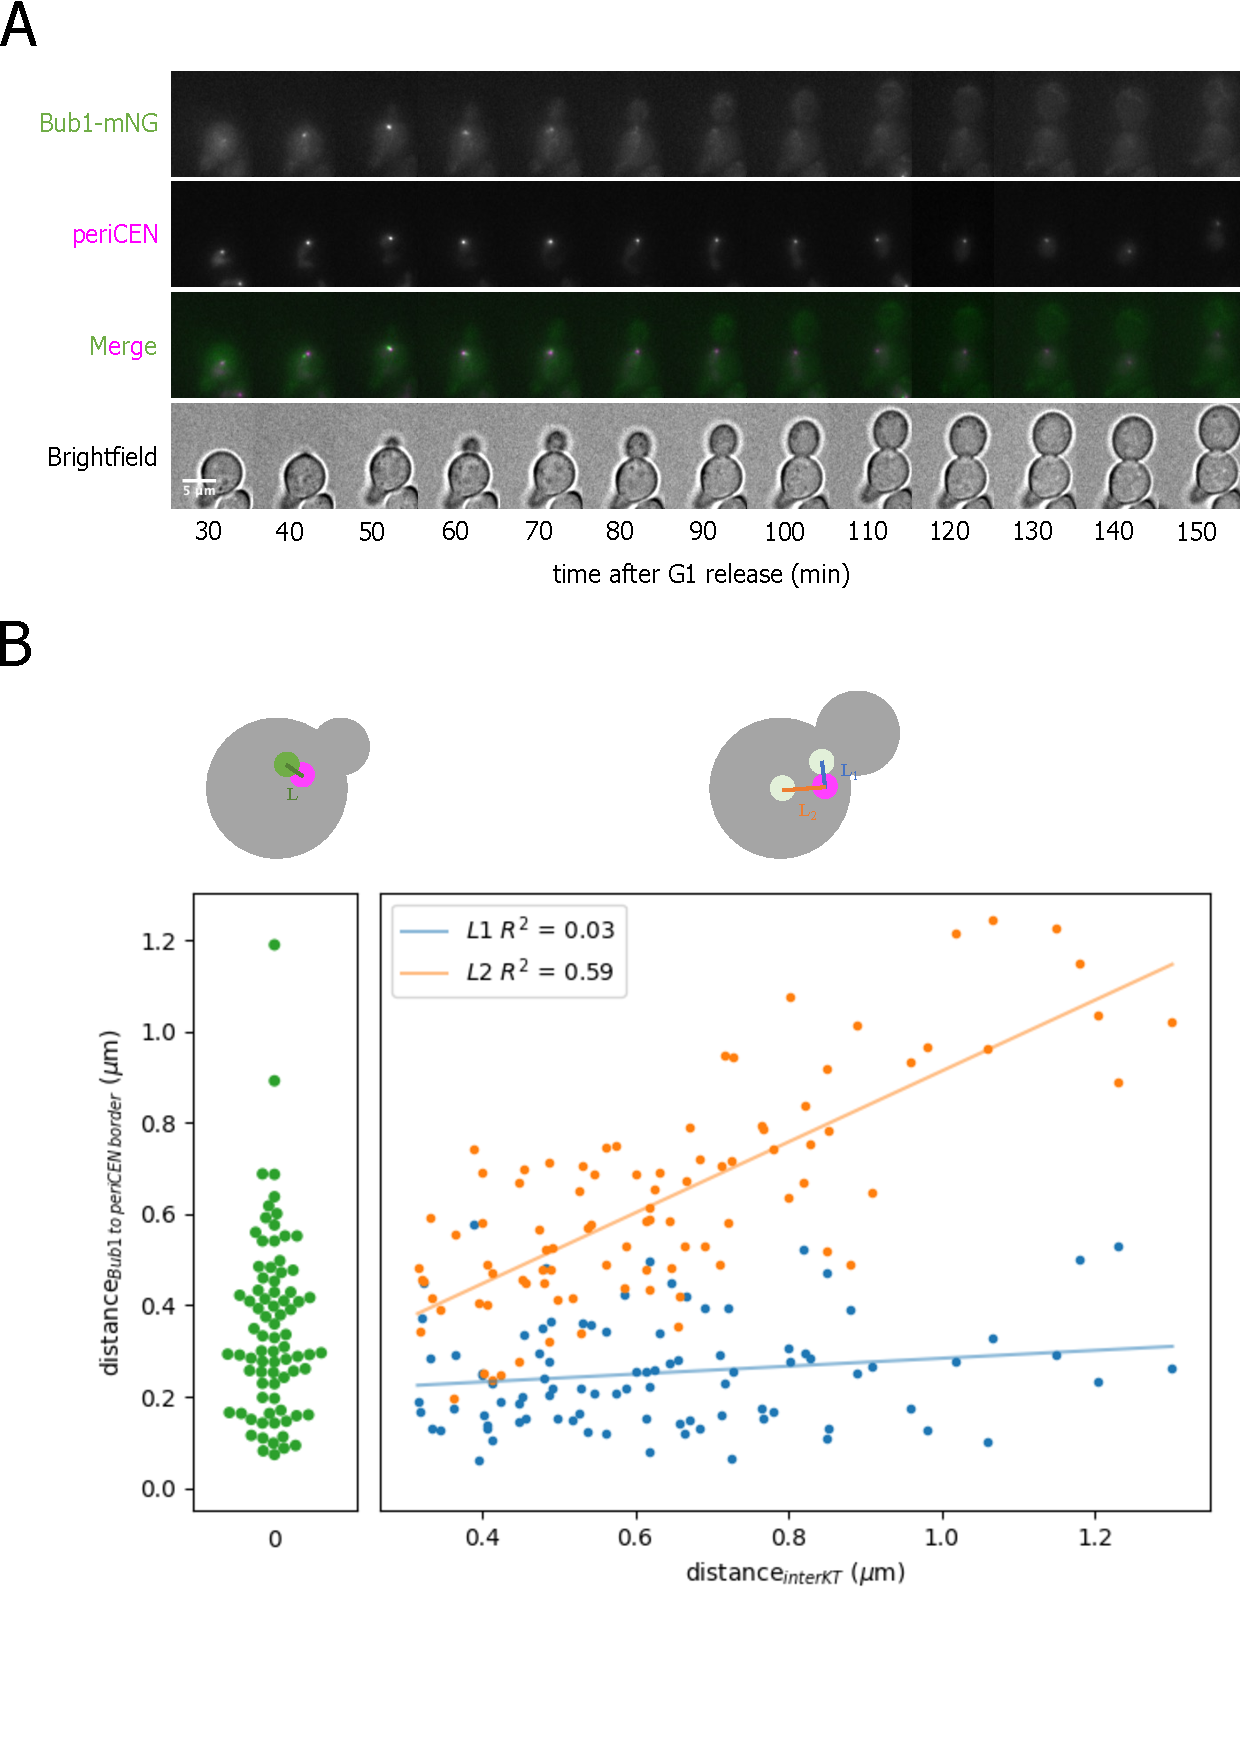
\includegraphics[width=0.9\textwidth]{figures/Bub1-mNG peri-cen.pdf}
  \caption[The shorter distance between Bub1 and peri-centromere is independent of the inter-kinetochore distance]{The shorter distance between Bub1 and peri-centromere is independent of the inter-kinetochore distance. (A) Montage of representative time-lapse imaging. (B) Scatter plot showing the relation of Bub1-to-peri-centromere distance and inter-kinetochore distance. N=30 cells were followed over time and quantified for $L$ (the distance before Bub1-mNG separation), $L_{1}$ (the shorter distance after Bub1-mNG separation) and $L_{2}$ (the longer distance after Bub1-mNG separation), which are presented in green, orange and blue, respectively. The line with the same colour represents the model of simple linear regression. }
  \label{fig:periCEN}
\end{figure} 

\nomenclature{mNG}{mNeonGreen}

\subsection{Bub1 is de-localised from the kinetochore by tension}
During data analysis of the previous experiment, I noticed a reduction in fluorescence intensity of Bub1-mNG foci as they separate to an extent that they are barely visible at the end of imaging. This cannot be simply explained by photo-bleaching because tdTomato is supposed to have a shorter bleaching time than mNG, yet it remains visible (Figure~\ref{fig:periCEN}A). The observation raises the possibility that the kinetochore localisation of Bub1 could be under the regulation of tension, leading to the physical separation from its substrates. The idea that Bub1 localisation could be regulated by tension has been implicated in literature \citep{Asai2020, Proudfoot2019, Jin2017PrematureCerevisiae}. To test this, I wanted to quantify the dynamics of the amount of Bub1 at the kinetochore as well as the inter-kinetochore distance. Since Bub1-mNG becomes indistinguishable from the background after separation, I chose to use the outer-kinetochore protein Mtw1 as a more reliable measure of the inter-kinetochore distance. I constructed a strain bearing \textit{BUB1-mNG MTW1-tdTomato pMET-CDC20}. Time-lapse live-cell imaging was again performed since the G1 release (Figure~\ref{fig:bub1mtw1}A). As expected, Bub1-mNG follows the same dynamics as in the previous experiment. While Mtw1-tdTomato appears as one focus at the start of imaging and then splits into two foci as the cell cycle progresses (Figure~\ref{fig:bub1mtw1}B). Further quantification showed that the fluorescence intensity of kinetochore Bub1-mNG peaks at 60 \si{\minute} since G1 release, with an over 2-fold decrease at 70 \si{\minute}, coinciding with the beginning of Mtw1-tdTomato foci separation (Figure~\ref{fig:bub1mtw1}C). This indicates that kinetochore-localised Bub1 is reduced upon the establishment of bi-orientation. 

\begin{figure}[htbp]
  \centering
  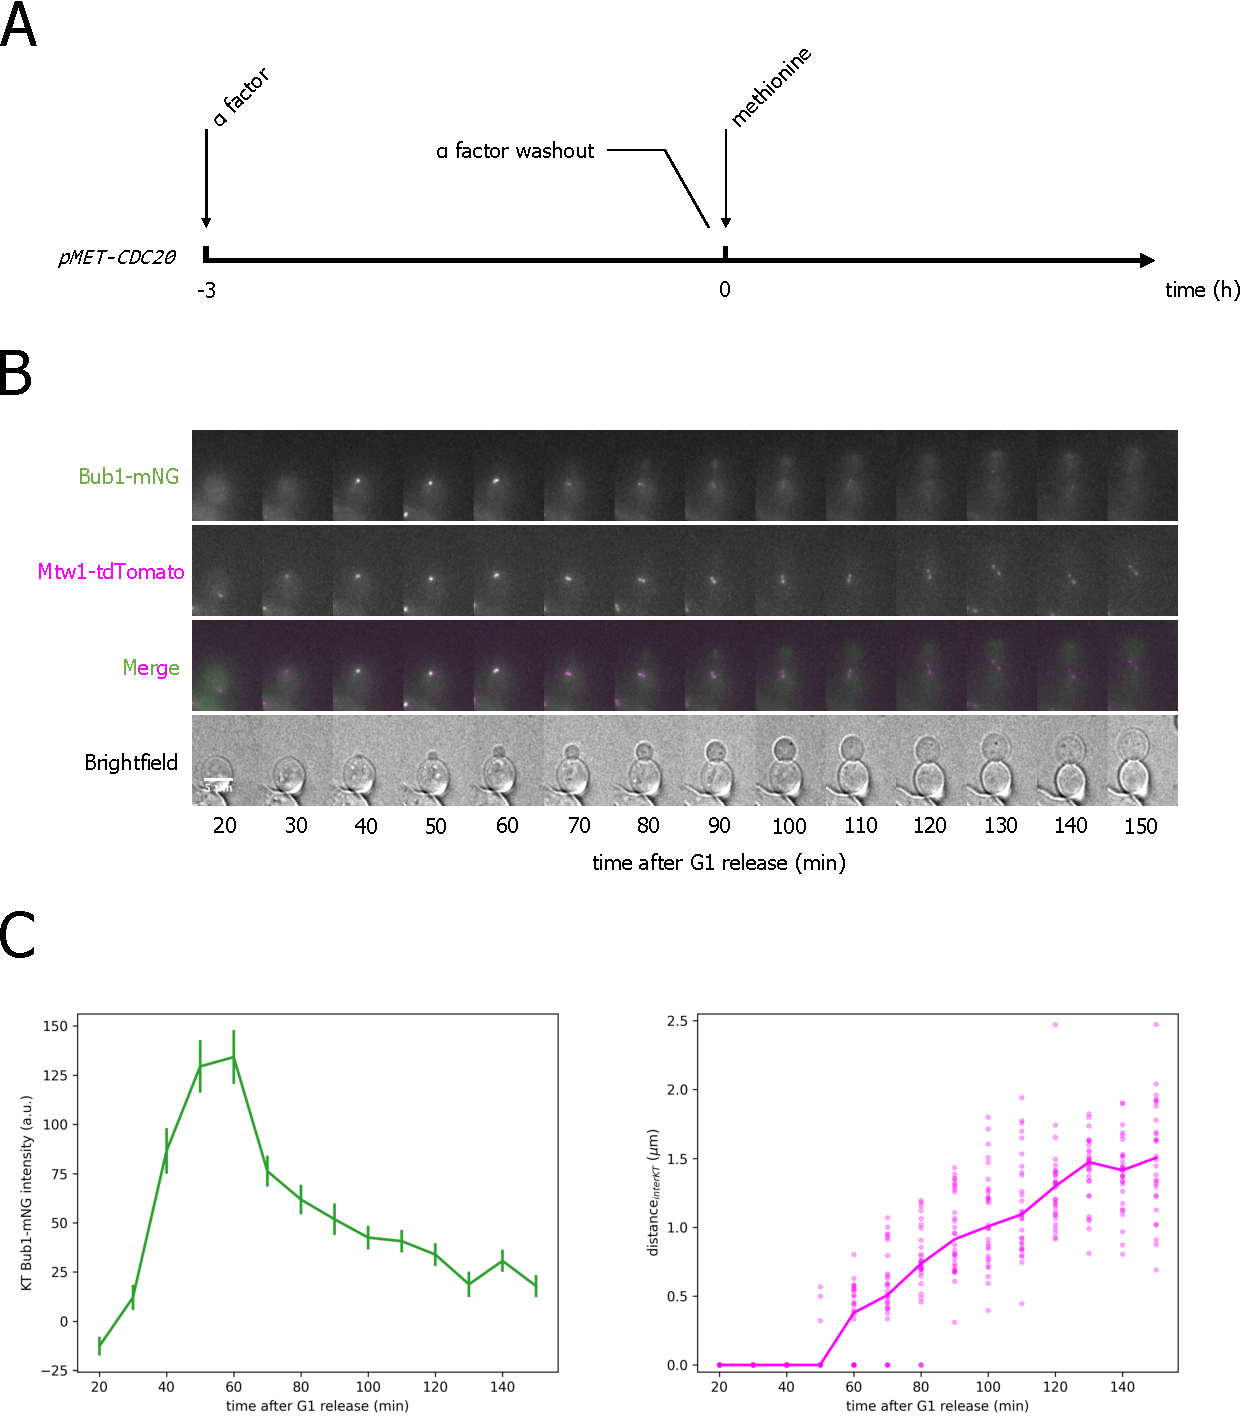
\includegraphics[width=0.9\textwidth]{figures/Bub1-mNG vs Mtw1-td.pdf}
  \caption[Kinetochore-localised Bub1 is reduced upon bi-orientation]{Kinetochore-localised Bub1 is reduced upon bi-orientation. (A) Schematics of experimental procedures. (B) Montage of representative time-lapse imaging. (C) N=30 cells were followed over time and quantified for kinetochore Bub1-mNG fluorescence intensity and inter-kinetochore distance. Left panel: mean fluorescence intensity of Bub1-mNG at the kinetochore as a function of time. The error bar represents the standard error. Right panel: Median inter-kinetochore distance as a function of time. Individual data points are shown as dots. }
  \label{fig:bub1mtw1}
\end{figure} 

I then sought to test whether the reduction in Bub1 kinetochore localisation is due to protein degradation or re-localisation. Human Bub1 is degraded by APC in anaphase \citep{Qi2007KEN-box-dependentComplex/cyclosome} but it is not known in budding yeast. Hence, I performed a synchronised mitotic time course experiment followed by western blotting to check Bub1 protein expression. Cells bearing \textit{BUB1-6HA} were synchronised in G1 and released into rich media. $\alpha$ factor was added 60 \si{\minute} after the release to arrest cells in the next G1 (Figure~\ref{fig:bub1timecourse}A). Tubulin IF was used to examine the progression of the cell cycle. At 75 \si{\minute} after G1 release, over 80\% of cells were in metaphase while most cells were in anaphase at 90 and 105 \si{\minute} (Figure~\ref{fig:bub1timecourse}B). Western blotting with anti-HA antibody showed Bub1 protein level reached its apex at 90 \si{\minute} and started to decrease since 105 \si{\minute} (Figure~\ref{fig:bub1timecourse}C), suggesting Bub1 is degraded in late anaphase in budding yeast. Therefore, protein degradation could not be the reason for reduced Bub1 kinetochore localisation in metaphase in the previous experiment. Interestingly, Bub1 experienced changes in electrophoretic mobility at the early stage of the cell cycle, indicating its phosphorylation status might be actively regulated. As this is beyond the scope of my project, this was not investigated further. 

\begin{figure}[htbp]
  \centering
  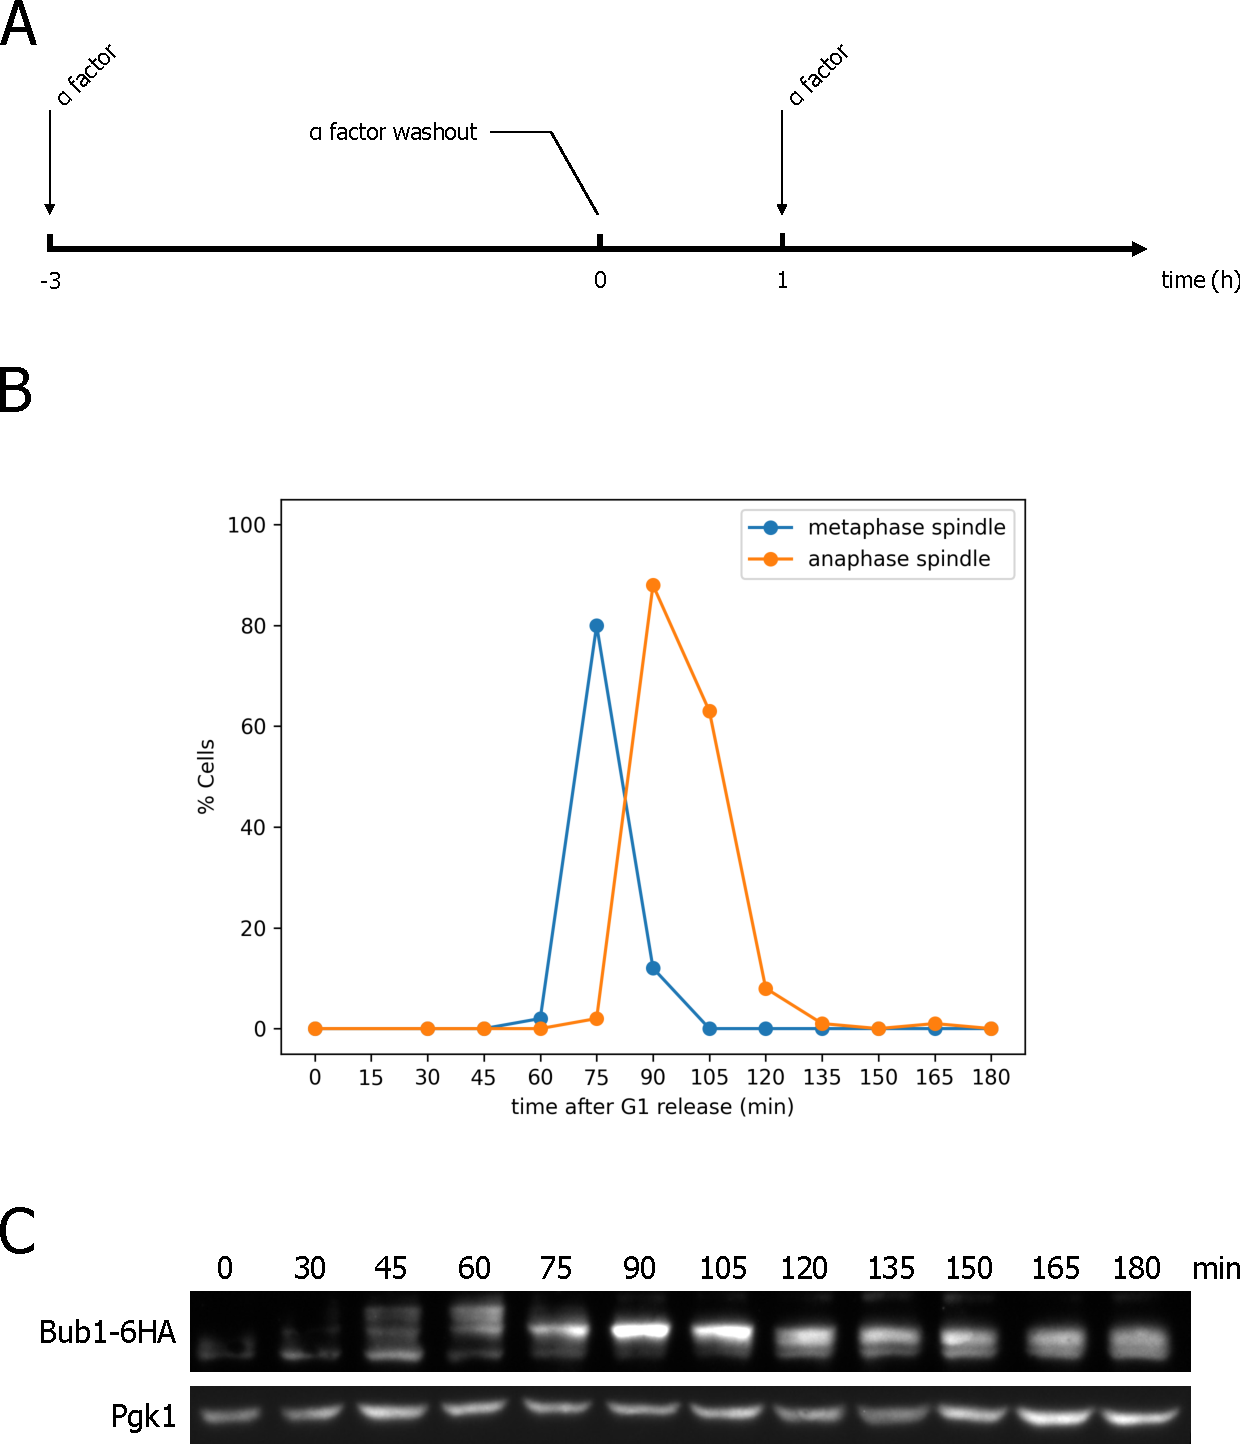
\includegraphics[width=0.9\textwidth]{chapter3/figures/Bub1-6HA time course.pdf}
  \caption[Bub1 is not degraded until anaphase]{Bub1 is not degraded until anaphase. (A) Schematics of experimental procedures. (B) The proportion of cells with metaphase or anaphase spindle over time by tubulin IF. (C) Western blotting with anti-HA antibody to detect Bub1 protein. Pgk1 was used as the loading control.}
  \label{fig:bub1timecourse}
\end{figure} 

The experiments above suggest that Bub1 is re-localised from the kinetochore upon bi-orientation. Given that both tension and kinetochore-microtubule attachment are established in this case, it is unkown whether tension is required for Bub1 de-localisation besides attachment. To abolish tension without disrupting attachment, I decided to disable sister chromatid cohesion by depleting the kleisin subunit Scc1 of the cohesin complex. Cells from Figure~\ref{fig:bub1mtw1} with or without additional \textit{pMET-SCC1} were synchronised in G1. Methionine was added 45 \si{\minute} before releasing to pre-clean Scc1 in the \textit{pMET-SCC1} strain. Live-cell imaging was performed to quantify kinetochore Bub1-mNG fluorescence intensity and inter-kinetochore distance (Figure~\ref{fig:bub1metscc1}A). As expected, the \textit{pMET-SCC1} strain exhibited increased inter-kinetochore distance ($\sim$2.5 \si{\micro\metre} towards the end of the experiment) compared to the wild type ($\sim$1.5 \si{\micro\metre} towards the end of the experiment), indicating a reduction in sister chromatid cohesion. Unlike the wild type, the signal of kinetochore Bub1-mNG is maintained at a similar value after 60 \si{\minute} from G1 release in the \textit{pMET-SCC1} strain (Figure~\ref{fig:bub1metscc1}B and C), suggesting Bub1 is not removed from the kinetochore in the absence of tension while no additional disruption was applied on attachment. To rule out the potential artefacts from \textit{pMET-SCC1} causing an increase in Bub1 expression, I used western blotting to check the Bub1 protein expression level in the wild type and the \textit{pMET-SCC1} strain arrested in metaphase by methionine depletion. No obvious difference was observed (Figure~\ref{fig:bub1metscc1}D). Hence, the kinetochore localisation of Bub1 is reduced by tension. 

\begin{figure}[htbp]
  \centering
  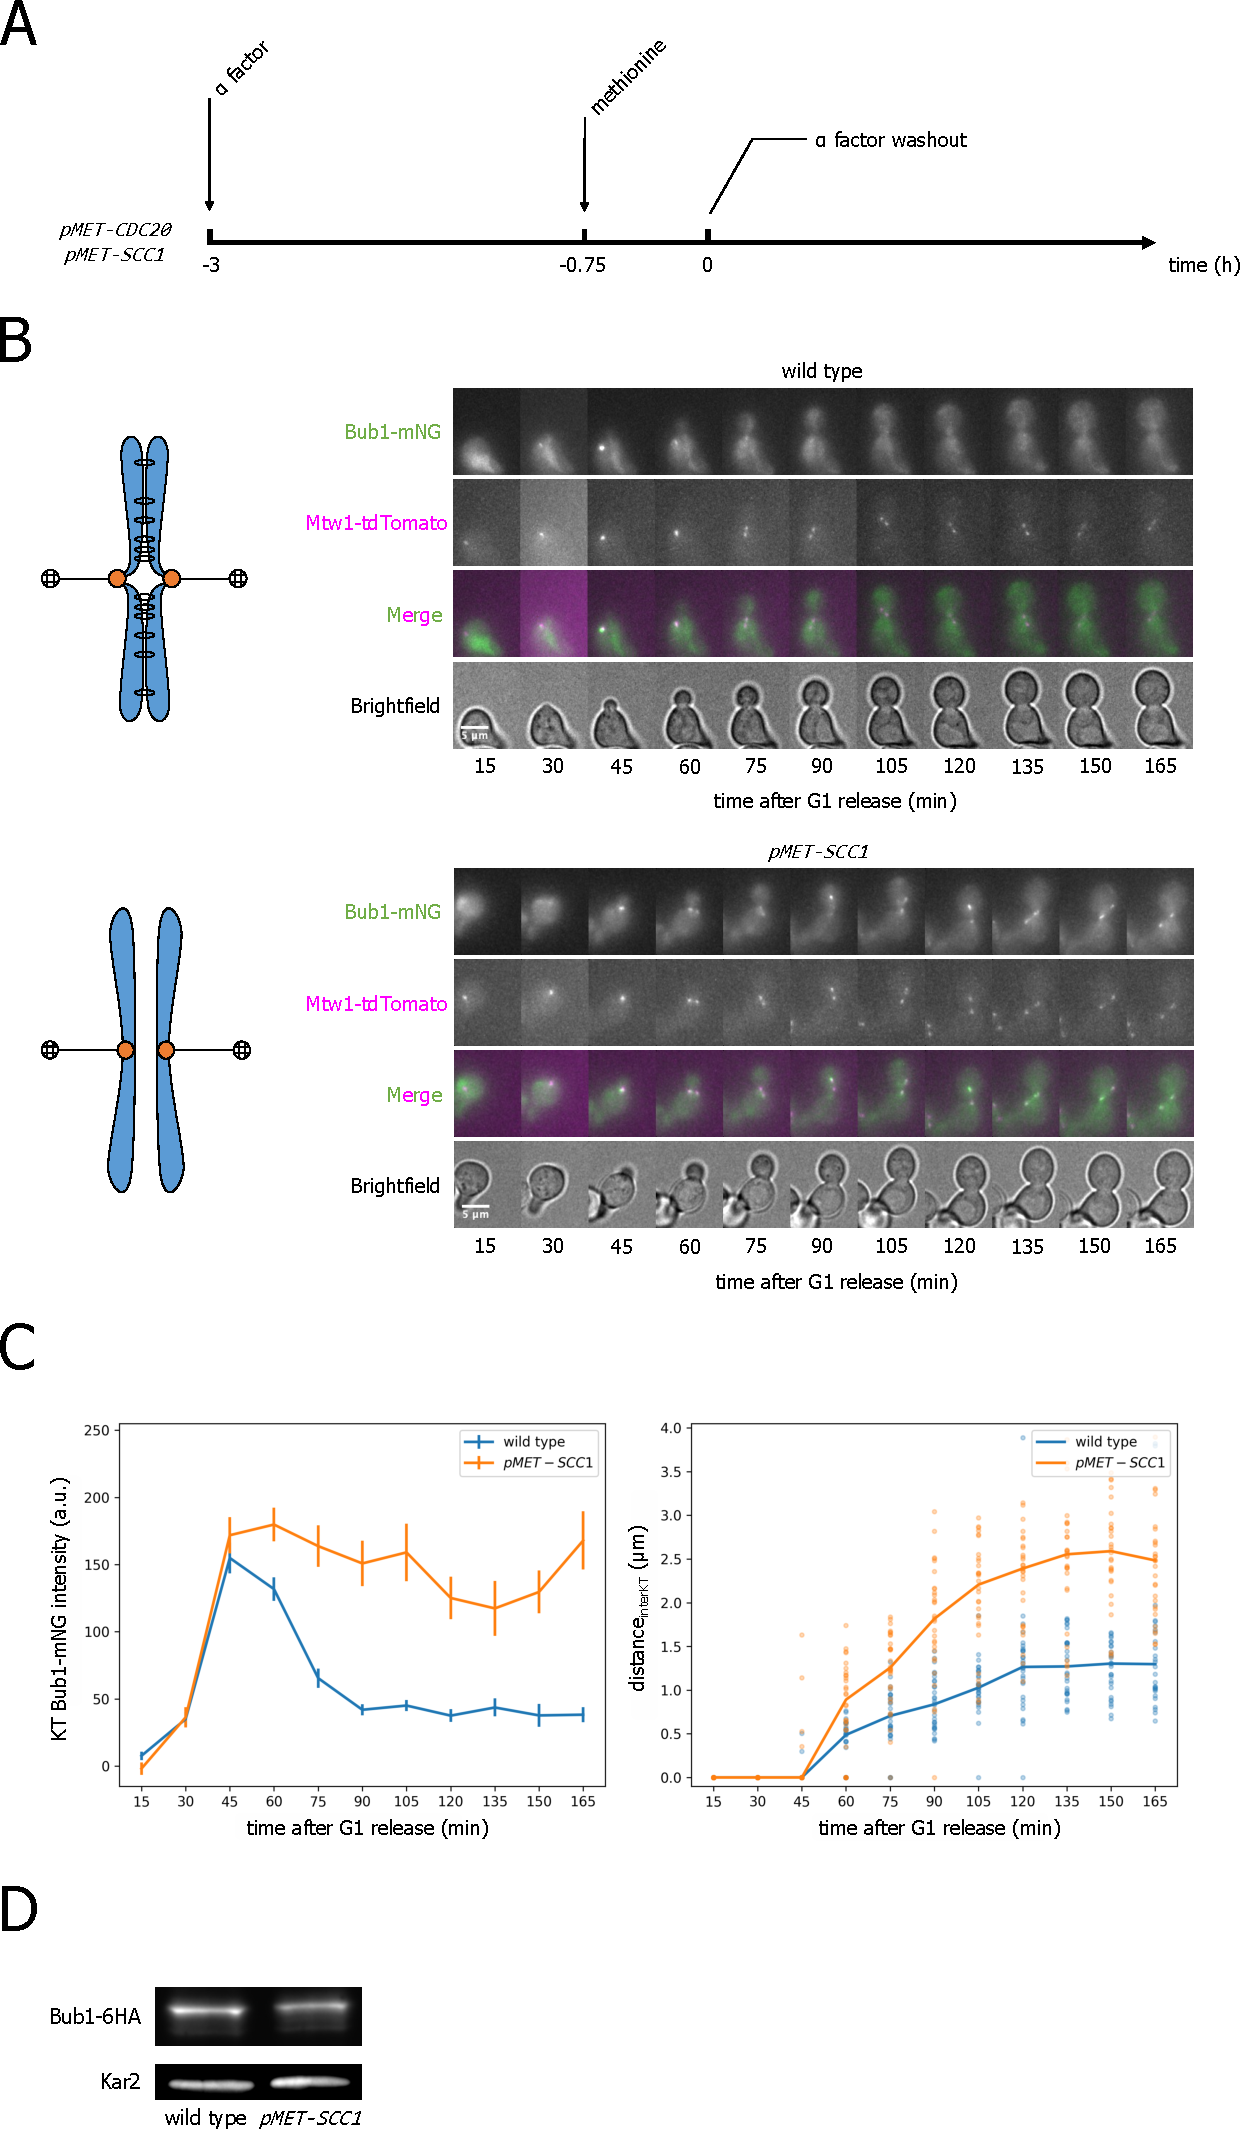
\includegraphics[width=0.9\textwidth]{chapter3/figures/Bub1-mNG pMET-SCC1.pdf}
  \caption[Tension is required for Bub1 re-localisation from the kinetochore]{Tension is required for Bub1 re-localisation from the kinetochore. (A) Schematics of experimental procedures. (B) Montage of representative time-lapse imaging. Cartoons on the left indicate the status of sister chromatids. (C) N=30 cells for each strain were followed over time and quantified for kinetochore Bub1-mNG fluorescence intensity and inter-kinetochore distance. Left panel: mean fluorescence intensity of Bub1-mNG at the kinetochore as a function of time. The error bar represents the standard error. Right panel: Median inter-kinetochore distance as a function of time. Individual data points are shown as dots. The wild type is shown in blue and \textit{pMET-SCC1} is shown in orange. (D) Western blotting with anti-HA antibody to detect Bub1 protein. Kar2 was used as the loading control. }
  \label{fig:bub1metscc1}
\end{figure} 

\subsection{Bub1 removal is sufficient for rapid de-localisation of Sgo1}
\cite{Nerusheva2014} have shown with ChIP-qPCR that Bub1 depletion abolishes Sgo1 localisation at the peri-centromere in the absence of tension, suggesting Bub1 removal triggers Sgo1 de-localisation. However, the 1 \si{\hour} time resolution of the experiment was not fine enough to explain the fast kinetics of Sgo1 re-localisation, where the transition from focused to diffused signal happens within 15 \si{\minute}. To repeat this result with an independent method as well as to improve the time resolution, I sought to repeat this experiment with microscopy. \textit{SGO1-EGFP MTW1-tdTomato pMET-CDC20} strain with additional AID system to deplete Bub1 (\textit{BUB1-3V5-AID} P$_{ADH1}$\textit{-OsTIR1-9MYC}) was synchronised in G1 and then released into nocodazole-containing media for a metaphase arrest without tension. Since Bub1 is a component of SAC, the media also does not contain methionine to prevent anaphase onset when Bub1 is depleted. Auxin NAA was then added to induce Bub1 depletion, with imaging started immediately (Figure~\ref{fig:bub1aid}A). Consistent with previous research, nocodazole-arrested cells showed large buds and signals of 2 or 3 dots for both Sgo1-EGFP and Mtw1-tdTomato \citep{Richmond2013Slk19Attachment}. In contrast to the control where DMSO was added (-NAA), Sgo1-EGFP foci disappeared after the addition of NAA (+NAA) (Figure~\ref{fig:bub1aid}C). Survival analysis indicated that the probability for cells to have a Sgo1-EGFP dot-signal started to decrease since NAA was added, with less than 20\% at 30 \si{\minute} afterwards (Figure~\ref{fig:bub1aid}D). To verify the depletion of Bub1 as well as characterising its kinetics, I performed western blotting on time course samples of cells treated identically as in the imaging experiment. The level of Bub1 protein became largely reduced at 20 \si{\minute} and barely detectable from 30 \si{\minute} after adding NAA (Figure~\ref{fig:bub1aid}E), similar to the dynamics of Sgo1 de-localisation shown in Figure~\ref{fig:bub1aid}D. This suggests a very quick response of Sgo1 localisation to Bub1 depletion, which could explain the fast re-localisation of Sgo1 previously observed \citep{Nerusheva2014}. Therefore, it is possible that the tension-dependent re-localisation of Sgo1 results from the de-localisation of Bub1 from the kinetochore by tension. 

\nomenclature{AID}{Auxin-Inducible Degron}
\nomenclature{NAA}{Naphthalene Acetic Acid}
\nomenclature{DMSO}{DiMethyl SulfOxide}

\begin{figure}[htbp]
  \centering
  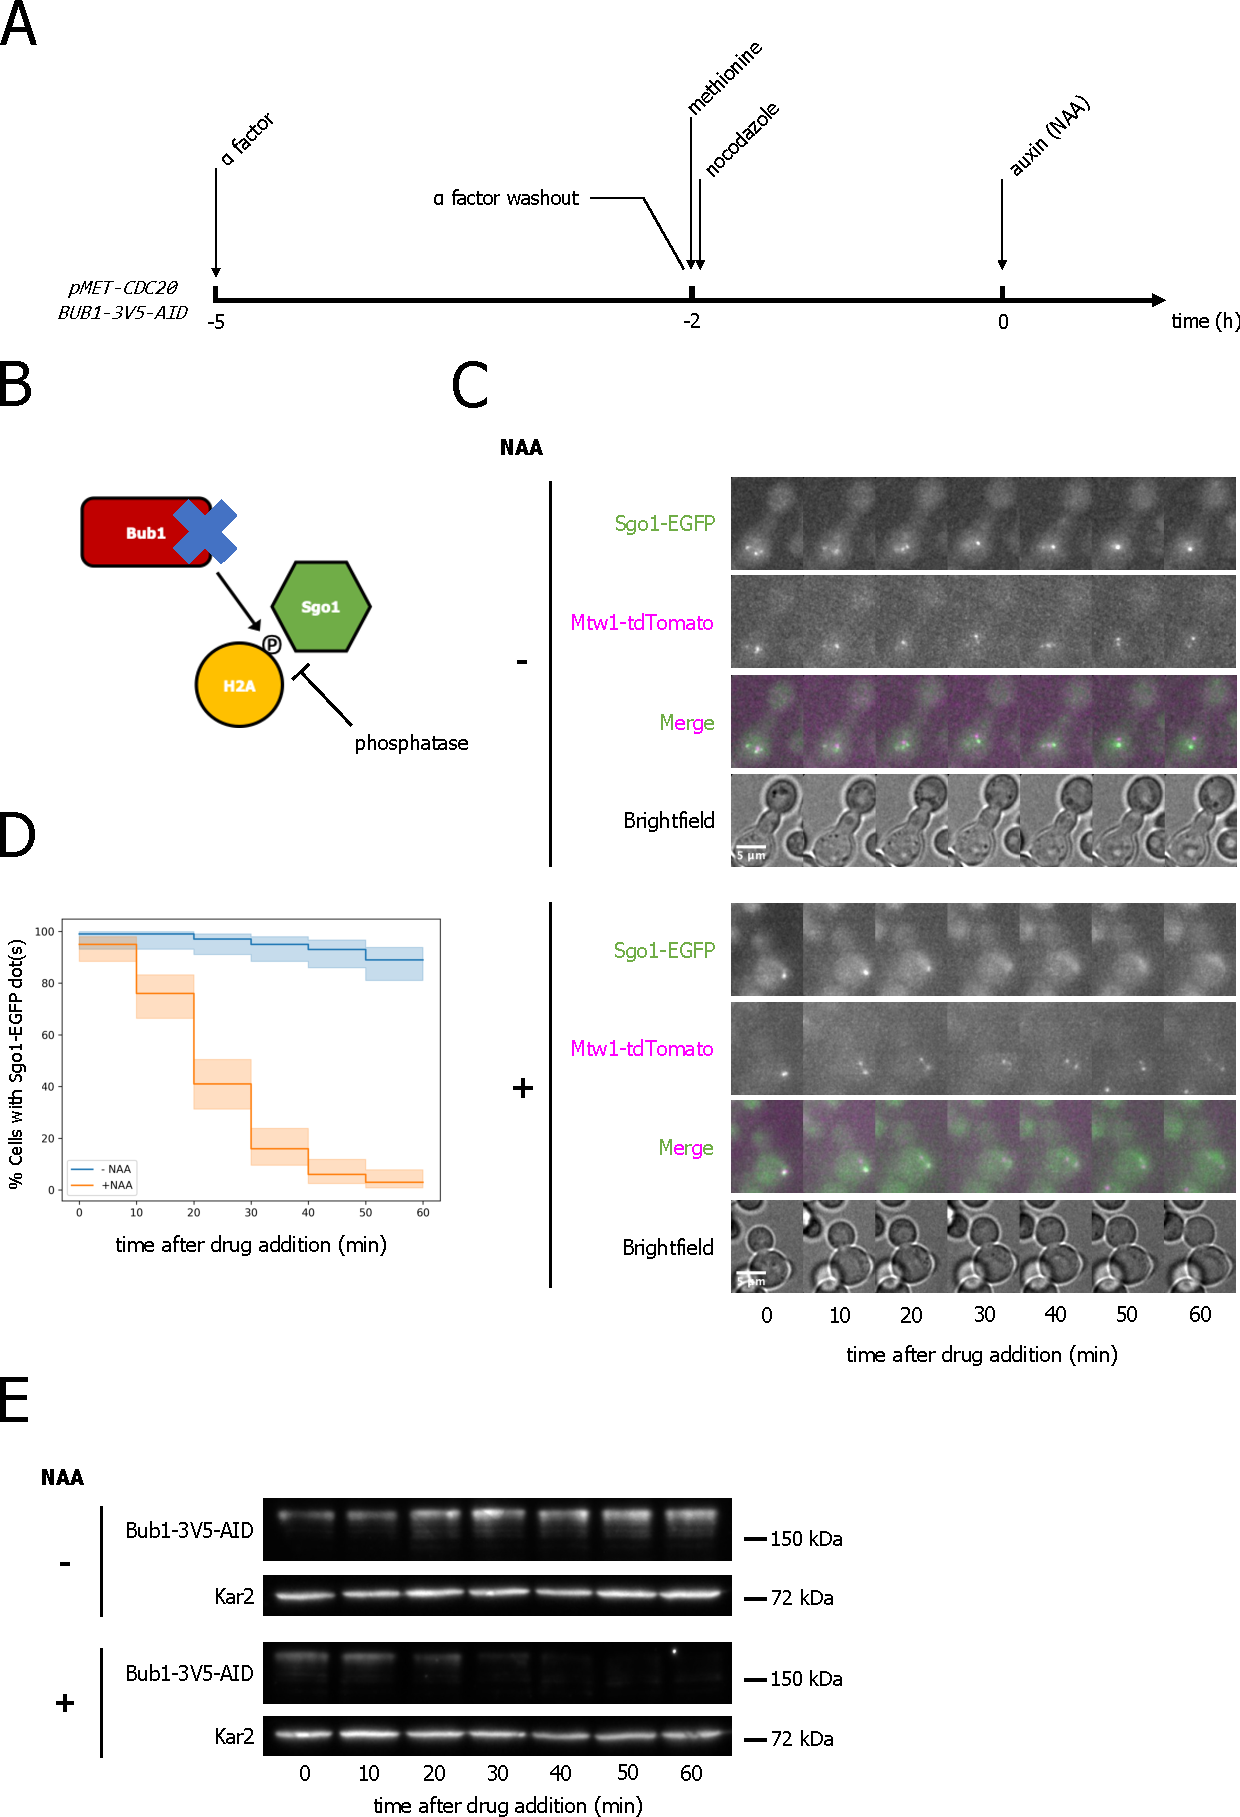
\includegraphics[width=0.9\textwidth]{chapter3/figures/Bub1-3V5-AID.pdf}
  \caption[Sgo1 is de-localised promptly upon Bub1 depletion in the absence of tension]{Sgo1 is de-localised promptly upon Bub1 depletion in the absence of tension. (A) Schematics of experimental procedures. (B) Schematics of experimental concept. (C) Montage of representative time-lapse imaging. (D) Survival analysis of the duration of focused Sgo1-EGFP signal. N=100 cells for each strain were followed over time and quantified for the duration of the Sgo1-EGFP signal being focused. Solid lines are Kaplan-Meier survival estimates. The shaded area in the same colour is the 95\% confidence limit of the estimate. (E) Western blotting with anti-V5 antibody to detect Bub1 protein. Kar2 was used as the loading control.}
  \label{fig:bub1aid}
\end{figure} 

\subsection{Bub1 re-localisation is earlier than Sgo1 re-localisation}
The data so far have suggested a model where Bub1 and Sgo1 re-localise sequentially. If this is true, there could be a difference in the timing of their re-localisation. To test it, a strain with the two proteins tagged with fluorescence proteins of different colours should be used in the ideal situation. However, none of Bub1 or Sgo1 tagged with various RFPs gave good enough signals under our microscope, possibly due to a combination of low abundance and cell-cycle-dependent expression of the two proteins. For example, Sgo1 tagged with the brightest RFP in the lab tdTomato is visible as dots in cells arrested with nocodazole but not in an unperturbed cell cycle because tdTomato has a maturation time beyond the time Sgo1 can be detected in a mitotic time course \citep{Indjeian2005a}. Instead, I could only image Bub1-mNG and Sgo1-EGFP in separate strains and use the inter-kinetochore distance measured from Mtw1-tdTomato as the internal control for timing. Standard G1 to metaphase live-cell imaging was carried out (Figure~\ref{fig:bub1sgo1}A). The inter-kinetochore distances are indistinguishable between the two strains (Figure~\ref{fig:bub1sgo1}B), suggesting a similar progress of tension establishment. Kinetochore Bub1-mNG fluorescence intensity was quantified as in the previous experiments. Due to the fact that Sgo1-EGFP is close to but does not co-localise with the kinetochore, it was not able to define the ROI to quantify fluorescence intensity. Therefore, Sgo1-EGFP was only scored for whether the signal can be counted as focused or not. Consistent with the speculation, the dynamics of Sgo1-EGFP and Bub1-mNG were similar except for a 15 \si{\minute} delay of Sgo1-EGFP in both the increase and decrease (Figure~\ref{fig:bub1sgo1}B), supporting the idea that Bub1 removal from the kinetochore triggers the de-localisation of Sgo1. 

\nomenclature{ROI}{Region Of Interest}

\begin{figure}[htbp]
  \centering
  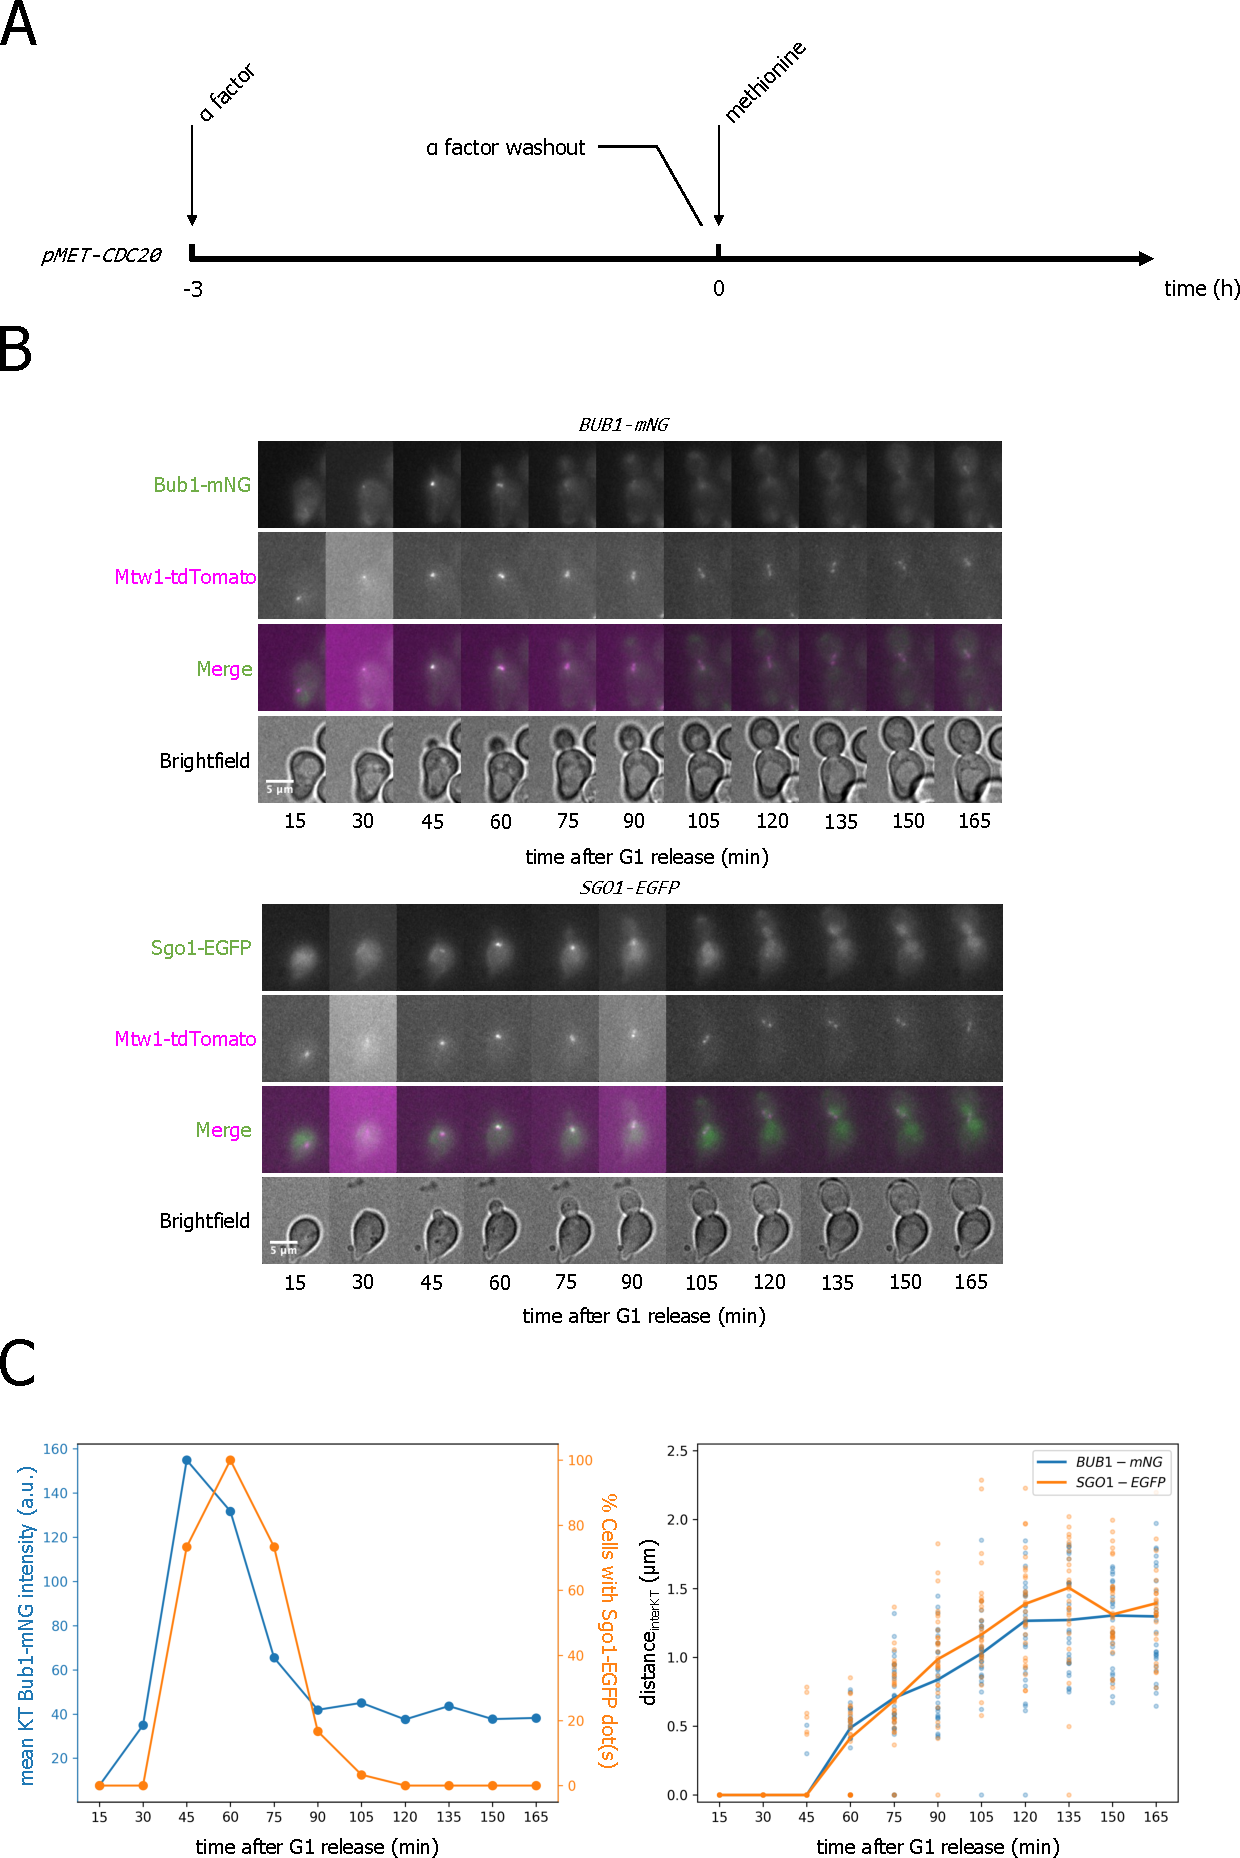
\includegraphics[width=0.9\textwidth]{chapter3/figures/Bub1-mNG Sgo1-EGFP.pdf}
  \caption[Bub1 is re-localised earlier than Sgo1]{Bub1 is re-localised earlier than Sgo1. (A) Montage of representative time-lapse imaging. (B) N=30 cells for each strain were followed over time and quantified. Left panel: mean fluorescence intensity of Bub1-mNG at the kinetochore and percentage of cells with Sgo1 foci as a function of time. Right panel: Median inter-kinetochore distance as a function of time. Individual data points are shown as dots. The \textit{BUB1-mNG} strain is shown in blue and the \textit{SGO1-EGFP} strain is shown in orange.}
  \label{fig:bub1sgo1}
\end{figure} 

\subsection{The continued presence of Bub1 is required to maintain H2A-pS121}
Our naive model argues that the phosphorylation status of the key substrate(s) determining Sgo1 localisation should be regulated by the kinase-phosphatase balance between Bub1 and unknown phosphatase(s) (Figure~\ref{fig:naive}). Therefore, the substrate(s) is expected to be phosphorylated in the absence of tension and de-phosphorylated when existing Bub1 is depleted as in the previous experiment (Figure~\ref{fig:ph2abub1aid}B). Given the demonstrated role of H2A-pS121 in localising Sgo1 to the peri-centromere \citep{Kawashima2010a, Fernius2007Bub1Mitosis, Nerusheva2014}, I hypothesised that it is the key Bub1 substrate being regulated. To directly monitor the phosphorylation status of H2A-S121, I ordered phospho-specific antibodies from Genscript. Western blotting using these antibodies indicated that they are able to distinguish phosphorylated H2A-S121 from unphosphorylated one as there is a less-than-17-\si{\kilo\dalton} band bright in wild type but extremely dim in Bub1 kinase-dead mutant (\textit{bub1$\Delta$K}) or H2A phospho-null mutant (H2A-S121A) arrested by nocodazole (Figure~\ref{fig:abtest}). 

\begin{figure}[htbp]
  \centering
  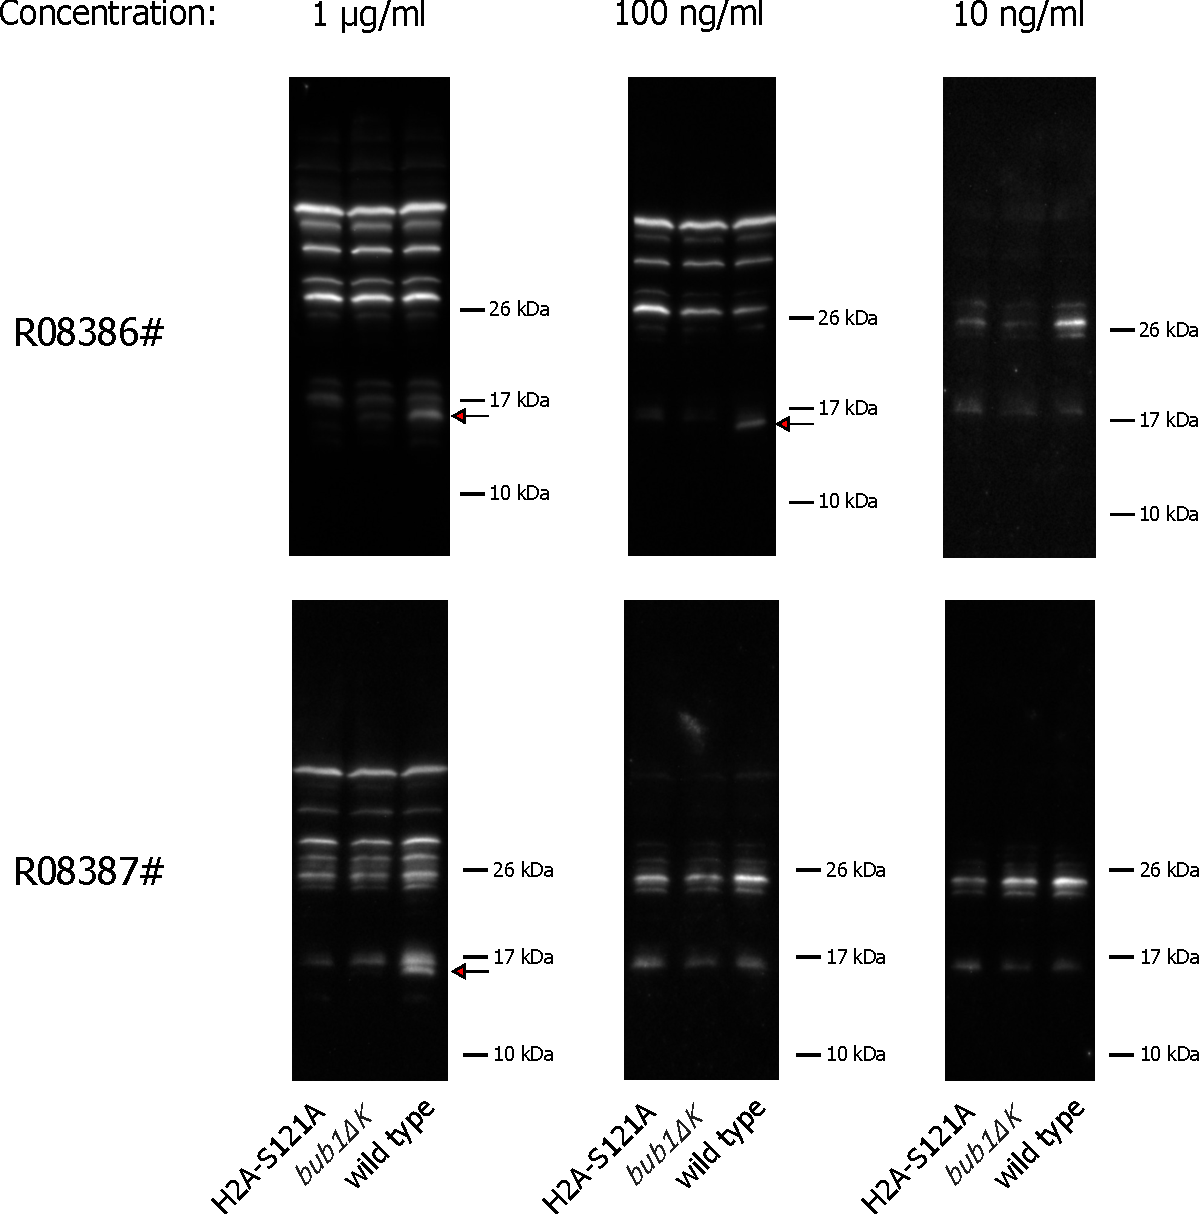
\includegraphics[width=0.9\textwidth]{chapter3/figures/pH2A ab test.pdf}
  \caption[Validation of phospho-specific antibodies for H2A-pS121]{Validation of phospho-specific antibodies for H2A-pS121. Western blotting on H2A-S121A, \textit{bub1$\Delta$K} or wild type arrested by nocodazole using anti-Hta2-pS122 antibodies generated from host R08386\# or R08387\# (GenScript) at 1 \si{\micro\gram/\milli\litre}, 100 \si{\nano\gram/\milli\litre} or 10 \si{\nano\gram/\micro\litre}. Red arrows indicate the specific bands. }
  \label{fig:abtest}
\end{figure} 

To test whether H2A is indeed de-phosphorylated at S121 upon Bub1 depletion, I conducted western blotting on samples from the experiment of Figure~\ref{fig:bub1aid} (Figure~\ref{fig:ph2abub1aid}A). The specific band is maintained within the scope of the experiment in -NAA samples. In contrast, it is reduced in +NAA samples in spite of the increase in the intensity of the non-specific band above (Figure~\ref{fig:ph2abub1aid}C), suggesting that H2A-pS121 is being de-phosphorylated due to Bub1 depletion. Hence, the continued presence of Bub1 is required to maintain H2A-pS121, favouring the naive model and the idea that H2A-pS121 is the key substrate. Due to the non-ideal specificity of the antibody over unphosphorylated H2A-S121, it is difficult to interpret the kinetics of the de-phosphorylation. 

\begin{figure}[htbp]
  \centering
  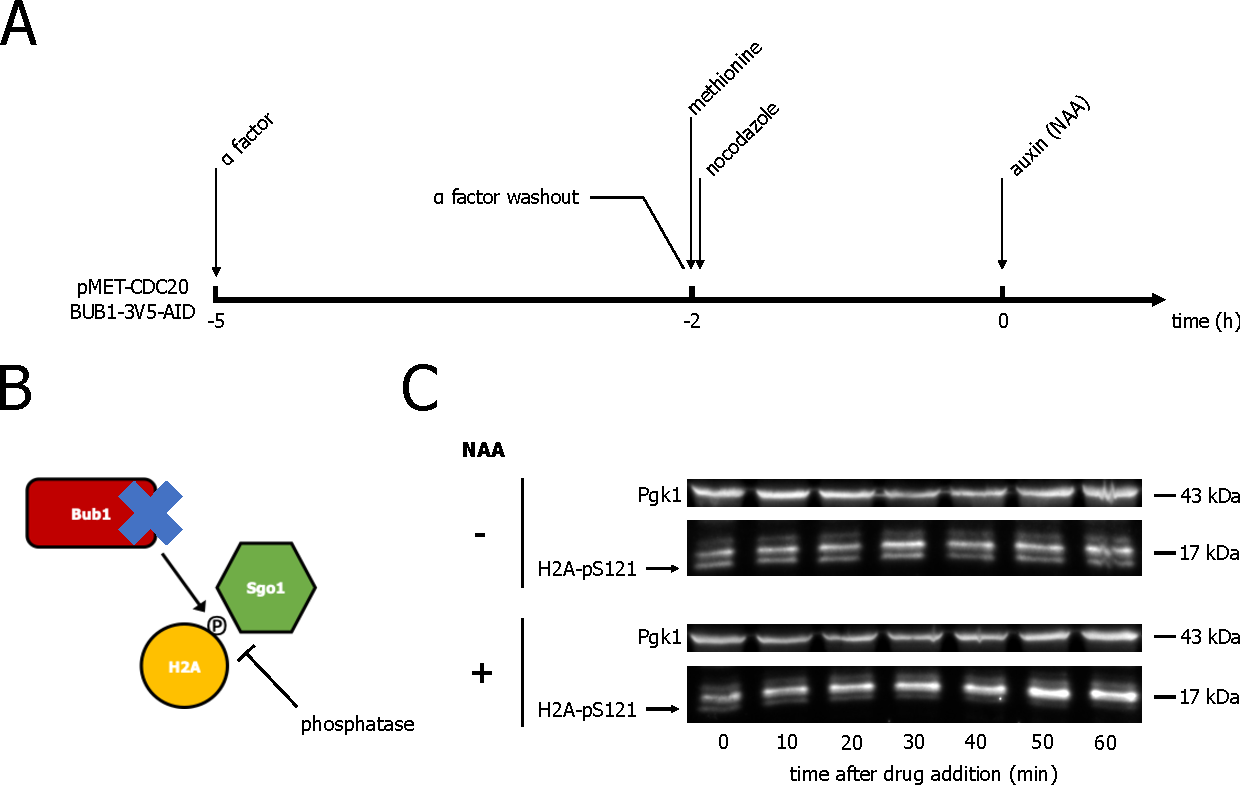
\includegraphics[width=0.9\textwidth]{chapter3/figures/pH2A Bub1-AID.pdf}
  \caption[Bub1 depletion leads to a reduction in H2A-S121 phosphorylation in the absence of tension]{Bub1 depletion leads to a reduction in H2A-S121 phosphorylation in the absence of tension. (A) Schematics of experimental procedures. (B) Schematics of experimental concept. (C) Western blotting with anti-H2A-pS121 antibody to detect the phosphorylation status of H2A. Pgk1 was used as the loading control.}
  \label{fig:ph2abub1aid}
\end{figure} 

\subsection{Total cellular H2A-pS121 level is independent of tension}
\label{subsec:totalph2aindten}

Since tension de-localises Bub1 from the kinetochore, physically separating it from its substrate H2A at the peri-centromere, I hypothesised that the phosphorylation of H2A-S121 would be lost or at least reduced by tension. Therefore, I arrested wild type strain, the control strain used for imaging and the negative control \textit{bub1$\Delta$K} in the presence or absence of tension (Figure~\ref{fig:ph2atension}A). Western blotting against H2A-pS121 was conducted as before. Surprisingly, tension did not decrease the intensity of the specific band for both wild type and the imaging strain (Figure~\ref{fig:ph2atension}B), indicating the level of total cellular H2A-pS121 is independent of tension. It seems that tension even increased the specific band intensity for the imaging strain. However, I believe it is due to the variation in the blotting process, as the intensity of the non-specific band is also reduced in the no tension sample compared to the tension sample. 

\begin{figure}[htbp]
  \centering
  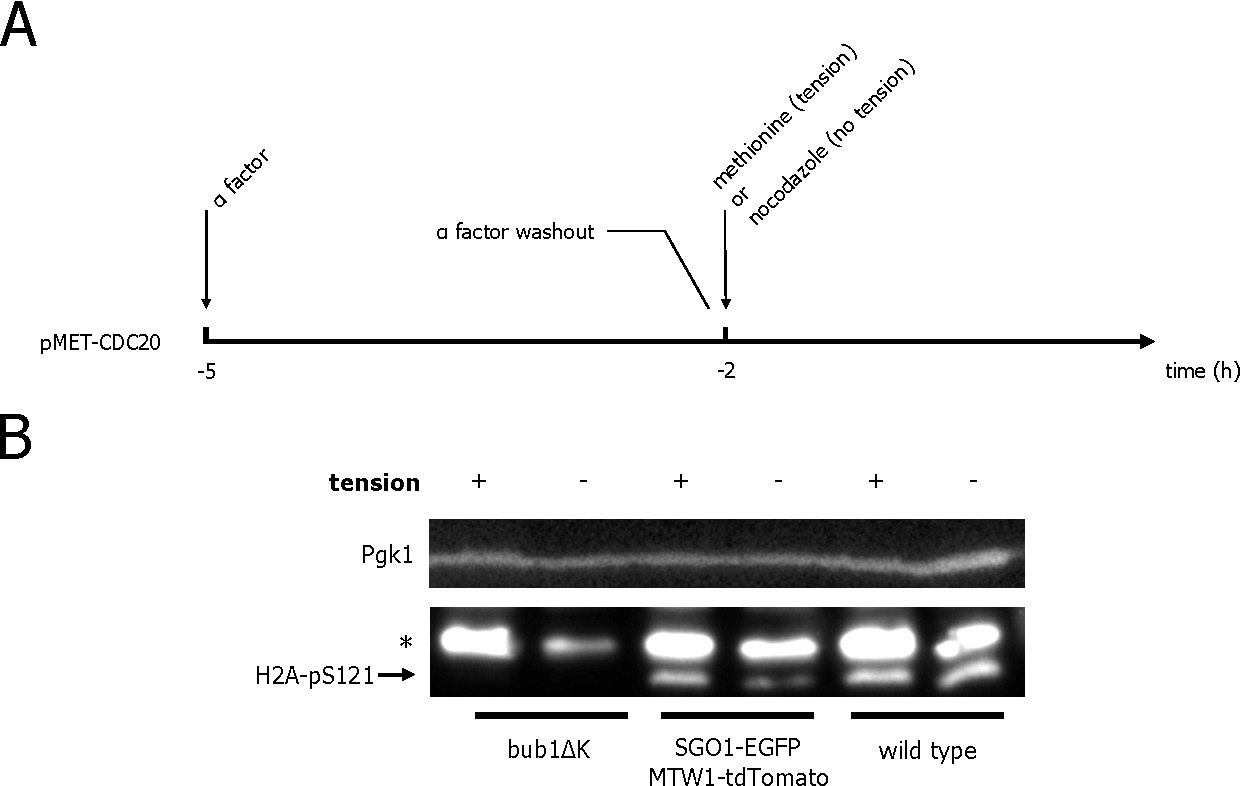
\includegraphics[width=0.9\textwidth]{chapter3/figures/pH2A tension.pdf}
  \caption[Total cellular H2A-pS121 level is independent of tension]{Total cellular H2A-pS121 level is independent of tension.(A) Schematics of experimental procedures. (B) Western blotting with anti-H2A-pS121 antibody to detect the phosphorylation status of H2A. Pgk1 was used as the loading control. The asterisk represents the non-specific band.}
  \label{fig:ph2atension}
\end{figure}

To validate this unexpected result, I turned to a different approach where H2A-pS121 were monitored over the entire cell cycle. Cells bearing \textit{PDS1-HA} were synchronised in G1 and released into rich media as described in the previous synchronised mitotic time course experiment (Figure~\ref{fig:ph2atimecourse}A). Tubulin IF indicated that most cells were in metaphase at 75 \si{\minute} after G1 release while in anaphase at 90 and 105 \si{\minute} (Figure~\ref{fig:ph2atimecourse}B). Western blotting with anti-HA and anti-H2A-pS121 was then performed on the time course samples. The securin Pds1 peaked at 75 \si{\minute} and became barely visible at 90 \si{\minute}, consistent with the cell cycle stages information from the tubulin IF. The H2A-pS121 band was comparable from 60 to 90 \si{\minute}, with a sharp reduction at 105 \si{\minute}, suggesting the level of H2A-pS121 is maintained during the metaphase-anaphase transition, therefore verifying the previous result. The reason that the non-specific bands here appeared differently from the previous experiments is likely due to the fact that I used a large protein gel in this western blotting for better protein resolution. Interestingly, the dynamics of H2A-pS121 level over the cell cycle are qualitatively similar to that of Bub1 protein level (Figure~\ref{fig:bub1timecourse}). 

\begin{figure}[htbp]
  \centering
  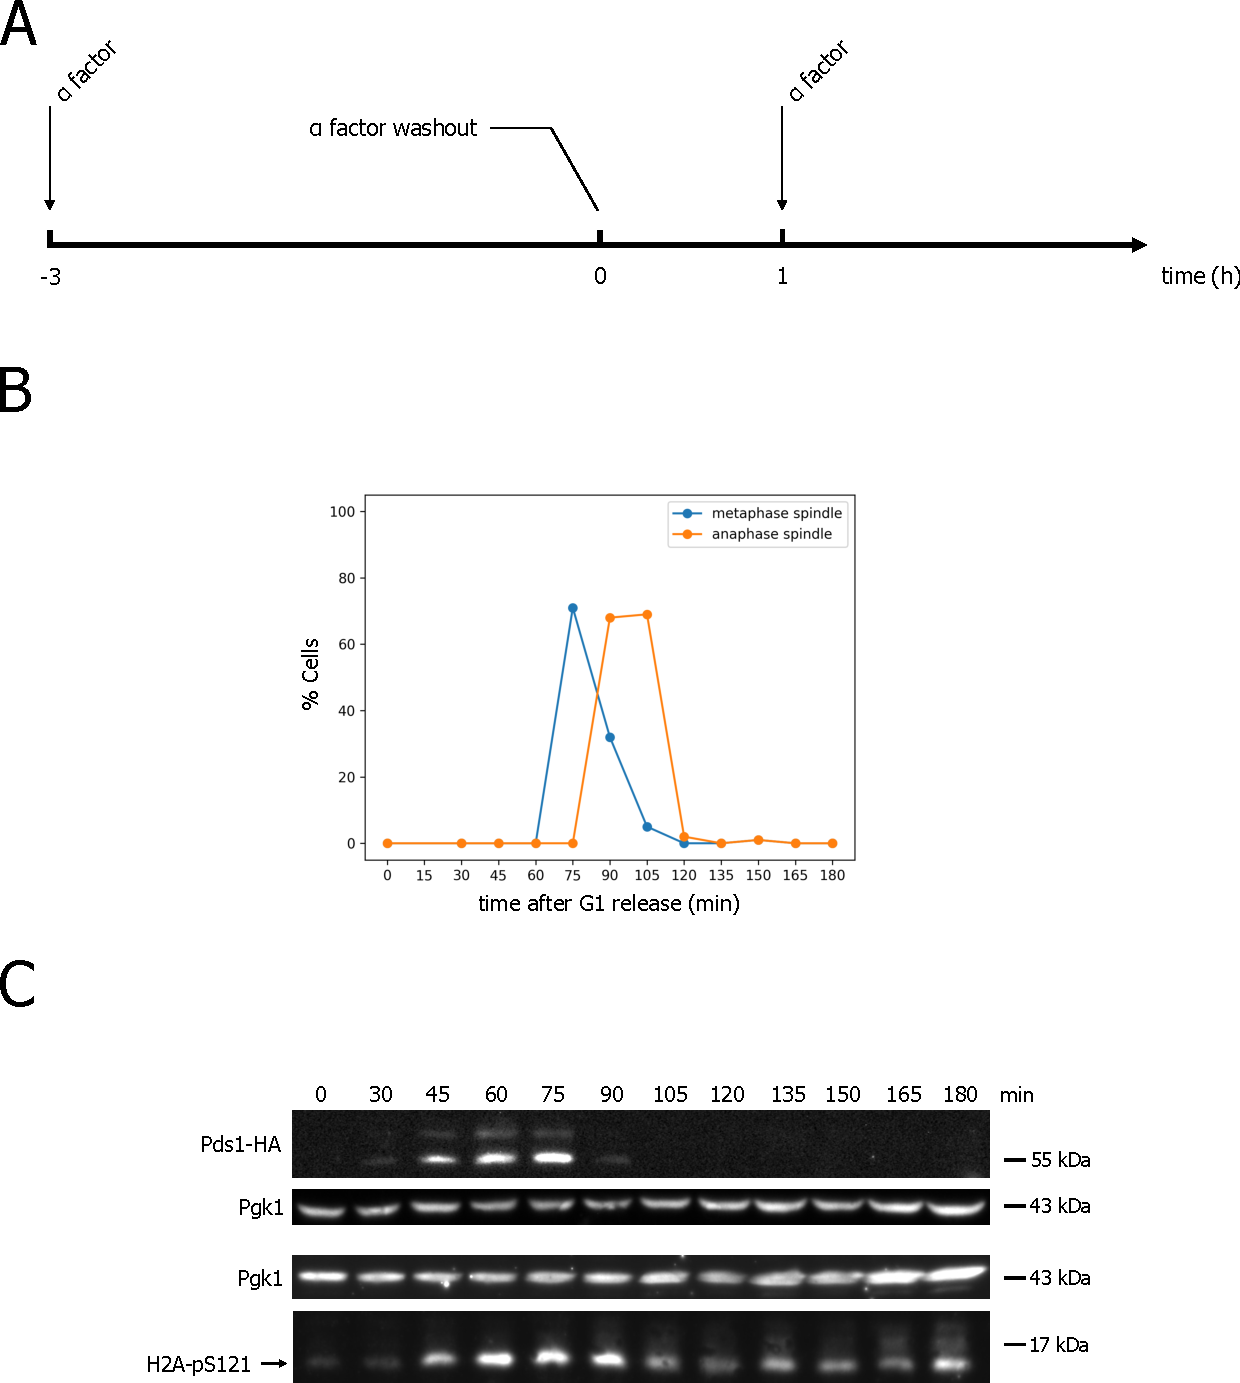
\includegraphics[width=0.9\textwidth]{chapter3/figures/pH2A mitotic time course.pdf}
  \caption[H2A-pS121 level is maintained during metaphase-anaphase transition]{H2A-pS121 level is maintained during metaphase-anaphase transition. (A) Schematics of experimental procedures. (B) The proportion of cells with metaphase or anaphase spindle over time by tubulin IF. (C) Upper: western blotting with anti-HA antibody to detect Pds1 protein. Pgk1 was used as the loading control. Lower: western blotting with anti-H2A-pS121 antibody to detect the phosphorylation status of H2A. Pgk1 was used as the loading control.}
  \label{fig:ph2atimecourse}
\end{figure}

\subsection{Tension re-distributes H2A-pS121 from the centromere to the chromosome arm}

Intuitively, the total level of H2A-pS121 being unaffected by tension contradicts the previous finding that its maintenance requires continued Bub1 and Bub1 is de-localised from the kinetochore upon tension. However, one possibility that can explain both is that de-localised Bub1 reaches and phosphorylates H2A molecules other than the ones localised at the peri-centromere whereas the previously phosphorylated ones at the peri-centromere started to be de-phosphorylated, resulting in a change in the localisation of H2A-pS121 but not the total level. To test this hypothesis, we sought to conduct either IF or ChIP using the H2A-pS121 phospho-specific antibody. Considering the poor specificity of the antibody, I turned to ChIP because it is supposed to provide a better signal-to-noise ratio. 

First, I carried out a test ChIP-qPCR to determine whether the antibody can be used for ChIP as well as the optimal fixing time. tension-less metaphase wild type or \textit{bub1$\Delta$K}, the negative control, cells arrested by nocodazole were fixed for 10, 20, 30 and 60 \si{\minute}. Samples were then subject to ChIP with the anti-H2A-pS121 antibody and qPCR was used to determine the enrichment at the centromere, chromosome arm and peri-centromere of chromosome IV. Signals were detected at the centromere and peri-centromere in wild type but not in \textit{bub1$\Delta$K}, showing that the antibody is capable of ChIP application. Consistent with the localisation in vertebrates by IF experiments \citep{Ricke2012, Kawashima2010a, Liu2013a, Williams2017Bub1Kinetochores, Zhang2020FunctioningMitosis, Liang2019ACells, Lee2008, Liu2015}, H2A-pS121 enrichment is vastly reduced on the chromosome arm in wild type. The fixing time does not seem to be important for this particular experiment. I decided to use 10 \si{\minute} as it should cross-link fewer irrelevant proteins to the DNA in theory and therefore reduce the likelihood of potential artefacts. 

\begin{figure}[htbp]
  \centering
  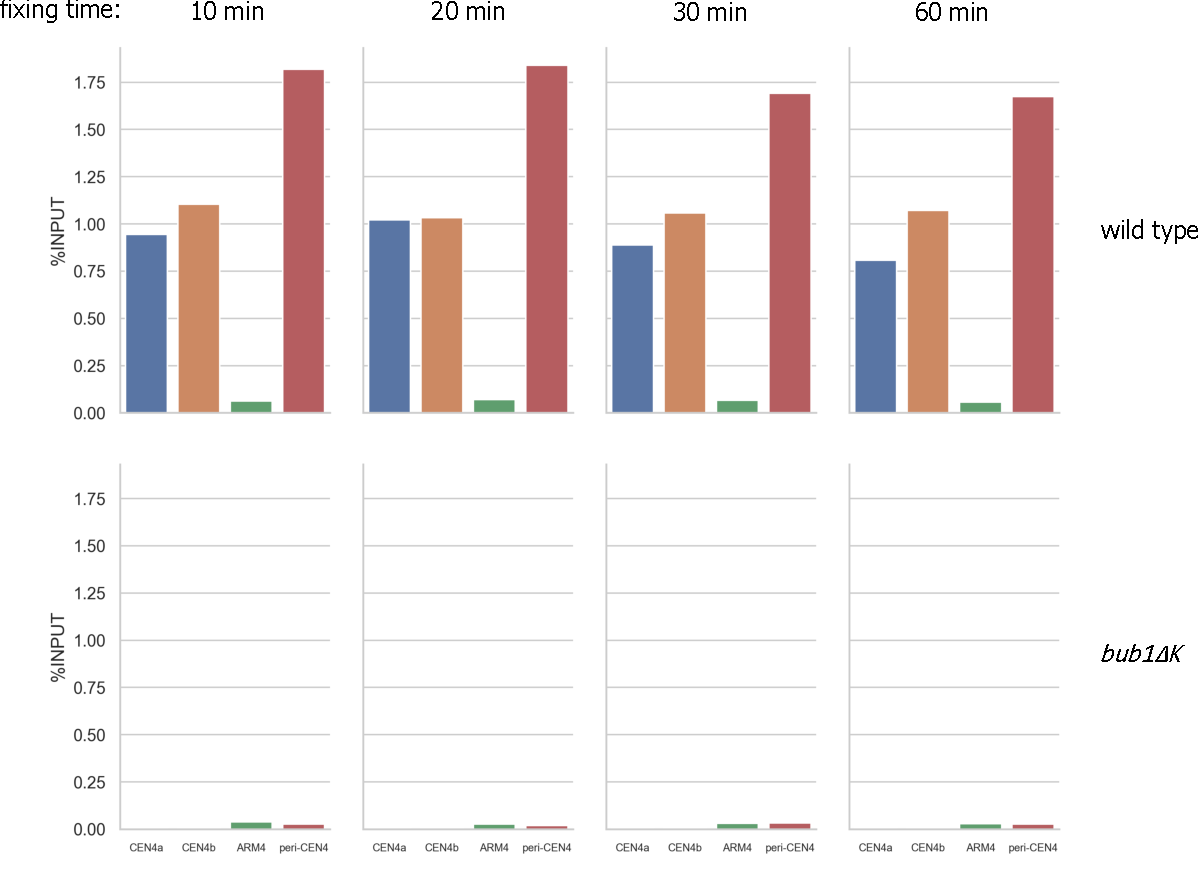
\includegraphics[width=0.9\textwidth]{chapter3/figures/pH2A test ChIP-qPCR.pdf}
  \caption[The H2A-pS121 phospho-specific antibody can be used for ChIP]{The H2A-pS121 phospho-specific antibody can be used for ChIP. Wild type and \textit{bub1$\Delta$K} cells arrested in metaphase without tension were fixed for 10, 20, 30 and 60 minutes, respectively, and subjected to H2A-pS121 ChIP-qPCR at 4 different loci, with two at the centromere, one at chromosome arm and one at the peri-centromere of chromosome IV. }
  \label{fig:ph2atestchipqpcr}
\end{figure}

Next, I conducted a formal H2A-pS121 ChIP-seq experiment. To be able to compare signals between samples, a wet calibration method was used, where the genome from another species, fission yeast in this case, was mixed with the budding yeast genome in the experiment \citep{Hu2015BiologicalChIP-seq}. Wild type cells were arrested in metaphase with or without tension (Figure~\ref{fig:ph2achipseqchecking}A). Tubulin IF indicated that they have good synchronisation. 98\% cells from the tension sample displayed metaphase spindle while none of the cells from the no tension sample showed a spindle (Figure~\ref{fig:ph2achipseqchecking}B). Western blotting was used to examine the level of H2A-pS121 in the two samples. Consistent with the previous results (Subsection~\ref{subsec:totalph2aindten}), both samples showed comparable band intensities (Figure~\ref{fig:ph2achipseqchecking}C). ChIP-processed samples were further checked by qPCR for the enrichment of budding and fission yeast's loci to ensure quality. Similar to the test qPCR, the no tension sample showed high signals at the centromere and peri-centromere but not on the chromosome arm. Consistent with the idea that tension might affect the localisation of H2A-pS121, the tension sample had low signals at all three loci (Figure~\ref{fig:ph2achipseqchecking}D). The amount of fission yeast cells used for calibration is the same between samples. Therefore, it is expected that both of them should give equal enrichment at a given locus. Indeed, the signals were comparable between samples at the centromere core and outer repeat of fission yeast (Figure~\ref{fig:ph2achipseqchecking}E). 

\begin{figure}[htbp]
  \centering
  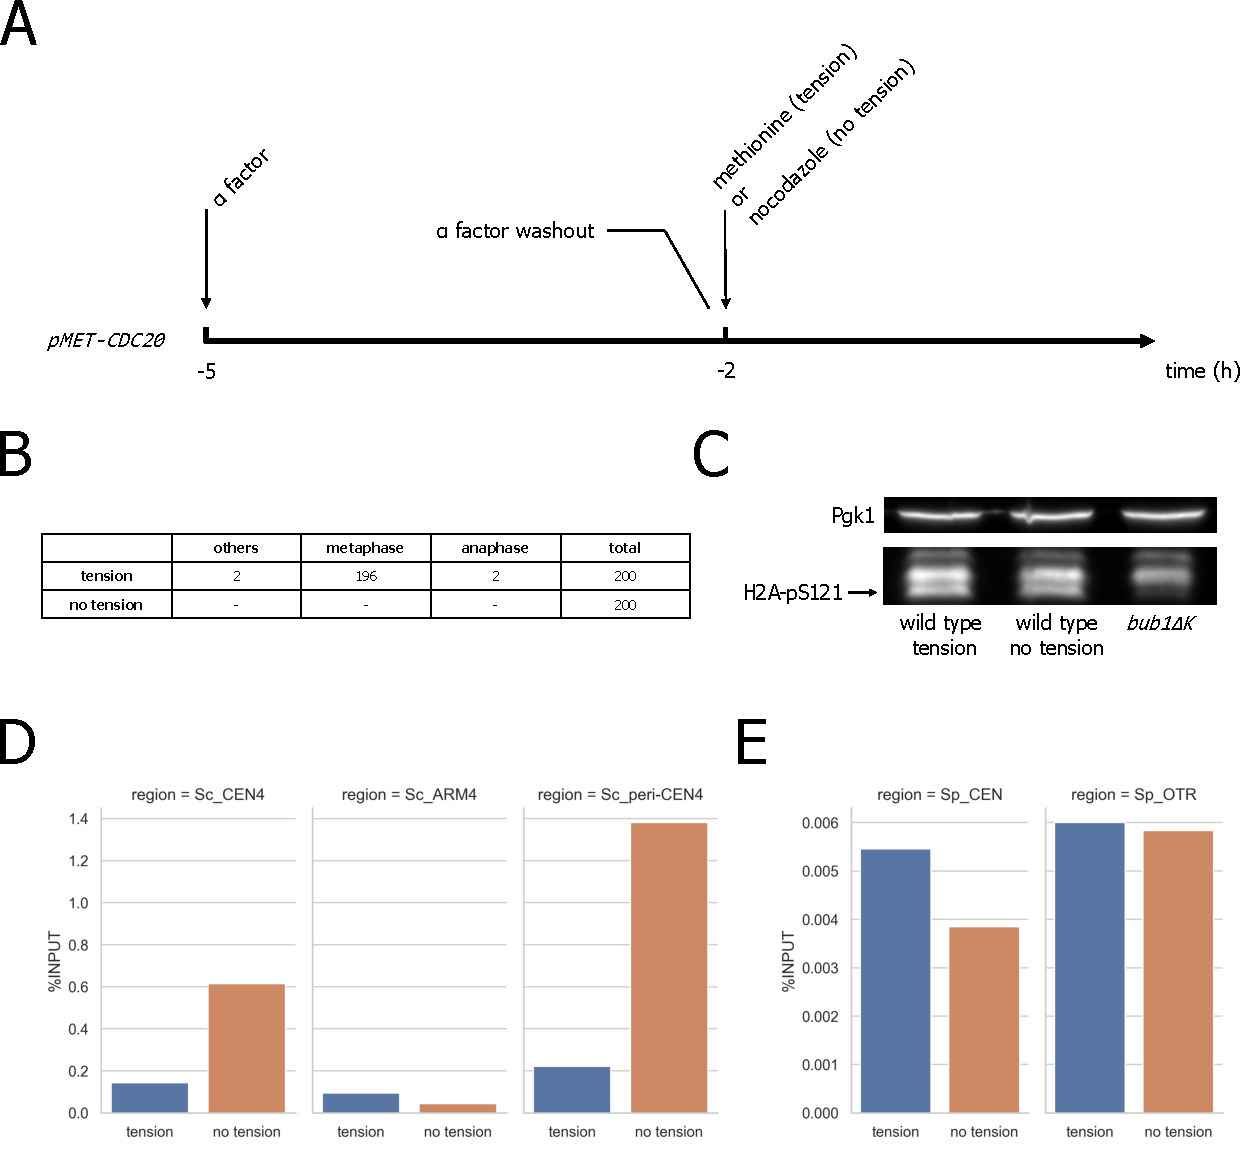
\includegraphics[width=0.9\textwidth]{chapter3/figures/checking.pdf}
  \caption[Quality control of calibrated H2A-pS121 ChIP-seq]{Quality control of calibrated H2A-pS121 ChIP-seq. (A) Schematics of experimental procedures. (B) Spindle morphology count by tubulin IF. (C) Western blotting with anti-H2A-pS121 antibody to detect the phosphorylation status of H2A. Pgk1 was used as the loading control. (D) H2A-pS121 ChIP-qPCR at the chromosome IV centromere, chromosome arm and peri-centromere of \textit{S.cerevisiae}. (E) H2A-pS121 ChIP-qPCR at chromosome I centromere core and outer repeat of \textit{S.pombe}. }
  \label{fig:ph2achipseqchecking}
\end{figure}

With quality control conducted, I proceeded with the ChIP samples and set up sequencing. The enrichment profile of a representative chromosome, chromosome IV, is shown in Figure~\ref{fig:ph2achipseq2nd}A. H2A-pS121 has a bell-shaped distribution at the centromere in both the tension and no tension sample. However, quantitatively, consistent with the result from qPCR, the signals were massively reduced in the tension sample. In contrast, on the chromosome arm, the signals were higher for the tension sample, supporting the hypothesis. This is confirmed by the pile-up of all 16 chromosomes. At centromeres, the signals of the tension sample were about a quarter of that of the no tension sample, whereas, on the arms, the former showed a roughly one-fold increase from the latter (Figure~\ref{fig:ph2achipseq2nd}B). To provide a more quantitative view, I categorised sequencing reads as either at centromeres or on the chromosome arms. Although the total number was similar, only 18\% of reads were assigned to the centromeres in the tension sample while the number is 63\% in the no tension sample (Figure~\ref{fig:ph2achipseq2nd}C). Hence, we concluded that the establishment of tension caused a re-distribution of H2A-pS121 from the centromere to the chromosome arm. 

\begin{figure}[htbp]
  \centering
  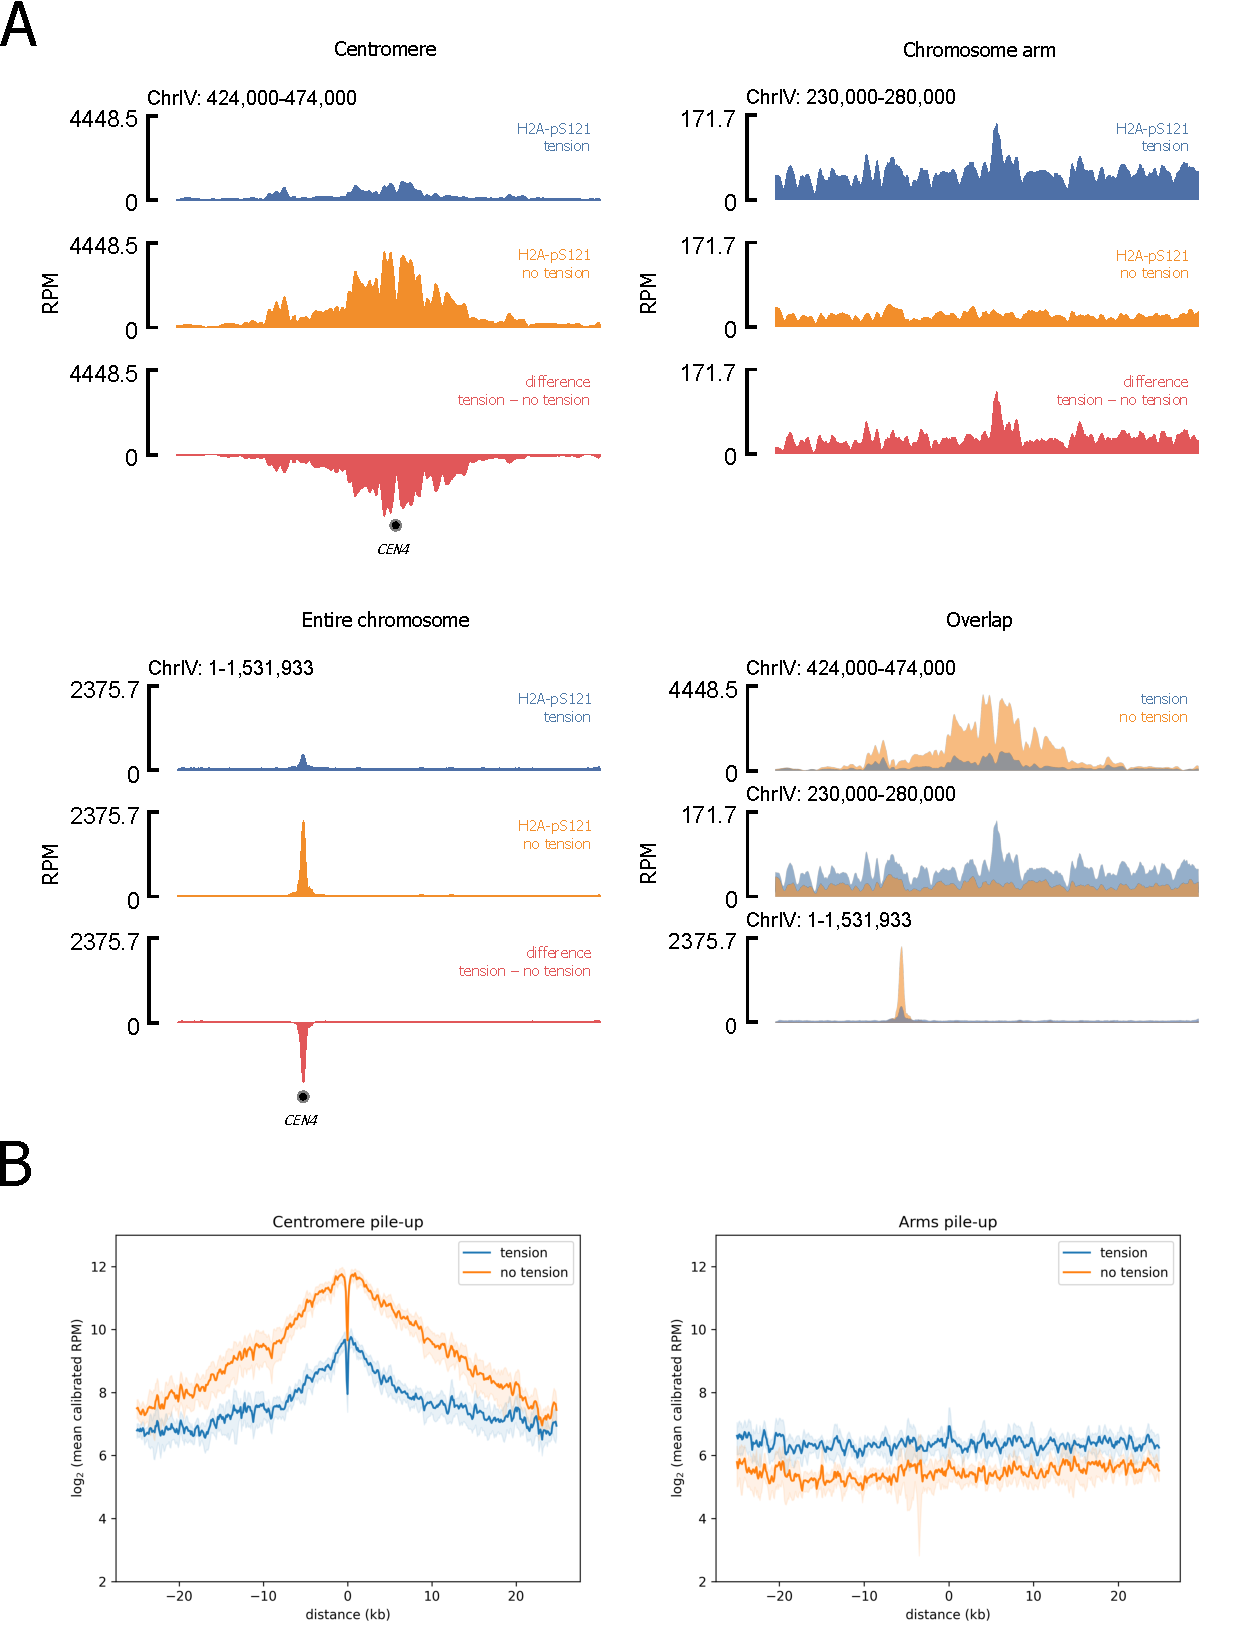
\includegraphics[width=0.9\textwidth]{chapter3/figures/pH2A ChIP-seq_1st.pdf}
\end{figure}

\begin{figure}[t]
  \centering
  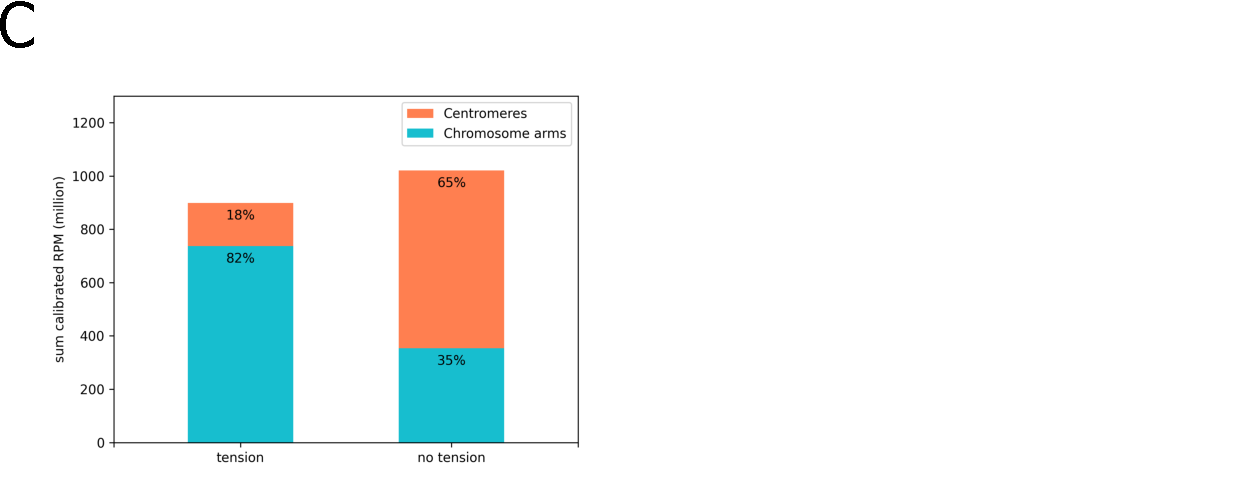
\includegraphics[width=0.9\textwidth]{chapter3/figures/pH2A ChIP-seq_2nd.pdf}
  \caption[H2A-pS121 is re-distributed from centromere to chromosome arm upon the establishment of tension]{H2A-pS121 is re-distributed from centromere to chromosome arm upon the establishment of tension. (A) Calibrated H2A-pS121 ChIP-seq profiles of cells arrested in metaphase with or without tension and their difference (tension - no tension) at the 50kb region around the centromere of chromosome IV (upper left), a 50kb region on the left arm of chromosome IV (upper right) and the entire chromosome IV (bottom left). The overlapped profiles are shown in the bottom right. (B) Pile-up of centromeres and chromosome arms. Left: the 50kb regions around the centromeres of all 16 chromosomes. Right: the 50kb regions around chromosome arms (80kb left to the centromere) of all 16 chromosomes. (C) The number of sequencing reads assigned to centromeres (the 50kb-region flanking the core centromere) or chromosome arms in each sample. }
  \label{fig:ph2achipseq2nd}
\end{figure}

\subsection{Sgo1 cannot be concentrated at the peri-centromere in H2A phospho-mimic mutant}

The re-distribution of H2A-pS121 upon tension points to a possibility that it triggers Sgo1 re-localisation. If it is true, The H2A phospho-mimic mutant whose mark for Sgo1 localisation spreads along the entire chromosome, and thus mimicking the tension situation, should lose its Sgo1 enrichment at peri-centromere in the absence of tension. However, \cite{Nerusheva2014} reported an opposite result and, combined with other results, eventually reached the conclusion that Bub1 has substrates other than H2A important for Sgo1 localisation. Due to a lack of supporting evidence from other species and the difficulty of making H2A mutants in budding yeast, I decided to verify the results by first sequencing the original strains used in the research. Surprisingly, The H2A phospho-mimic mutants turned out to be wild type for the HTA1 locus (Figure~\ref{fig:h2as121dseq}), consistent with the observation that strains with H2A-S121D mutations always show the same phenotype as wild type in the paper. 

\begin{figure}[htbp]
  \centering
  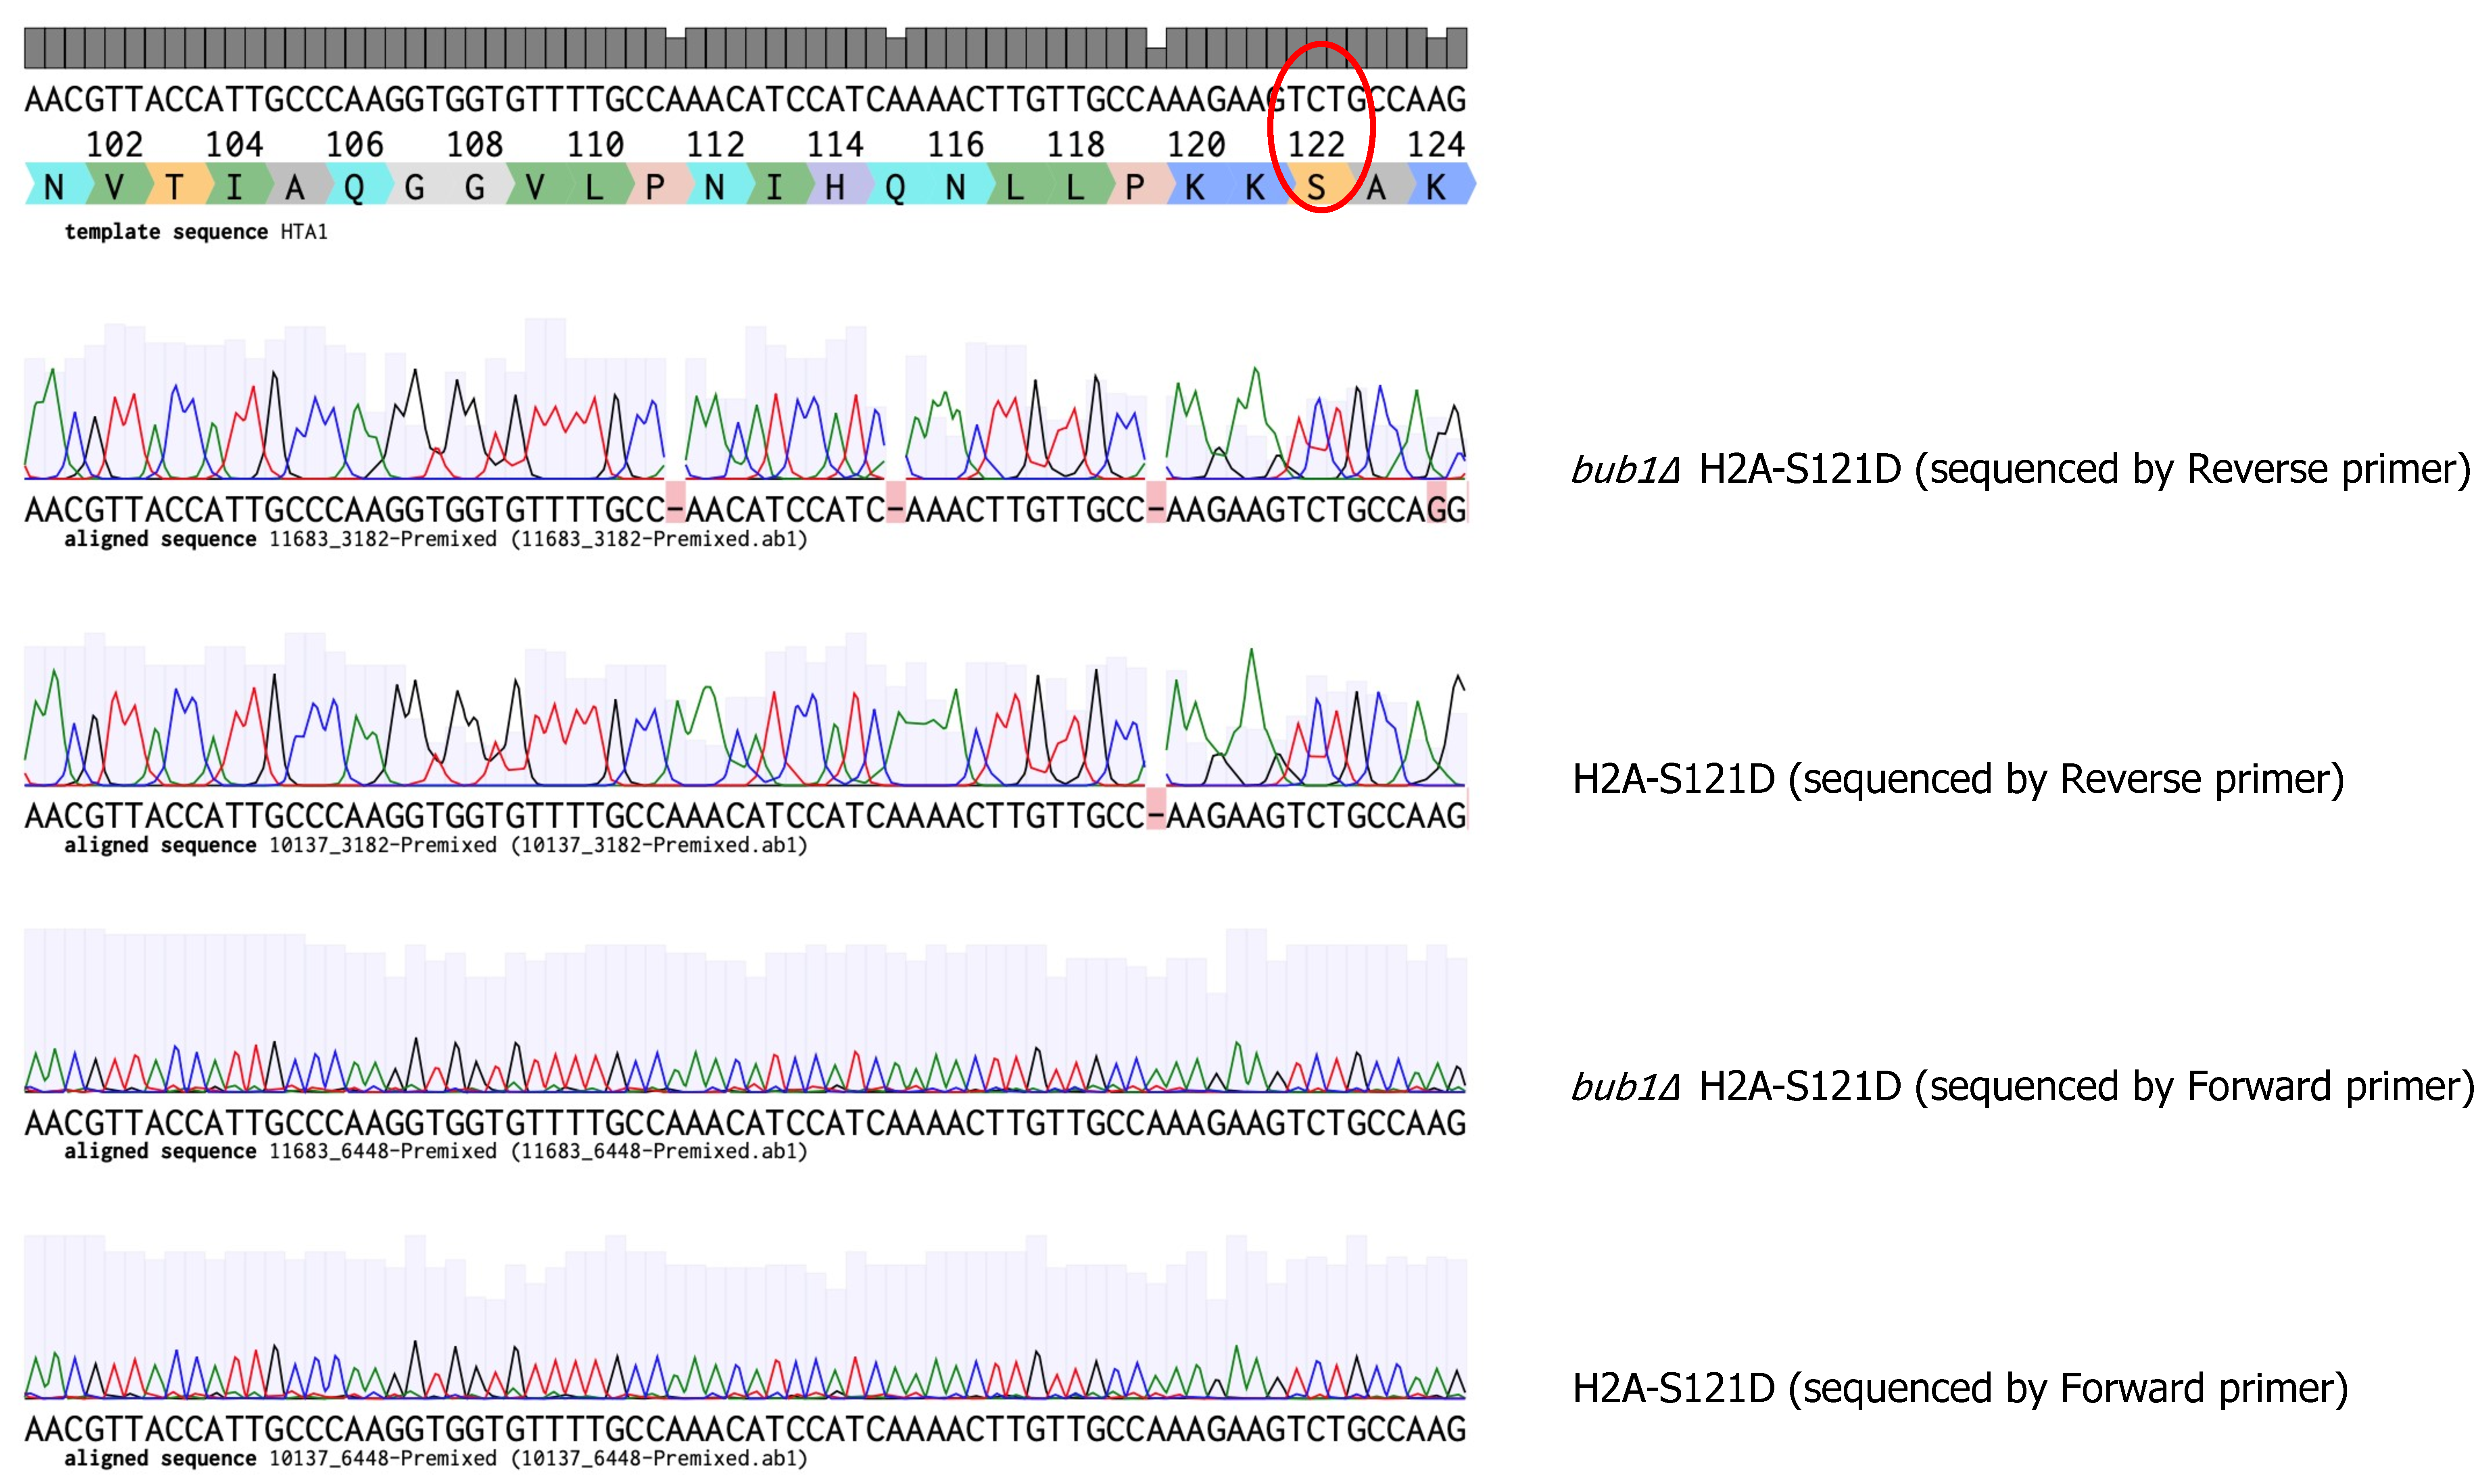
\includegraphics[width=0.9\textwidth]{chapter3/figures/nerusheva_sequencing.pdf}
  \caption[H2A phopho-mimic mutants used in \citep{Nerusheva2014} bear wild type sequence]{Phopho-mimic mutants used in \citep{Nerusheva2014} bear wild type sequence. The red circle indicates the expected mutation site.}
  \label{fig:h2as121dseq}
\end{figure}

To test whether Sgo1 localisation is altered in H2A phospho-mimic mutants, I re-constructed the strain and repeated the Sgo1-6HA ChIP-qPCR experiment by \cite{Nerusheva2014}. The standard cell harvesting procedure comparing tension with no tension conditions was performed on no tag, wild type, H2A-S121A, as a negative control, and H2A-S121D (Figure~\ref{fig:sgo1chiph2amutants}A). Tubulin IF indicated synchronised metaphase arrest in the tension samples and an absence of spindle in the no tension samples (Figure~\ref{fig:sgo1chiph2amutants}B). Western blotting showed comparable Sgo1 expression in wild type, H2A-S121A and H2A-S121D but not in no tag (Figure~\ref{fig:sgo1chiph2amutants}C). Samples then underwent ChIP processing and qPCR was used to determine the enrichment at the chromosome arm, peri-centromere and centromere of chromosome IV (Figure~\ref{fig:sgo1chiph2amutants}D). As expected, Sgo1 exhibited increased association with chromatin at the centromeric/ peri-centromeric region but not on the arm in wild type without tension. However, this increase was abolished in H2A-S121A or H2A-S121D, suggesting Sgo1 cannot be enriched at peri-centromere even in the absence of tension, supporting the idea that the phospho-mimic mutant resembles the scenario with established tension regarding Sgo1 localisation (Figure~\ref{fig:sgo1chiph2amutants}E). 

\begin{figure}[htbp]
  \centering
  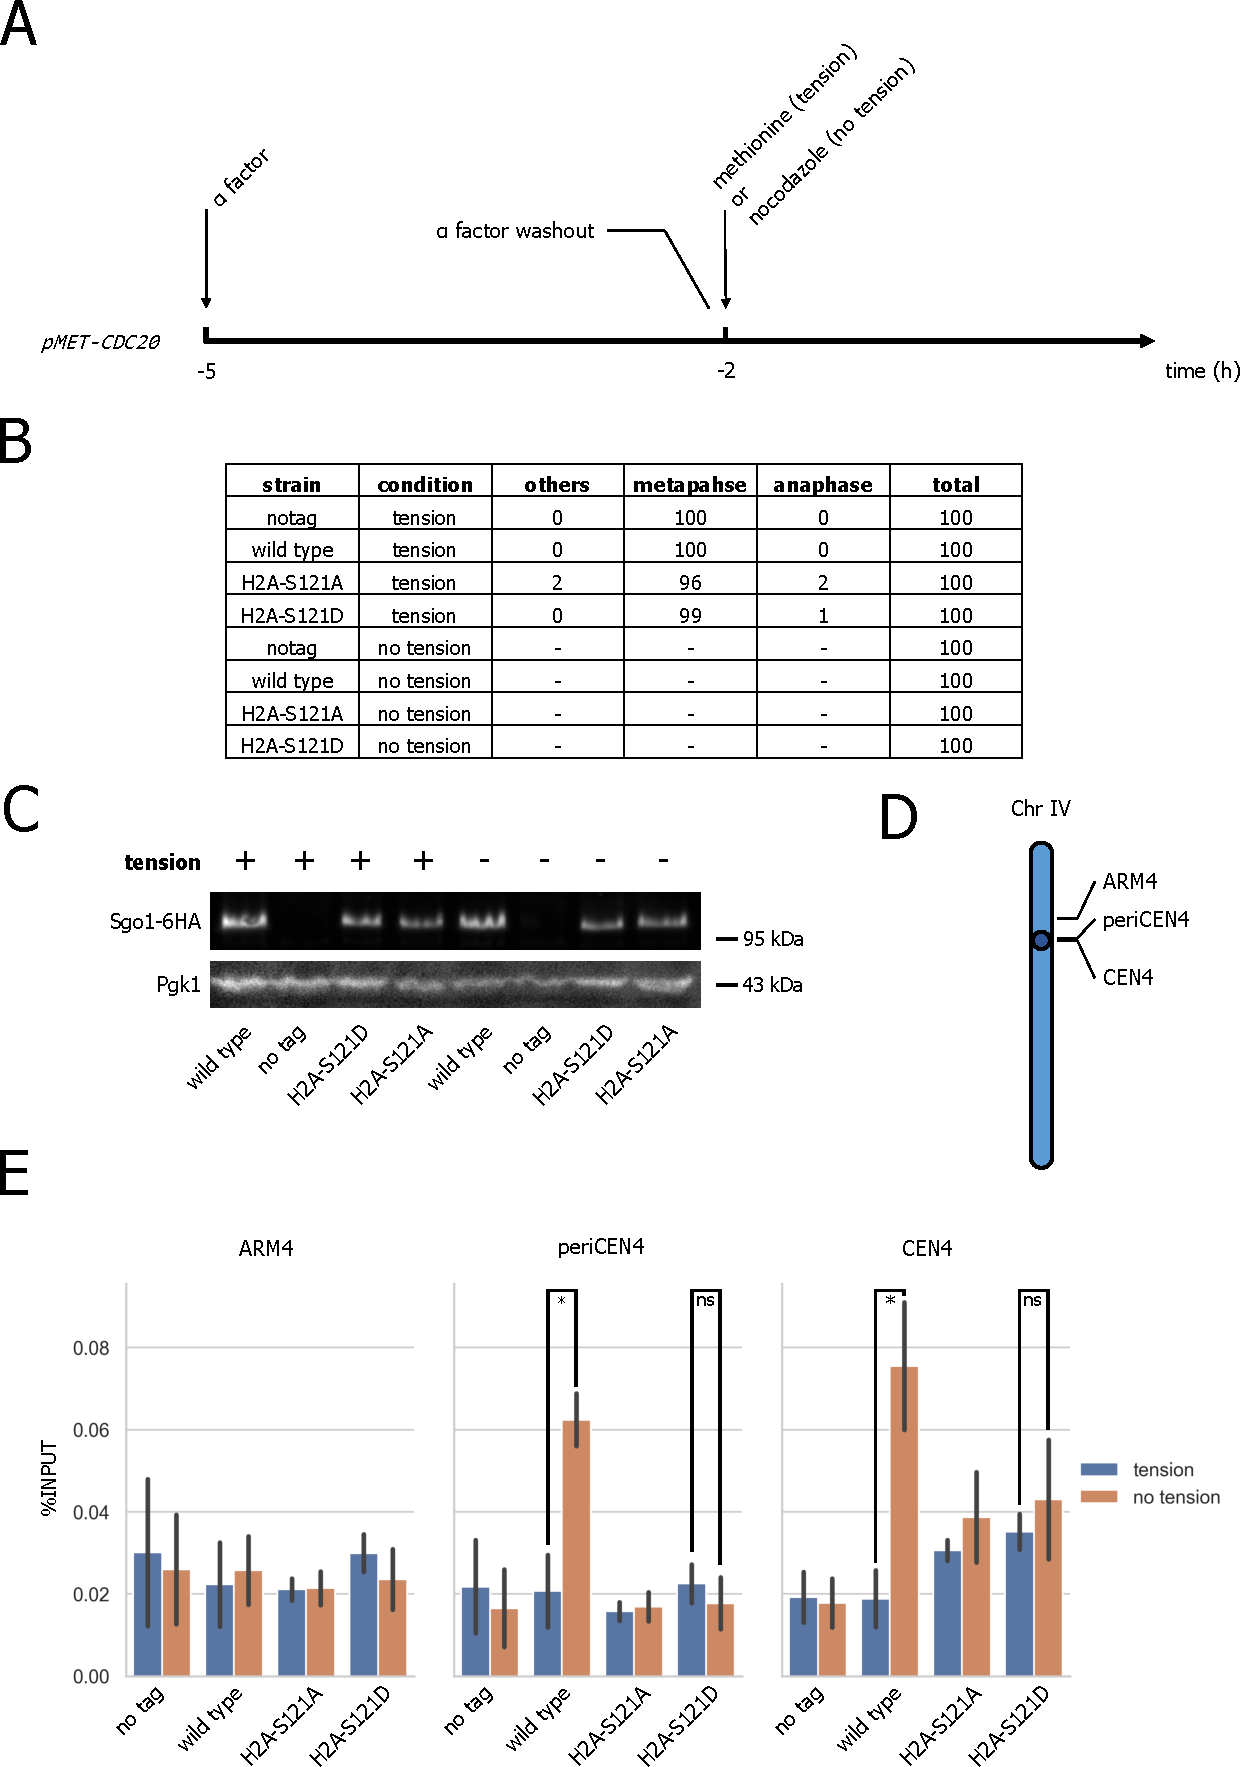
\includegraphics[width=0.9\textwidth]{chapter3/figures/Sgo1 in H2A mutants ChIP.pdf}
  \caption[Sgo1 association with chromatin remains low regardless of tension in H2A phospho-mimic mutant]{Sgo1 association with chromatin remains low regardless of tension in H2A phospho-mimic mutant. (A) Schematics of experimental procedures. (B) Spindle morphology count by tubulin IF. (C) Western blotting with anti-HA antibody to detect the expression level of Sgo1-6HA. Pgk1 was used as the loading control. (D) Schematics showing the locations of loci used for the ChIP-qPCR experiment. (E) Sgo1-6HA ChIP-qPCR on the chromosome arm, the peri-centromere and the core centromere of chromosome IV. The mean of 3 experimental repeats is shown, with the error bar representing standard error. The two-tailed independent t-test is used to calculate statistical significance. (*) P<0.05; (ns) not significant.}
  \label{fig:sgo1chiph2amutants}
\end{figure}

Due to the apparent contradiction with the previous result, I sought to validate the result with microscopy. Therefore, I constructed H2A mutants bearing genetic constructs for imaging, \textit{SGO1-EGFP MTW1-tdTomato}. Cells were imaged following the standard approach of synchronised G1 to metaphase live-cell imaging (Figure~\ref{fig:sgo1imagingh2amutants}A). Unlike wild type, where Sgo1-EGFP appeared as foci at least once in the cell cycle, both of the H2A phospho-mutants could only show Sgo1-EGFP as a 'cloud' signal (Figure~\ref{fig:sgo1imagingh2amutants}B and C). Again, this 'cloud' signal resembles what it looks like in wild type after the establishment of tension, judged by the separation of kinetochore foci. Western blotting showed similar Sgo1 expression levels in the three strains used, ruling out the possibility that the loss of Sgo1-EGFP foci is because of reduced protein abundance (Figure~\ref{fig:sgo1imagingh2amutants}D). Therefore, I concluded that Sgo1 cannot be concentrated at the peri-centromere in H2A phospho-mimic mutant. 

\begin{figure}[htbp]
  \centering
  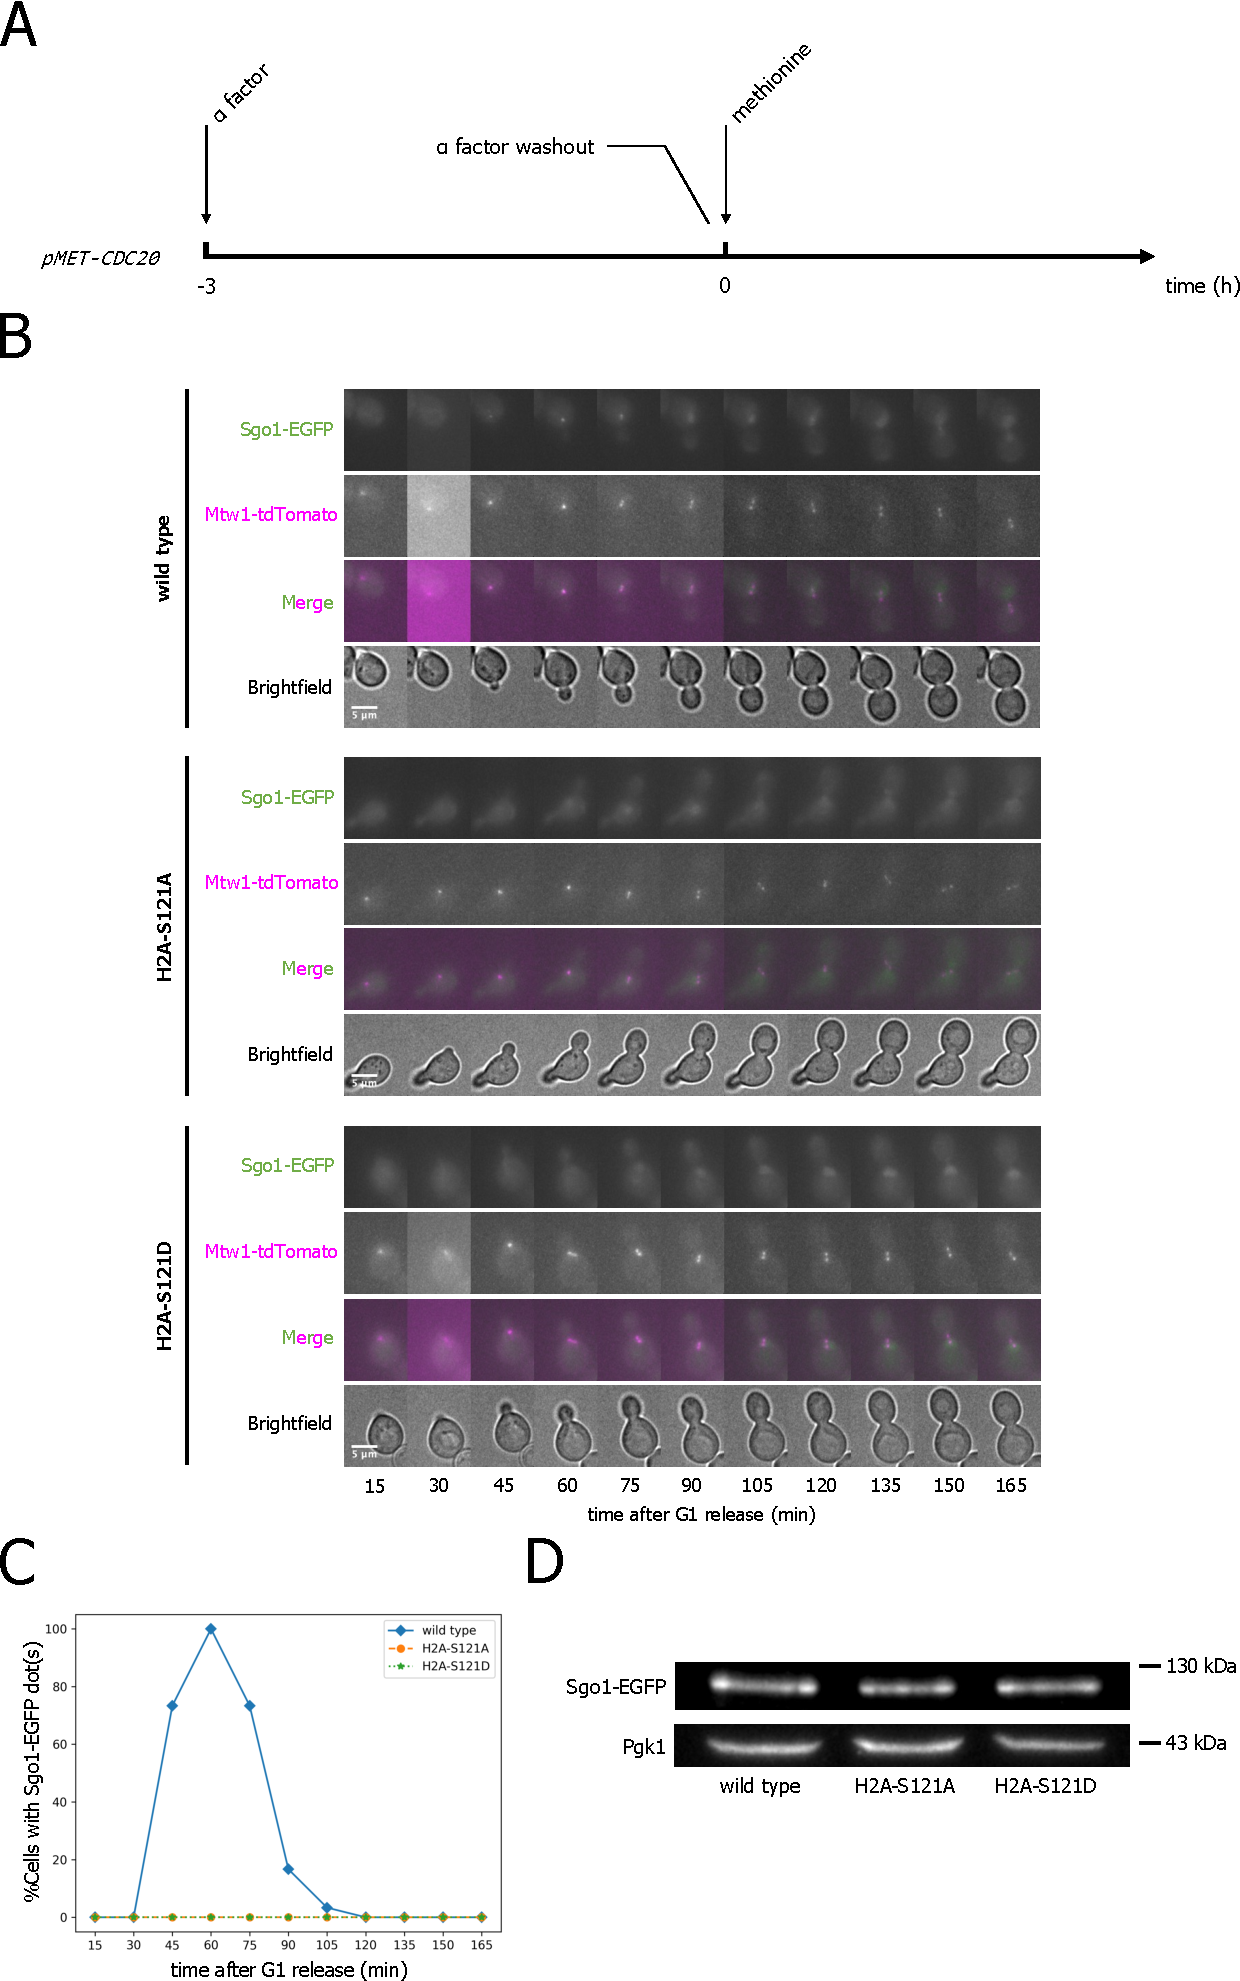
\includegraphics[width=0.9\textwidth]{chapter3/figures/Sgo1 in H2A mutants imaging.pdf}
  \caption[Sgo1 peri-centromere enrichment is abolished in H2A phospho-mimic mutant]{Sgo1 peri-centromere enrichment is abolished in H2A phospho-mimic mutant. (A) Schematics of experimental procedures. (B) Montages of representative time-lapse imaging. (C) N=30 cells for each strain were followed over time and quantified. The percentage of cells with Sgo1-EGFP foci was shown as a function of time. (D) Western blotting on cells arrested in metaphase without tension using anti-GFP antibody to detect the expression level of Sgo1-EGFP. Pgk1 was used as the loading control.}
  \label{fig:sgo1imagingh2amutants}
\end{figure}

\subsection{\textit{sgo1$\Delta$} suppresses the growth defect of PP1 temperature-sensitive mutants at their restrictive temperatures}

The working model predicts the existence of one or more phosphatases constantly de-phosphorylating H2A-pS121. We hypothesised PP1 to be one possible candidate. PP1 is a major serine/ threonine phosphatase ubiquitous in eukaryotes and regulates a large number of cellular processes, including SAC silencing and tension sensing \citep{Shi2009Serine/threonineStructure, Cannon2010FunctionCerevisiae, Pinsky2009ProteinYeast, Pinsky2006Glc7/proteinGlc7, London2012, Meadows2011SpindleMotors, Nijenhuis2014NegativeSignal, Rosenberg2011KNL1/Spc105Checkpoint, Liu2010RegulatedKinase, Posch2010Sds22Mitosis, Jin2013TheAttachment}. A functional PP1 enzyme usually consists of a catalytic subunit, which is highly conserved across species, and a regulatory subunit controlling the localisation, substrate specificity, or activity of the catalytic subunit or serves as the substrate itself. The recognition of the catalytic subunit is majorly through the RxVxF motif, and is often accompanied by an additional MyPhoNE or SILK motif \citep{Hendrickx2009DockingPhosphatase-1}. Budding yeast has a single gene encoding the catalytic subunit called \textit{GLC7} \citep{Cannon2010FunctionCerevisiae}. Consistent with its role in SAC silencing, inactivating Glc7 by using temperature-sensitive mutants results in prolonged metaphase arrest and therefore inviability \citep{Andrews2000TypeCerevisiae, MacKelvie1995ThePhosphatase}. 

I started by checking if \textit{SGO1} has genetic interaction with \textit{GLC7}. It has been shown that not allowing Sgo1 re-localisation upon tension by tethering Sgo1 to the kinetochore also arrests cells in metaphase \citep{Su2021SumoylationAnaphase}. If PP1 is the phosphatase that de-phosphorylates H2A-pS121, the growth defect from Glc7 inactivation could be partially attributed to impaired Sgo1 removal. Hence, depleting Sgo1 should be able to relieve it. To test this idea, I constructed double mutants of \textit{sgo1$\Delta$} and \textit{GLC7} temperature-sensitive alleles, either \textit{glc7-10} or \textit{glc7-12}, and carried out spot assay. As reported in previous research \citep{MacKelvie1995ThePhosphatase, Andrews2000TypeCerevisiae}, at their respective restrictive temperatures, 37 \si{\celsius} for \textit{glc7-10} and 34 \si{\celsius} for \textit{glc7-12}, both single mutants were inviable. However, when combined with \textit{sgo1$\Delta$} as double mutants, both strains showed a slight increase in viability (Figure~\ref{fig:growthassay}A), supporting the idea that PP1 is involved in Sgo1 re-localisation from the peri-centromere. 

To verify this result, I wanted to test if \textit{bub1$\Delta$K} mutant, which has unphosphorylated H2A and cannot localise its Sgo1, could phenocopy \textit{sgo1$\Delta$} in restoring the viability of \textit{GLC7} temperature-sensitive mutants. To our surprise, the double mutants indicated the same, if not less, viability compared to \textit{glc7-10} or \textit{glc7-12} single mutant (Figure~\ref{fig:growthassay}B). This finding argues against the hypothesis. However, it has been reported in humans that Bub1 kinase activity is required for cellular processes other than localising Sgo1 \citep{Tang2004, Nyati2015TheSignaling, Li2018TheReplication, Zhang2020FunctioningMitosis}. We reasoned that the loss of other functions of Bub1 kinase might outweigh the benefit of removing Sgo1 from the peri-centromere in the double mutants here. 

\begin{figure}[htbp]
  \centering
  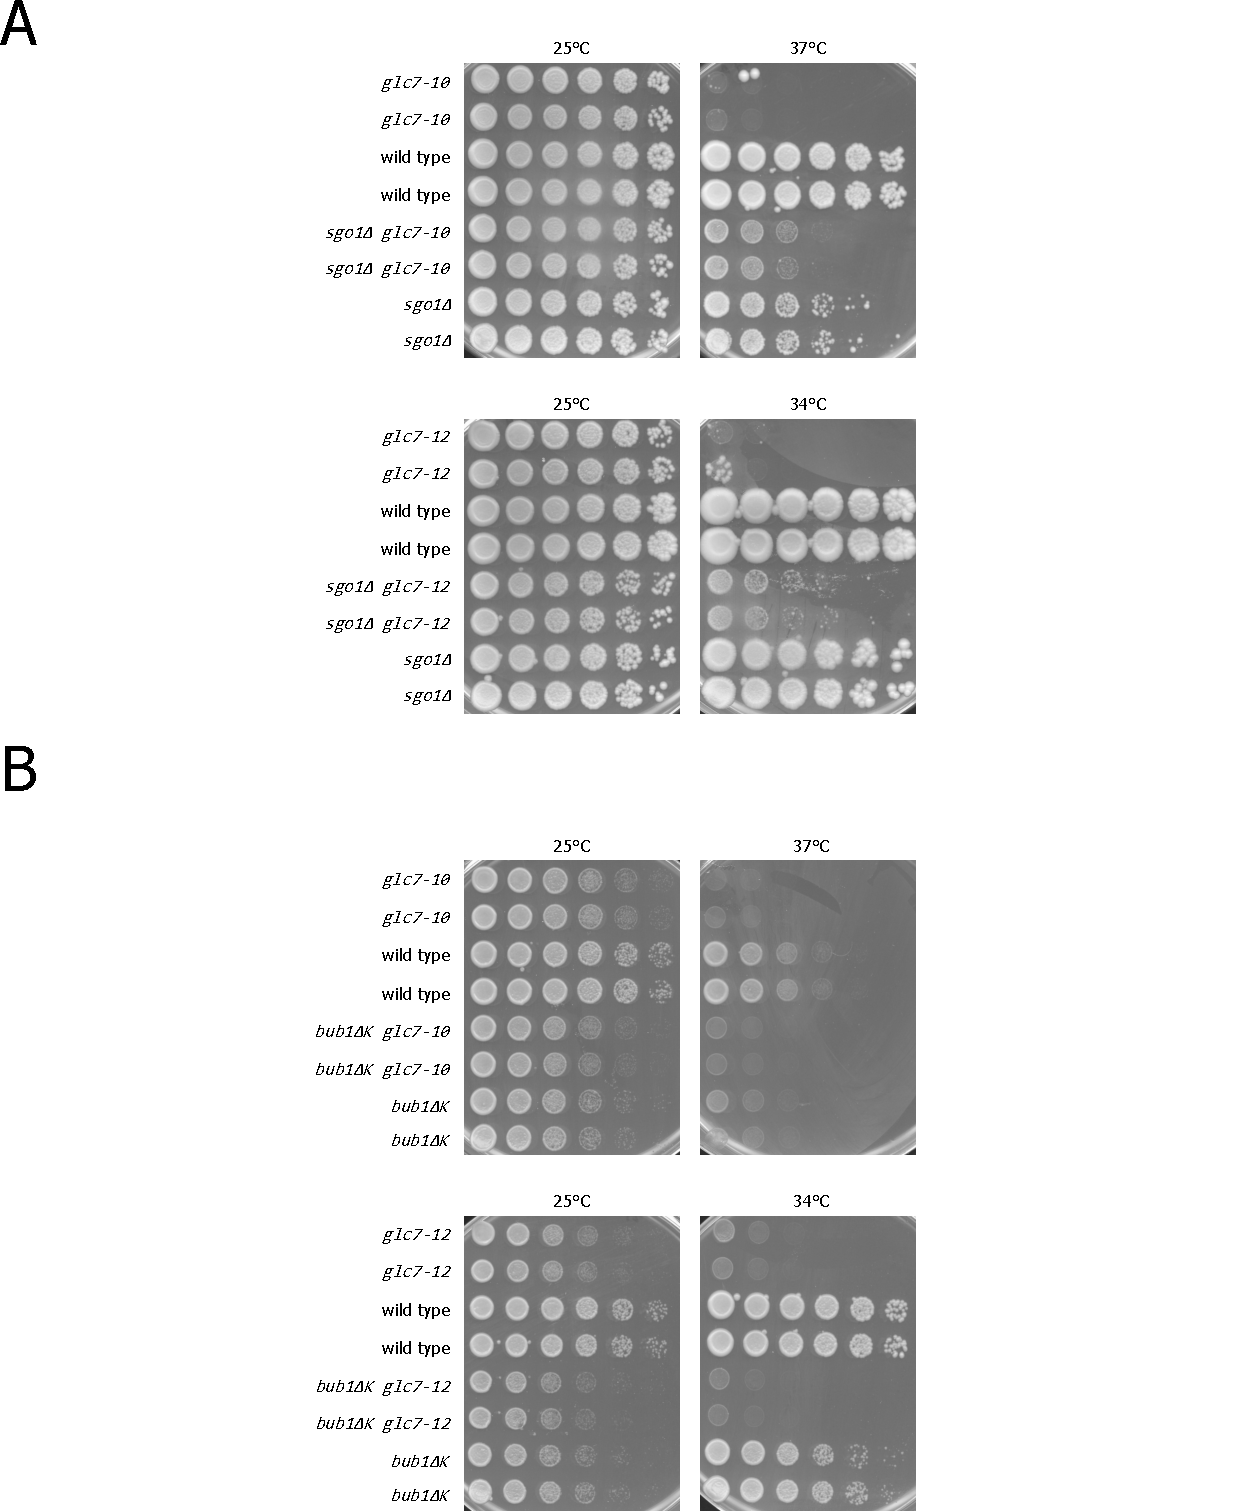
\includegraphics[width=0.9\textwidth]{chapter3/figures/glc7 mutants growth assaay.pdf}
  \caption[\textit{sgo1$\Delta$} but not \textit{bub1$\Delta$K} suppresses the temperature sensitivity of \textit{glc7-10} and \textit{glc7-12} mutant]{\textit{sgo1$\Delta$} but not \textit{bub1$\Delta$K} suppresses the temperature sensitivity of \textit{glc7-10} and \textit{glc7-12} mutant. (A) Serial dilutions of wild type, \textit{sgo1$\Delta$} and \textit{glc7-10} or \textit{glc7-12} single and double mutants spotted on rich medium at room or restrictive temperature. (B) Serial dilutions of wild type, \textit{bub1$\Delta$K} and \textit{glc7-10} or \textit{glc7-12} single and double mutants spotted on rich medium at room or restrictive temperature. The duplications represent technical repeats. }
  \label{fig:growthassay}
\end{figure}

\nomenclature{PP1}{Protein Phosphatase 1}

\subsection{PP1 is required for Sgo1 re-localization}

With the results from the spot assay, I wanted to study the localisation of Sgo1 upon Glc7 inactivation to test whether PP1 is required for Sgo1 removal from the peri-centromere. I first constructed the strain with genetic constructs for Sgo1 imaging (\textit{SGO1-EGFP MTW1-tdTomato pMET-CDC20}) and \textit{glc7-12}, whose restrictive temperature is lower than \textit{glc7-10} and thus might be more compatible with live-cell imaging. the standard G1 to metaphase arrest with tension imaging was conducted except that cells were shifted to 34 \si{\celsius} immediately after G1 release to inactivate PP1 (Figure~\ref{fig:sgo1glc712}A). 

In terms of the inter-kinetochore distance, wild type was similar as in the previous experiments, albeit escaped the arrest induced by Cdc20 depletion near the end of imaging, possibly due to the elevated temperature. Whereas in \textit{glc7-12}, it was stabilised at a much shorter distance, around 0.5 \si{\micro\metre}, over time (Figure~\ref{fig:sgo1glc712}B and C), consistent with the previous report that \textit{glc7-12} cells were arrested in metaphase with short spindles \citep{MacKelvie1995ThePhosphatase}. Interestingly, similar to some of other \textit{GLC7} mutants \citep{Black1995A1, Andrews2000TypeCerevisiae}, many \textit{glc7-12} cells showed elongated bud morphology. The elevated temperature reduced the imaging quality yet the Sgo1-EGFP foci remained distinguishable from the background. Strikingly, in contrast to wild type, Sgo1-EGFP was retained as foci till the end of the experiment in \textit{glc7-12}. Quantification showed that the percentage of \textit{glc7-12} having Sgo1-EGFP foci increased over time and reached nearly 100\% (Figure~\ref{fig:sgo1glc712}B and C), suggesting that Sgo1 cannot be de-localised from the peri-centromere without functional PP1. 

The shortened inter-kinetochore distance in \textit{glc7-12} raised the possibility that Sgo1 is not re-localised because of reduced tension. To test if enough tension was generated in \textit{glc7-12}, I sought to compare the inter-kinetochore distance at which Sgo1 is removed in wild type and the maximum that \textit{glc7-12} could reach. Technically, for individual wild type cell, I identified the first frame that Sgo1-EGFP foci disappeared and recorded its distance between Mtw1-tdTomato foci, which I referred to as wild type$_{removal}$; while for individual \textit{glc7-12} cell, I followed it over time and selected the longest distance its Mtw1-tdTomato foci ever separated, which I named as \textit{glc7-12}$_{maximum}$. As shown in Figure~\ref{fig:sgo1glc712}D, \textit{glc7-12}$_{maximum}$ was slightly larger than wild type$_{removal}$, indicating that \textit{glc7-12} had reached inter-kinetochore distances where Sgo1 is supposed to be de-localised. Therefore, I concluded that the retention of Sgo1 in \textit{glc7-12} cannot be simply explained by the reduced tension. Western blotting further confirmed that this retention is not due to an altered Sgo1-EGFP expression in \textit{glc7-12} (Figure~\ref{fig:sgo1glc712}E). 

\begin{figure}[htbp]
  \centering
  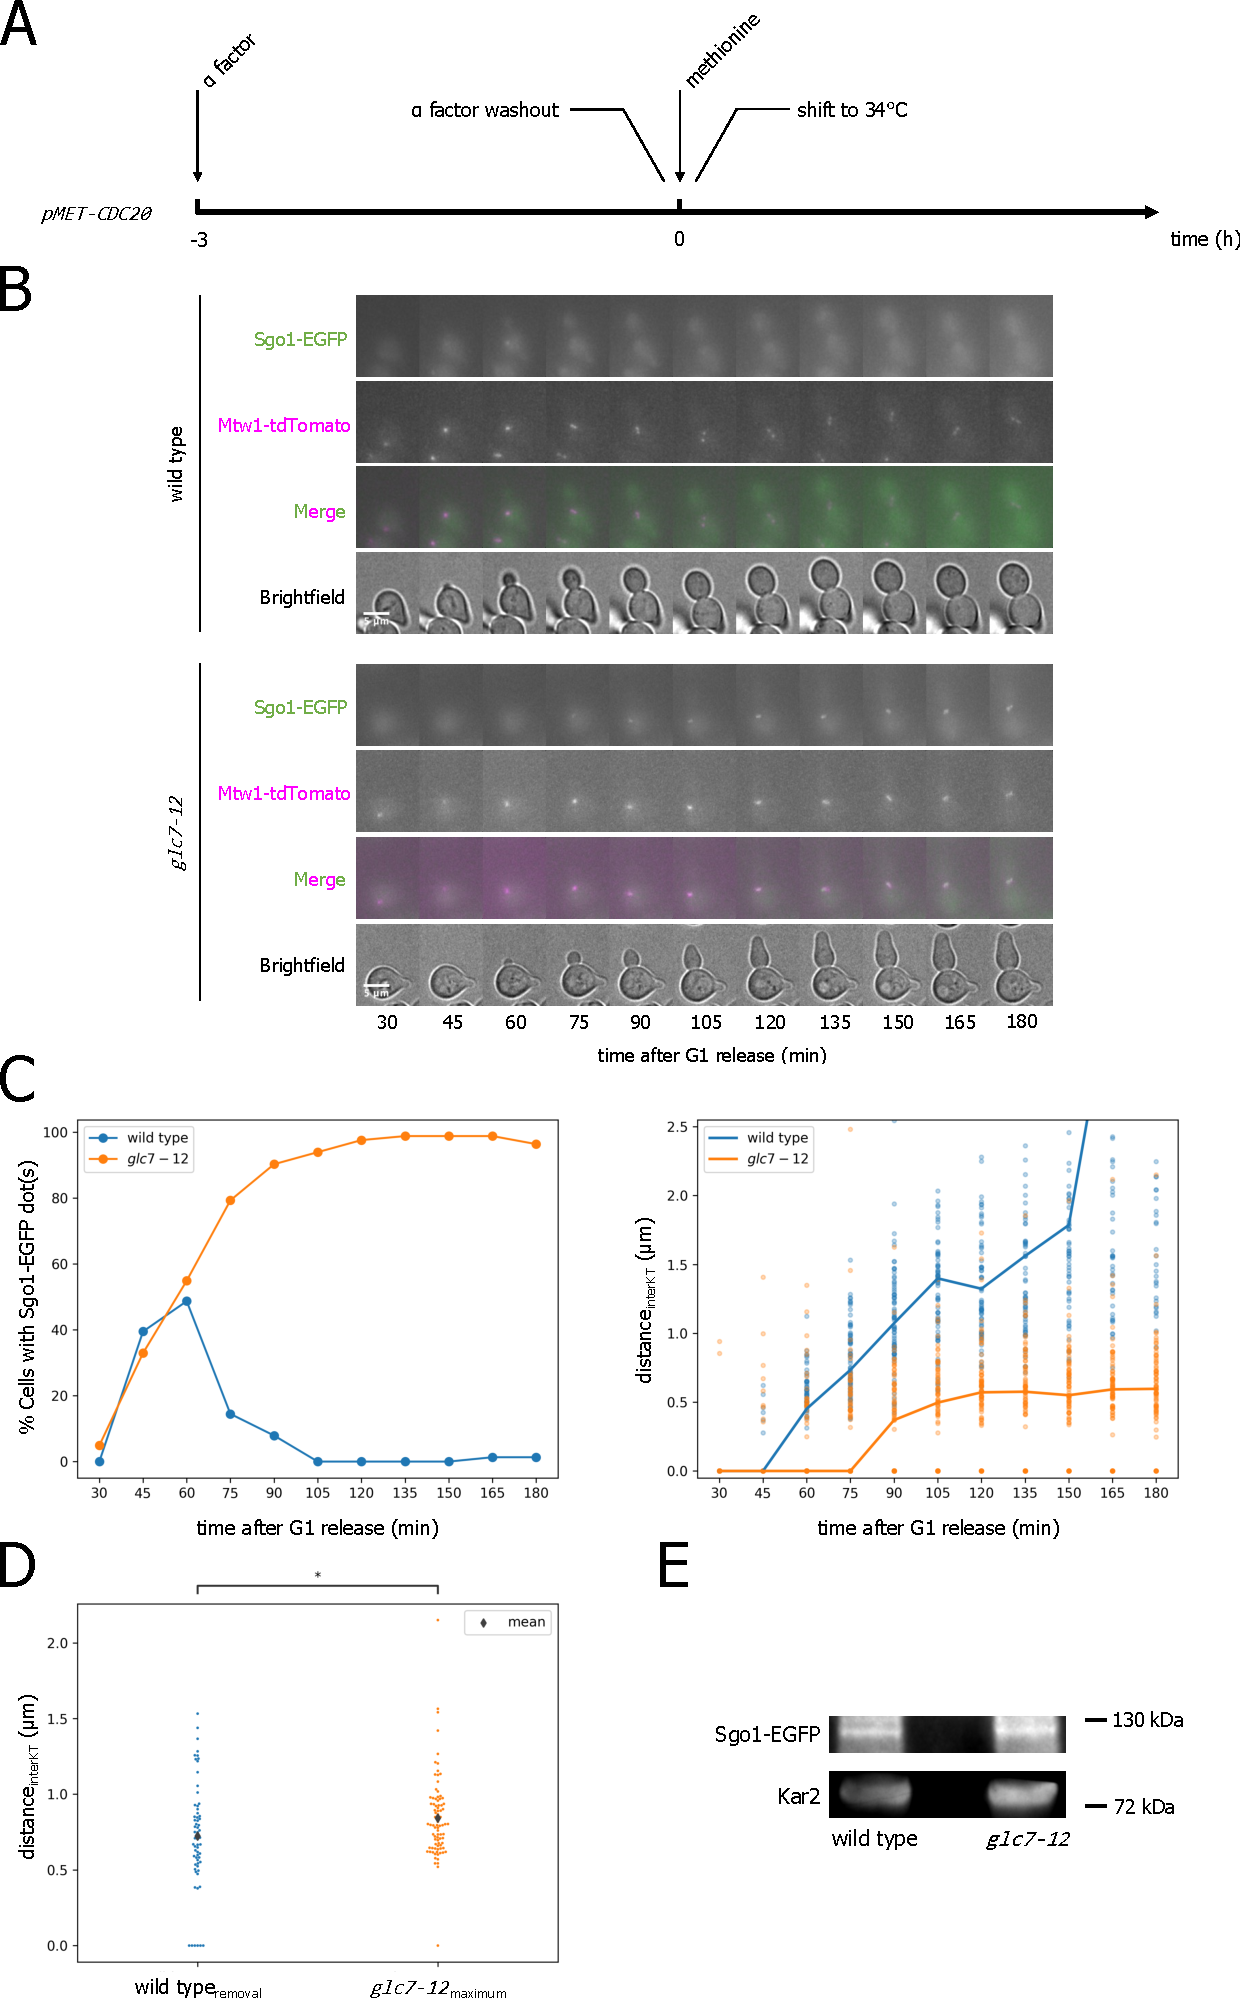
\includegraphics[width=0.9\textwidth]{chapter3/figures/Sgo1 glc7-12.pdf}
  \caption[Sgo1 is not de-localised from peri-centromere in \textit{glc7-12} at restrictive temperature]{Sgo1 is not de-localised from peri-centromere in \textit{glc7-12} at restrictive temperature. (A) Schematics of experimental procedures. (B) Montages of representative time-lapse imaging. (C) N=100 cells for each strain were followed over time and quantified. Top panel: the percentage of cells with Sgo1-EGFP foci was shown as a function of time. Bottom panel: median inter-kinetochore distance as a function of time. Individual data points are shown as dots. (D) Comparison between the inter-kinetochore distance at which Sgo1 is removed in wild type (wild type$_{removal}$) and the maximum that \textit{glc7-12} could reach (\textit{glc7-12}$_{maximum}$). The two-tailed independent t-test was used to calculate statistical significance. (*) P<0.05 (E) Western blotting on cells arrested in metaphase without tension using anti-GFP antibody to detect the expression level of Sgo1-EGFP. Kar2 was used as the loading control.}
  \label{fig:sgo1glc712}
\end{figure}

To verify the result, I repeated the experiment in \textit{glc7-10} background (Figure~\ref{fig:sgo1glc710}A). Consistently, Sgo1-EGFP was maintained as foci within the scope of the experiment (Figure~\ref{fig:sgo1glc710}B), supporting the conclusion that PP1 is required for Sgo1 re-localisation. Notably, this experiment's imaging quality was better compared to the one for \textit{glc7-12}. This is unexpected as it was conducted at an even higher temperature. I suspect it might be related to the fact there is immersion oil optimised for imaging at 37 \si{\celsius} but not 34 \si{\celsius}. 

\begin{figure}[htbp]
  \centering
  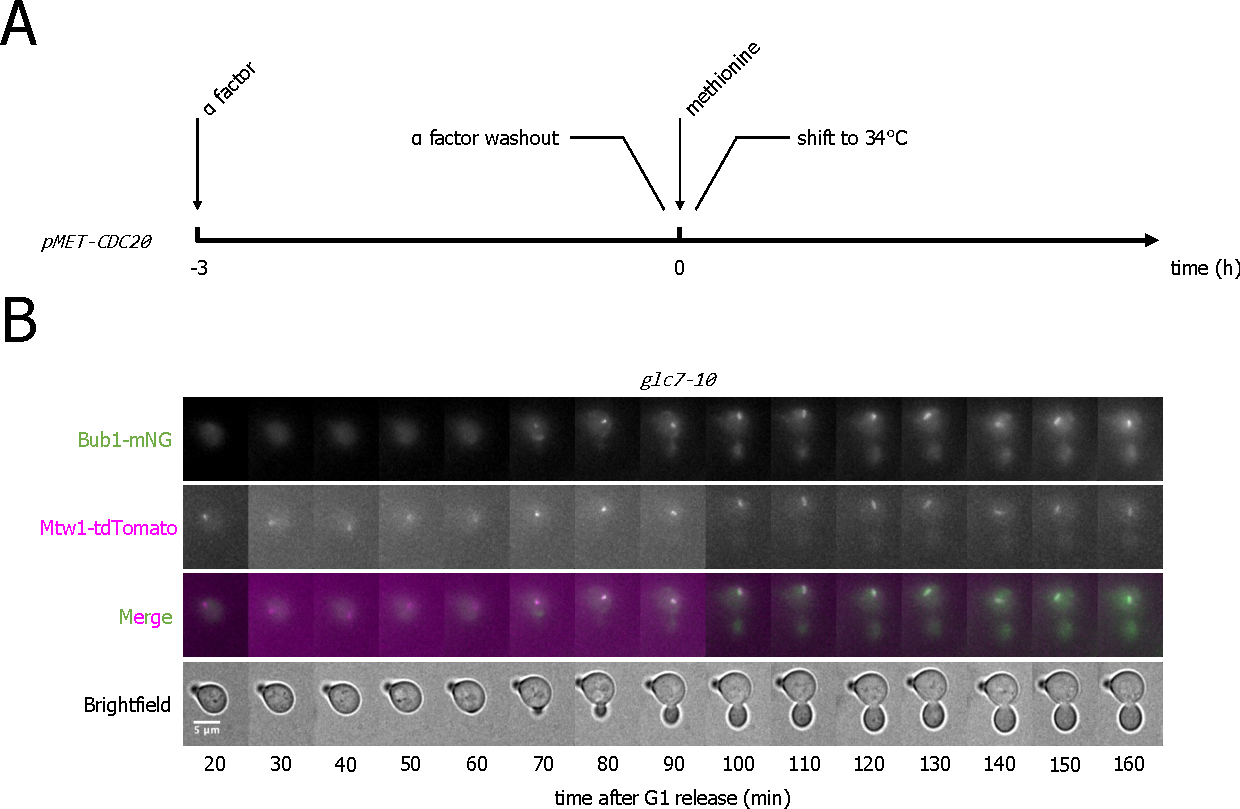
\includegraphics[width=0.9\textwidth]{chapter3/figures/Sgo1 glc7-10.pdf}
  \caption[Sgo1 is not de-localised from peri-centromere in \textit{glc7-10} at restrictive temperature]{Sgo1 is not de-localised from peri-centromere in \textit{glc7-10} at restrictive temperature. (A) Schematics of experimental procedures. (B) Montages of representative time-lapse imaging.}
  \label{fig:sgo1glc710}
\end{figure}

\subsection{PP1-inactivation-caused retention of Sgo1 depends on Bub1}

Next, we wondered whether PP1 is the phosphatase counteracting Bub1 in terms of localising Sgo1. If so, we expected that Sgo1 localisation should be maintained in the absence of both Bub1 and PP1 (Figure~\ref{fig:bub1aidglc712}B). To test this idea, I repeated the 
Bub1 depletion experiment of Figure~\ref{fig:bub1aid} but in the \textit{glc7-12} genetic background. Cells were synchronised in G1 at RT and released to media containing methionine and nocodazole at the restrictive temperature for a metaphase arrest with inactivated PP1 and no tension. NAA was then added to deplete Bub1. Microscopy was used to monitor the localisation of Sgo1 (Figure~\ref{fig:bub1aidglc712}A). Cells showed abnormal bud morphology, indicating successful inactivation of PP1. Unlike the control, Sgo1-EGFP quickly lost its foci signal in the +NAA group with similar dynamics to the previous experiment in Figure~\ref{fig:bub1aid} (Figure~\ref{fig:bub1aidglc712}C and D), suggesting PP1 does not directly counteract Bub1 to de-localise Sgo1. The depletion of Bub1 was not checked in this experiment because Sgo1 peri-centromere localisation was abolished when NAA was added, indicating that Bub1 was depleted as expected. 

\begin{figure}[htbp]
  \centering
  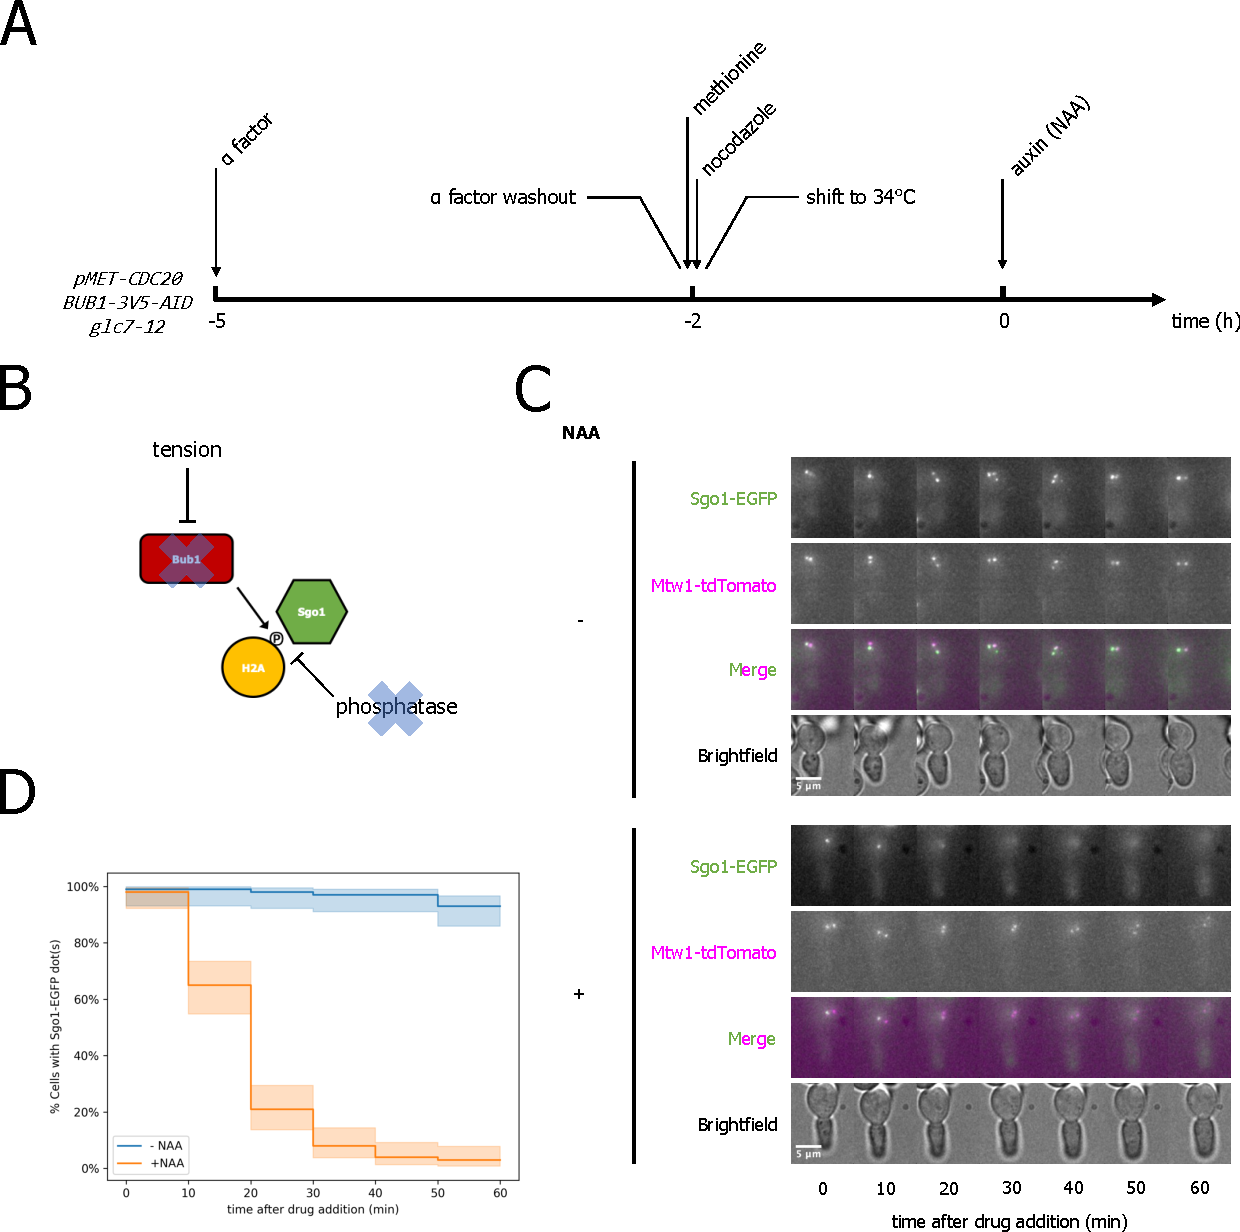
\includegraphics[width=0.9\textwidth]{chapter3/figures/Bub1-AID glc7-12.pdf}
  \caption[PP1 inactivation does not rescue the prompt de-localisation of Sgo1 upon Bub1 depletion in the absence of tension.]{PP1 inactivation does not rescue the prompt de-localisation of Sgo1 upon Bub1 depletion in the absence of tension. (A) Schematics of experimental procedures. (B) Schematics of experimental concept. (C) Montages of representative time-lapse imaging. (D) Survival analysis of the duration of focused Sgo1-EGFP signal. N=30 cells for each strain were followed over time and quantified for the duration of the Sgo1-EGFP signal being focused. Solid lines are Kaplan-Meier survival estimates. The shaded area in the same colour is the 95\% confidence limit of the estimate.}
  \label{fig:bub1aidglc712}
\end{figure}

\subsection{PP1 is required for Bub1 re-localization}

 It has been reported in budding yeast that PP1 could de-phosphorylate the MELT motifs of Spc105, the ortholog of human KNL1, which are important for Bub1 kinetochore localisation \citep{London2012, Roy2019}. We reasoned that the observation that Sgo1 cannot be de-localised upon PP1 inactivation could be due to the retention of Bub1 at the kinetochore in the same condition. To verify this idea, I wanted to study the localisation of Bub1 when PP1 is inactivated. A synchronised G1 to metaphase live-cell imaging at the restrictive temperature of \textit{glc7-12} was performed (Figure~\ref{fig:bub1glc712}A). In wild type, the dynamics of kinetochore-localised Bub1-mNG was as previously described, which was largely reduced at 75 \si{\minute} after G1 release, corresponding to the separation of Mtw1-tdTomato foci. As expected, the drop was not observed in \textit{glc7-12} (Figure~\ref{fig:bub1glc712}B and C), indicating Bub1 de-localisation from the kinetochore upon tension is impaired when PP1 is inactivated. Consistent with the previous experiment, the stabilised inter-kinetochore distance in \textit{glc7-12} was about 0.5 \si{\micro\metre}. Western blotting indicated reduced Bub1 expression in \textit{glc7-12} compared to wild type, probably due to cell death and poorer cell cycle synchronisation. However, it still ruled out the possibility that the increased kinetochore Bub1-mNG fluorescence intensity was because of elevated Bub1 protein level in \textit{glc7-12}. Therefore, combined with the result in the previous section, I concluded that PP1 is required for Sgo1 re-localization due to its role in de-localising Bub1 from the kinetochore. 

\begin{figure}[htbp]
  \centering
  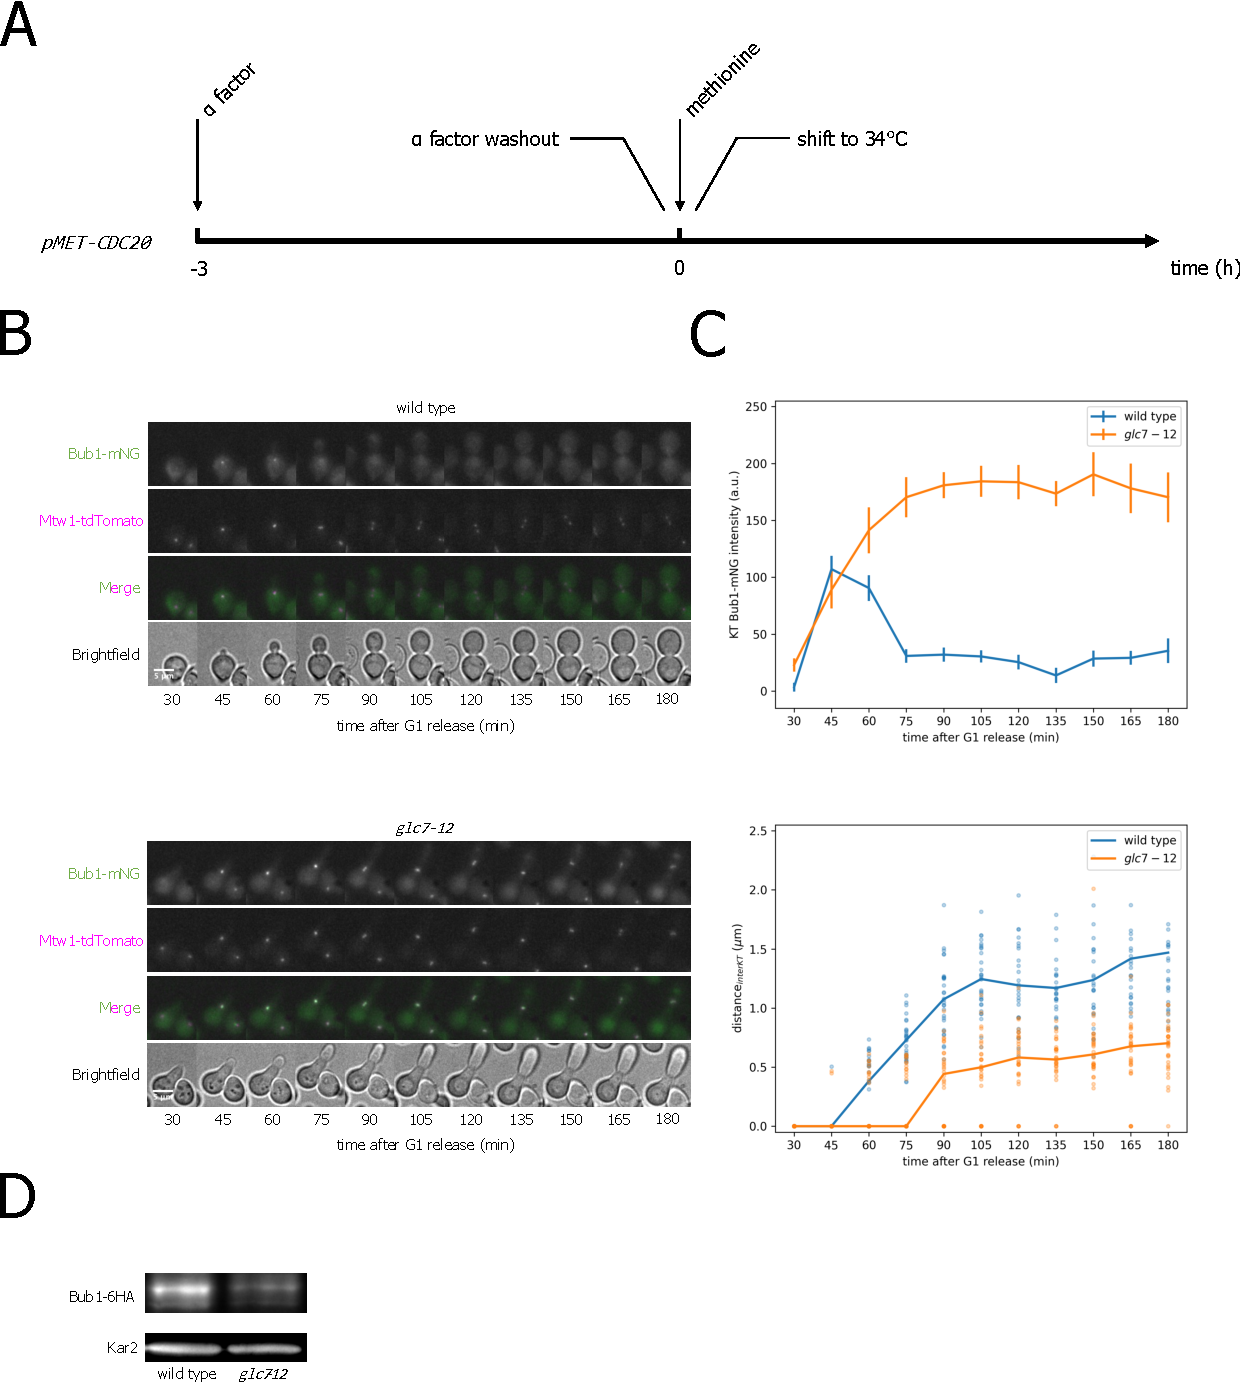
\includegraphics[width=0.9\textwidth]{chapter3/figures/Bub1 glc7-12.pdf}
  \caption[Kinetochore-localised Bub1 is maintained upon PP1 inactivation]{Kinetochore-localised Bub1 is maintained upon PP1 inactivation. (A) Schematics of experimental procedures. (B) Montages of representative time-lapse imaging. (C) N=30 cells for each strain were followed over time and quantified for kinetochore Bub1-mNG fluorescence intensity and inter-kinetochore distance. Top panel: mean fluorescence intensity of Bub1-mNG at the kinetochore as a function of time. The error bar represents the standard error. Bottom panel: Median inter-kinetochore distance as a function of time. Individual data points are shown as dots. (D) Western blotting on cells arrested in metaphase without tension using anti-HA antibody to detect the expression level of Bub1-6HA. Kar2 was used as the loading control.}
  \label{fig:bub1glc712}
\end{figure}

\subsection{Putative PP1 binding motifs of Sgo1 are not required for Sgo1 re-localization}

Interestingly, the budding yeast Sgo1 protein sequence contains the consensus PP1 recognition motif RxVxF and the assisting motif SILK, making it a possible regulatory subunit of PP1 (Figure~\ref{fig:sgo1phosphomutant}A). Given the necessity of PP1 in re-localising Sgo1, we hypothesised that the putative interaction between Sgo1 and PP1 could be the key. To test it, we mutated each or both of the motifs and conducted our standard synchronised G1 to metaphase live-cell imaging (Figure~\ref{fig:sgo1phosphomutant}B). Unexpectedly, in all three mutants, the time Sgo1-EGFP spent as foci were not significantly different from wild type (Figure~\ref{fig:sgo1phosphomutant}C), suggesting these motifs are not required for Sgo1 re-localisation. I further tested the functionality of Sgo1 in the mutants by measuring their benomyl sensitivity. In budding yeast, abnormality in SAC or chromosome segregation does not lead to severe growth defects in an undisturbed cell cycle. However, when challenged by the microtubule de-polymerising drug benomyl, it dramatically reduces the viability. As shown in Figure~\ref{fig:sgo1phosphomutant}D, the negative control \textit{sgo1$\Delta$} showed increased sensitivity to benomyl compared to wild type, representing the loss of Sgo1 functions in mitotic chromosome segregation. On the contrary, the mutants did not show an observable reduction in viability in the presence of benomyl, suggesting Sgo1 functions are intact in those strains. Due to the fact that all the mutants' Sgo1 was tagged by EGFP, I added an additional control \textit{SGO1-EGFP} to test if tagging EGFP itself can cause any change in Sgo1 functions. The similar sensitivity to benomyl between \textit{SGO1-EGFP} and wild type suggested a negative answer to the question. Therefore, I concluded that neither timely re-localisation nor the function of Sgo1 requires its putative PP1 binding sites. 

\begin{figure}[htbp]
  \centering
  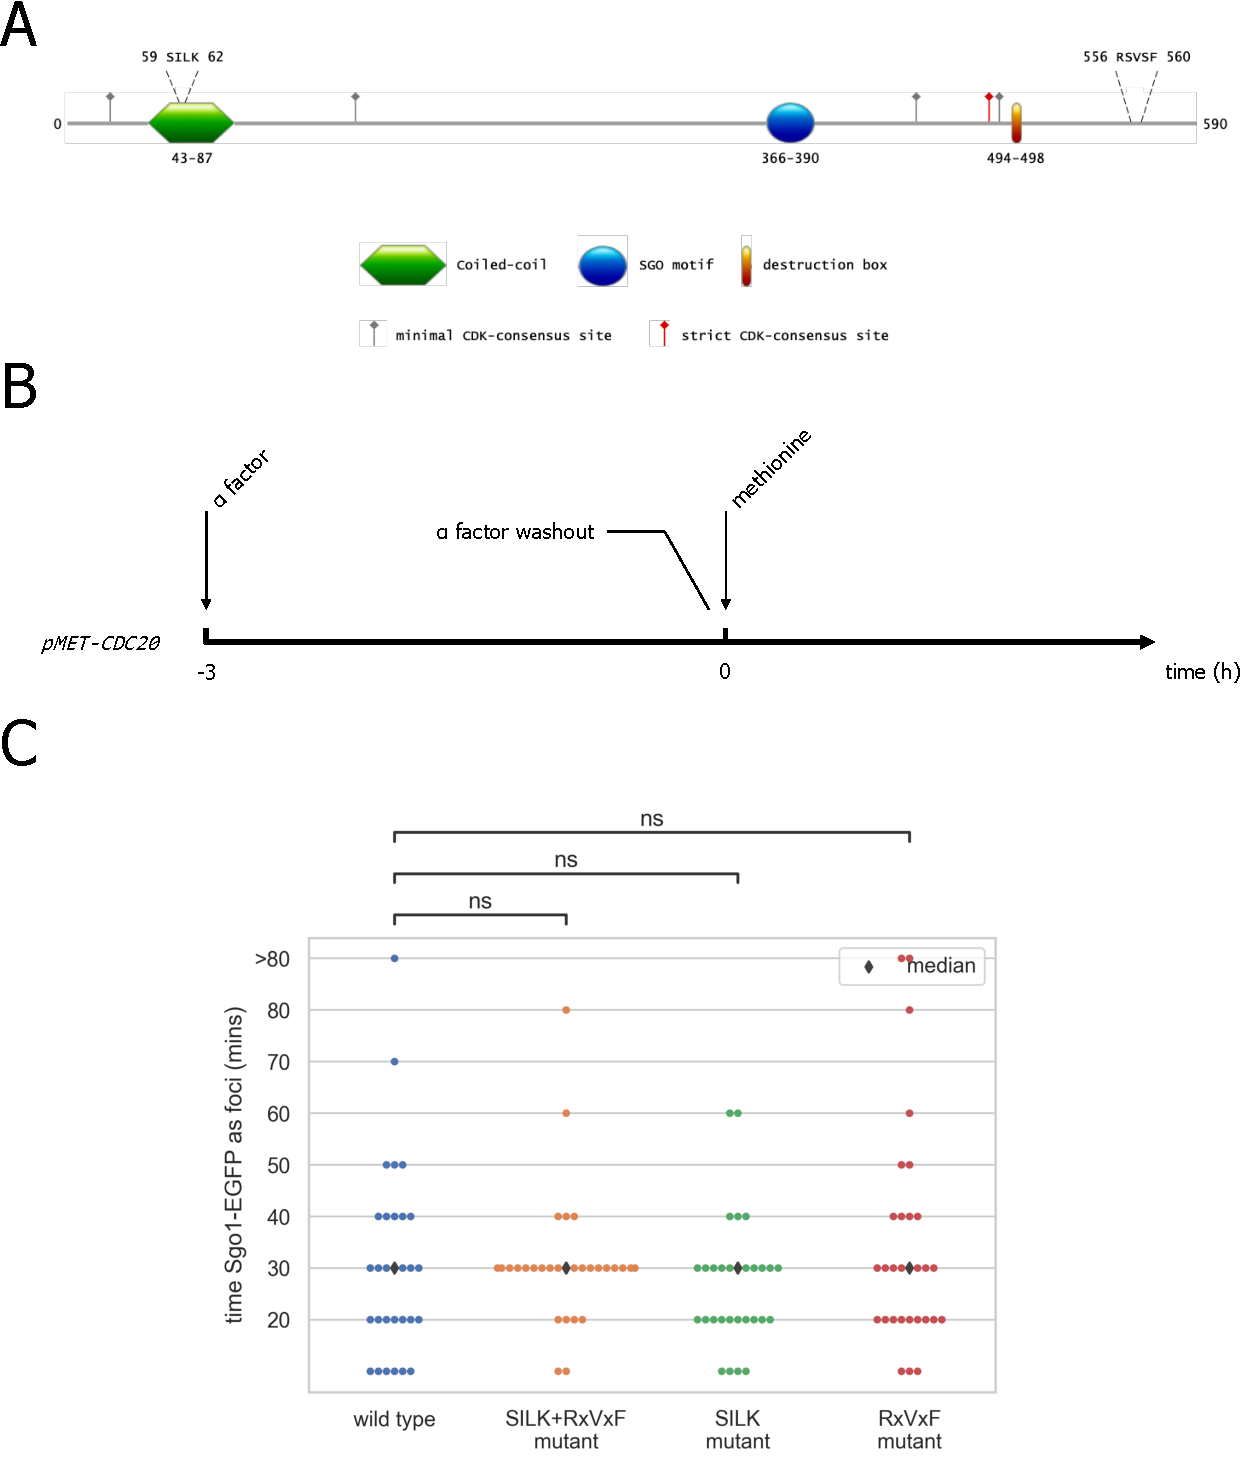
\includegraphics[width=0.9\textwidth]{chapter3/figures/Sgo1 putative PP1 binding mutants.pdf}
  \caption[Neither timely re-localisation nor the function of Sgo1 requires its putative PP1 binding sites]{Neither timely re-localisation nor the function of Sgo1 requires its putative PP1 binding sites. (A) Linear schematics of budding yeast Sgo1 protein. Putative PP1 binding motifs SILK and RSVSF are located at amino acid positions 59-62 and 556-560, respectively. (B) Schematics of the imaging experiment. (C) Quantification of the time of Sgo1-EGFP signal being visualised as foci. The two-tailed independent t-test was used to calculate statistical significance. (*) P<0.05; (ns) not significant. (D) Spot assay testing the benomyl sensitivity of the strains. Five-fold serial dilutions of indicated strains spotted on rich medium with 0 or 10 \si{\micro\gram/\milli\litre} benomyl.}
  \label{fig:sgo1phosphomutant}
\end{figure}

\subsection{PP2A-Rts1 might regulate Sgo1 phosphorylation}

Another attempt to identify the phosphatase involved in the re-localisation of Sgo1 focused on its interacting phosphatase PP2A-Rts1. \cite{Nerusheva2014} showed by ChIP-qPCR that deleting \textit{RTS1} or abolishing Sgo1-PP2A interaction led to an increased association of Sgo1 with the peri-centromeric chromatin in the absence of tension but not upon tension, leaving PP2A as an interesting candidate phosphatase for Sgo1 de-localisation remain to be elucidated. 

PP2A belongs to the type 2 protein phosphatase, PP2, the other phospho-protein phosphatase regulating cellular metabolism than PP1 \citep{Ingebritsen1983ProteinRegulation}. Highly conserved across species, it is demonstrated important in a large number of cellular processes including cell cycle regulation \citep{Janssens2001ProteinSignalling}. Interestingly, despite being one of the most abundant proteins in a cell, accounting for 1\% of total cellular proteins in some cases, PP2A possesses excellent substrate specificity and fine-tuned spatiotemporal regulation \citep{Shi2009Serine/threonineStructure}. This is because of its complicated regulatory mechanism. PP2A core enzyme is composed of a scaffold subunit (A subunit) and a catalytic subunit (C subunit). The core enzyme can interact with one of the various regulatory subunits (B subunit), which targets the substrates specifically, to form the holoenzyme. Four families of regulatory subunit have been identified, namely B (B55), B' (B56), B'' and B''', with each one further having several isoforms \citep{Shi2009Serine/threonineStructure}. In budding yeast, the picture is less complex. There are only two regulatory subunits, Cdc55 and Rts1, corresponding to B and B', respectively \citep{Zhao1997SaccharomycesFunctions}. 

Consistent with PP2A's delicate regulation mechanism, shugoshins specifically interact with the PP2A-B' holoenzyme \citep{Kitajima2006a, Riedel2006, Tang2006a}. Structural data suggest that two human Sgo1 proteins form a dimmer and bind the B' and C subunit of one PP2A holoenzyme through the conserved coiled-coil domain \citep{Xu2009StructureInteraction}. Mutations of the expected contact residues in budding yeast are sufficient to abolish its Sgo1-PP2A interaction, suggesting that this structure is likely to be conserved (Figure~\ref{fig:sgo1phosphorts1d}A). A recent study indicated the existence of further interacting site(s) on Sgo1 with the conserved binding pocket of PP2A-B' \citep{Ueki2021AMitosis}. 

PP2A-B' acts as the effector of many of the shugoshins' functions. It is well established that this interaction is essential for cohesion protection in meiosis I through localised de-phosphorylation of the meiosis-specific kleisin subunit, Rec8, of cohesin \citep{Marston2004a, Kitajima2004a, Katis2004, Rabitsch2004TwoII, Rattani2013Sgol2Oocytes, Llano2008Shugoshin-2Mice, Lee2008} and vertebrate mitosis by counteracting the prophase pathway \citep{Shintomi2009ReleasingSgo1, Rivera2009ShugoshinExtracts, Orth2011ShugoshinMad2, Huang2007, Tang2006a, Tanno2010, McGuinness2005ShugoshinCells, Kitajima2005, Salic2004VertebrateMitosis}. Although there exists conflicting data \citep{Verzijlbergen2014, Eshleman2014}, the bi-orientation promoting function of shugoshins has been reported to require interaction with PP2A-B'\citep{Peplowska2014, Rivera2012}. The interaction has also been indicated involved in spindle checkpoint silencing \citep{Rattani2013Sgol2Oocytes}. 

The commitment to investigating PP2A-Rts1 was decided before the re-establishment of the importance of H2A-pS121 in Sgo1 tension-dependent re-localisation. Instead, we were interested in the hypothesis that Sgo1 post-translational modifications could be the key to its localisation and that PP2A-Rts1 might regulate them. It is derived from the fact that shugoshin phosphorylation has been reported in multiple species \citep{Llano2008Shugoshin-2Mice, Tanno2010, Rattani2013Sgol2Oocytes, Pouwels2007ShugoshinPlk1, Kawashima2007, Lee2014RegulationPhosphorylation, Liu2013, Liu2013a, Clarke2005, Resnick2006INCENPDrosophila, Nogueira2014, Yahya2020} with a few cases affecting its localisation. In humans, CDK phosphorylates Sgo1 at T346 and enables the interaction with cohesin, targeting Sgo1 to the inner centromere. Tension-dependent dephosphorylation of this site then abolishes the interaction and liberates Sgo1 for the association with kinetochore-proximal H2A-pT120, leading to its re-localisation \citep{Liu2013, Liu2013a}. There are also studies reporting CPC-dependent phosphorylation of human Sgo1 affects its localisation \citep{Pouwels2007ShugoshinPlk1, Lee2014RegulationPhosphorylation}. The localisation of \textit{Drosophila} shugoshin ortholog MEI-S332 seems to be dominantly under phospho-regulation. Its centromeric localisation in both mitosis and meiosis requires the phosphorylation by CPC \citep{Resnick2006INCENPDrosophila, Nogueira2014}, whereas the removal during the metaphase-anaphase transition depends on the direct binding and phosphorylation by POLO kinase \citep{Clarke2005}. Despite that the functions have not been elucidated, Sgo1 has been shown to be phosphorylated in budding yeast \citep{Yahya2020, Barton2019MechanismsCerevisiae}. 

To test the hypothesis, we started by asking whether the phosphorylation status of Sgo1 is altered upon \textit{RTS1} deletion. Sgo1-6HIS-3FLAG was immuno-precipitated from wild type or \textit{rts1$\Delta$}. Due to the Sgo1 expression level being cell-cycle-dependent, cells were arrested in metaphase without tension using benomyl for a higher yield. Immuno-precipitated peptides were then digested by trypsin, subjected to phospho-enrichment and identified by MS (Figure~\ref{fig:sgo1phosphorts1d}). Similar to the previous Sgo1 IP-MS done in the lab, amino acid 185-276 could not be revealed in the output data \citep{Barton2019MechanismsCerevisiae}. This is because this region lacks trypsin recognition residue lysine and hence cannot be digested to lengths short enough for MS analysis. Within the two repeats conducted, peptides of amino acid 143-155, 418-433, 475-485 and 484-494 were consistently detected to be phosphorylated. Relative intensities of phosphorylated peptides between wild type and \textit{rts1$\Delta$} were compared (Figure~\ref{fig:sgo1phosphorts1d}C). Phosphorylated peptides showing the same direction of enrichment in both repeats were considered genuine. The analysis indicated that the Sgo1 peptide of amino acid 418-433 showed increased phosphorylation while the peptide of amino acid 484-494 showed reduced phosphorylation in \textit{rts1$\Delta$}. Due to the fact that mass spectrometers can only detect the number of phosphorylation sites in a peptide but not the exact location, all phosphorylatable residues, serine, threonine and tyrosine, in the identified peptide have the potential to be regulated. Therefore, I concluded that PP2A-Rts1 could down-regulate the phosphorylation of Sgo1 at S421, S423 and S426 whereas up-regulate that at S486, S487, T493 and S496. 

\begin{figure}[htbp]
  \centering
  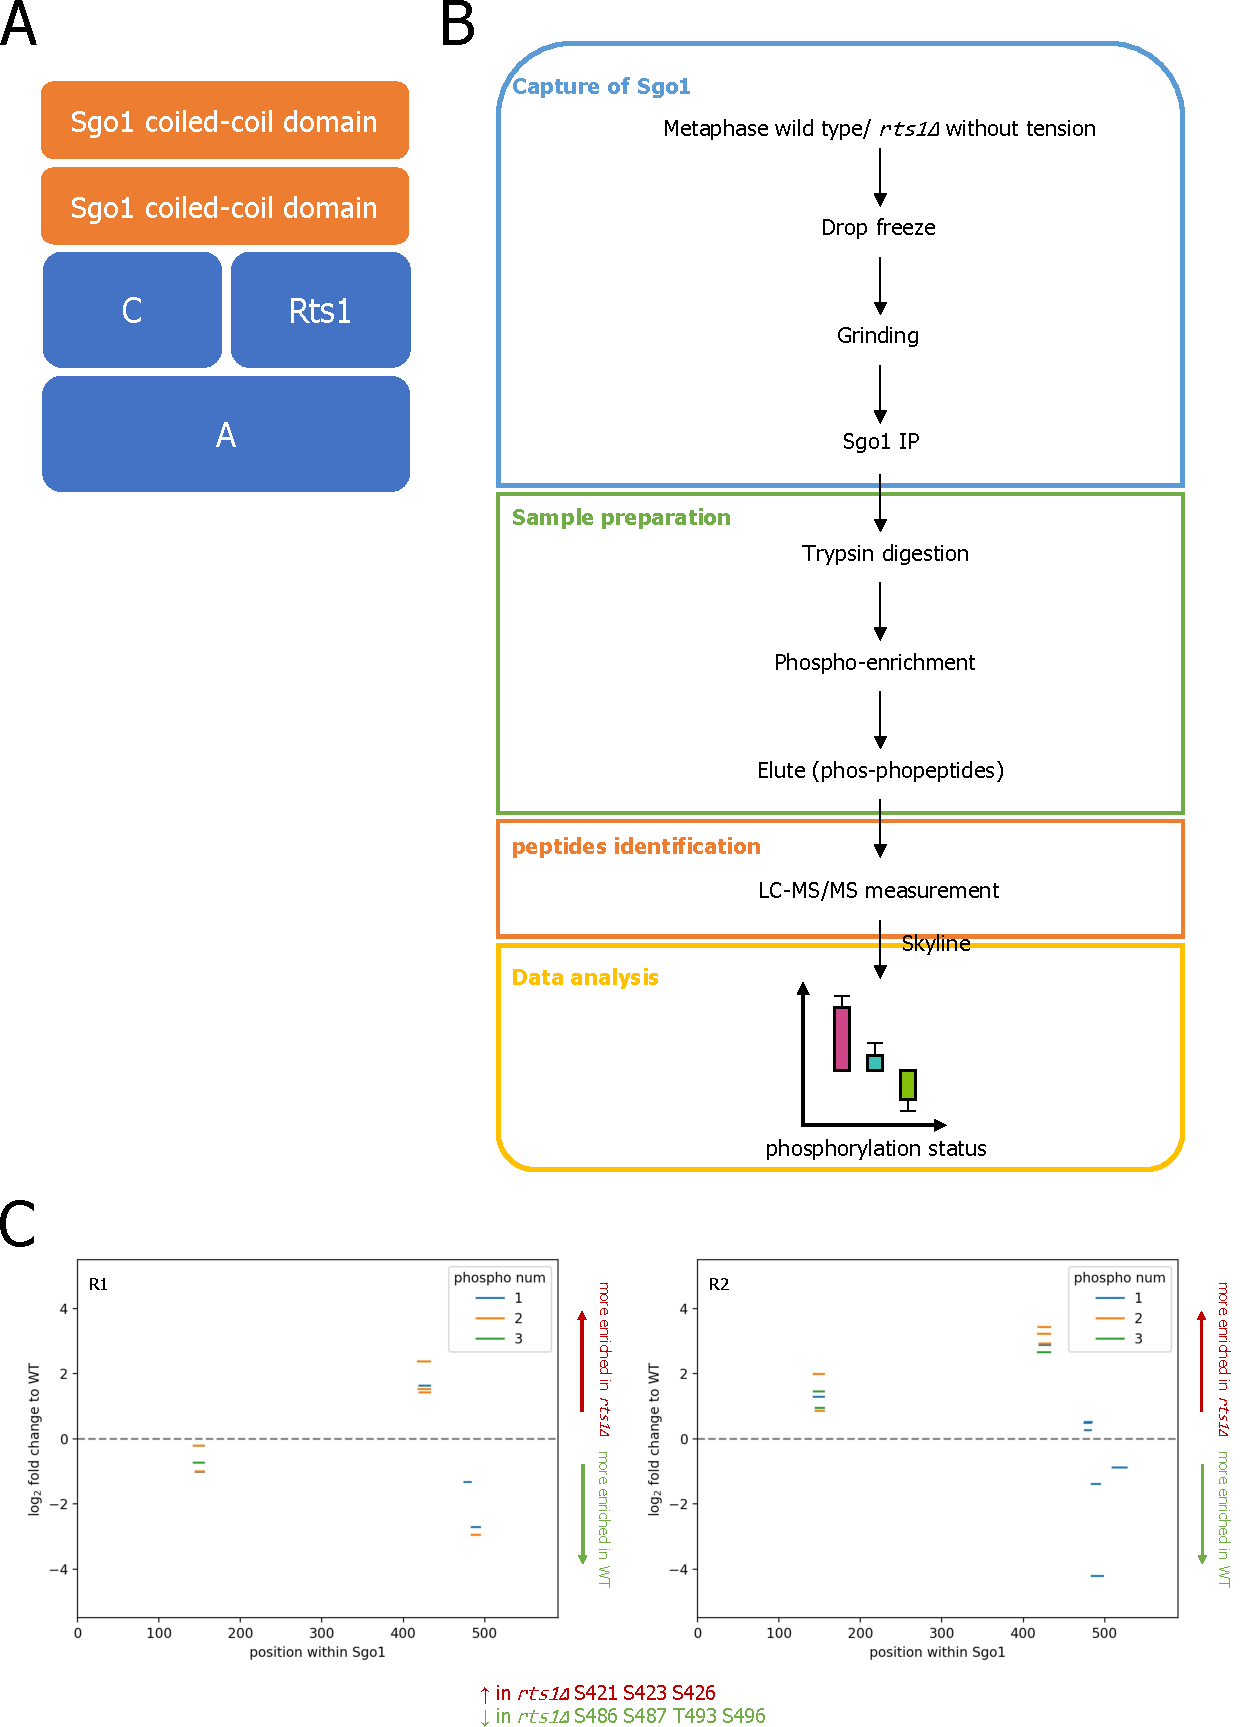
\includegraphics[width=0.9\textwidth]{chapter3/figures/Sgo1 phospho in rts1d.pdf}
  \caption[IP-MS detected changes in Sgo1 phosphorylation in the absence of Rts1]{IP-MS detected changes in Sgo1 phosphorylation in the absence of Rts1. (A) Cartoon of Sgo1-PP2A interaction (revised from \cite{Xu2009StructureInteraction}). (B) Schematics of the Sgo1 IP-MS experiment (C) relative intensities of phosphorylated Sgo1 peptides between wild type and \textit{rts1$\Delta$}. Each bar indicates a single Sgo1 peptide with amino acids of Sgo1 indicated on the x-axis. mono-, di- and tri-phosphorylated forms of the same peptide are indicated by differently coloured bars. Amino acid residues potentially more phosphorylated in \textit{rts1$\Delta$} are marked in red and those potentially less phosphorylated are marked in green. }
  \label{fig:sgo1phosphorts1d}
\end{figure}

\nomenclature{IP}{ImmunoPrecipitation}

\subsection{Sgo1 re-localization is independent of the phosphorylation at S421 or S487}

To test the functional relevance of the potential Sgo1 phosphorylation regulated by PP2A-Rts1, I wanted to measure the benomyl sensitivity of Sgo1 phospho-mutants to assess the functionality of their Sgo1 proteins. Therefore, I picked one site from each group identified as down-regulated or up-regulated by PP2A-Rts1 in the previous experiment and acquired both the phospho-null and phospho-mimic mutants from the Marston lab yeast collections. Wild type and \textit{sgo1$\Delta$} were included as the positive and negative control. The result of the spot assay was shown in Figure~\ref{fig:sgo1phosphomutants}A. \textit{sgo1$\Delta$} indicated strong sensitivity to benomyl as expected. Interestingly, the phospho-null mutant of the down-regulated site (S421A) and the phospho-mimic mutant of the up-regulated site (S487D) showed mildly increased viability compared to wild type on the benomyl-containing plate whereas their opposite phospho-mutants (S421D and S487A) had slightly reduced viability. This suggests that Sgo1 phosphorylation regulated by PP2A-Rts1 is relevant to its mitotic functions. However, \textit{rts1$\Delta$} also showed comparable benomyl sensitivity to the wild type, arguing against the idea. 

Since the aim of the project is to understand the mechanism of Sgo1 localisation regulation, I decided to leave the confusion aside and directly investigated the localisation of Sgo1 in those mutants. Hence, I used live-cell imaging to determine the duration of Sgo1 staying at the peri-centromere as in the previous experiments (Figure~\ref{fig:sgo1phosphomutants}B). As measured before, the duration of Sgo1-EGFP being as foci had a median of 30 \si{\minute}. The phospho-mutants were not statistically different from the wild type, suggesting that, whether genuinely phosphorylated or not, these sites are not involved in regulating Sgo1 localisation. Thus, I concluded that Sgo1 re-localization is independent of the phosphorylation at S421 or S487 (Figure~\ref{fig:sgo1phosphomutants}C). 

\begin{figure}[htbp]
  \centering
  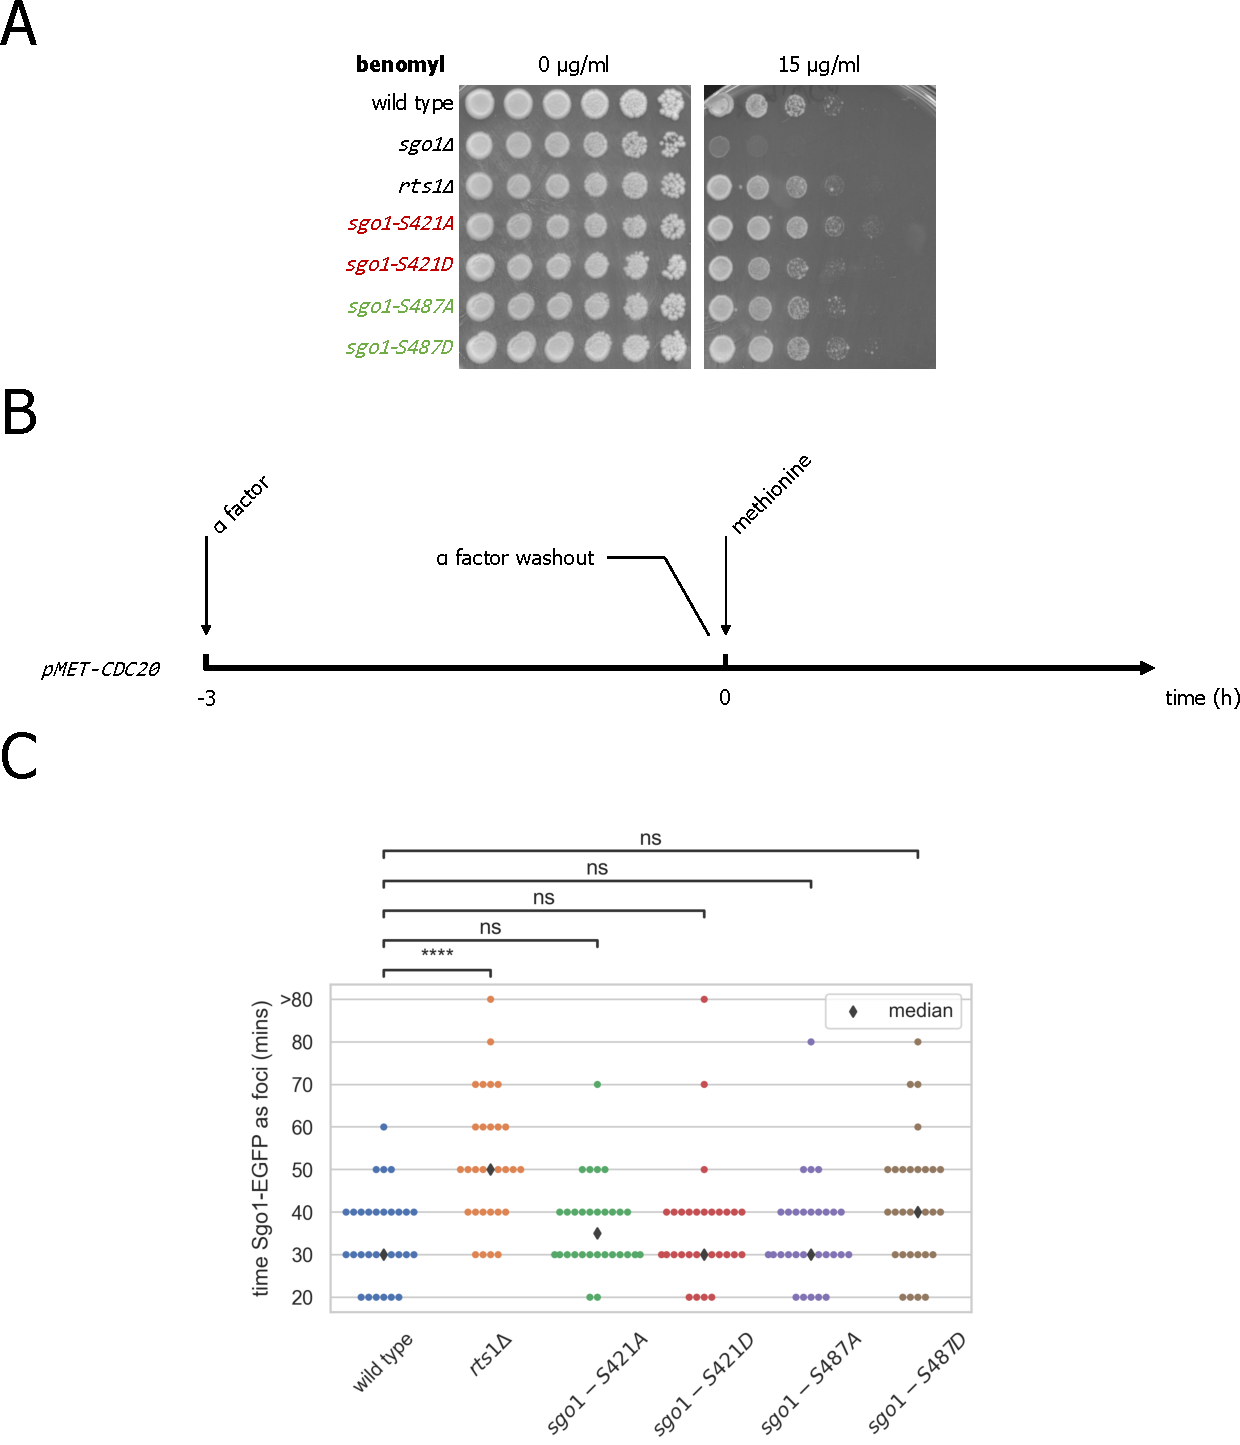
\includegraphics[width=0.9\textwidth]{chapter3/figures/sgo1 phospho mutants.pdf}
  \caption[Phenotypical characterisation of mutants with putative PP2A-Rts1-regulated phosphorylation sites of Sgo1 mutated]{Phenotypical characterisation of mutants with putative PP2A-Rts1-regulated phosphorylation sites of Sgo1 mutated. (A) Spot assay testing the benomyl sensitivity of the strains. Five-fold serial dilutions of indicated strains spotted on rich medium with 0 or 15 \si{\micro\gram/\milli\litre} benomyl. The red and green colours indicate whether the site is potentially more or less phosphorylated in \textit{rts1$\Delta$}. (B) Schematics of the imaging experiment. (C) Quantification of the time of Sgo1-EGFP signal being visualised as foci. The two-tailed independent t-test was used to calculate statistical significance. (****) P<0.0001; (ns) not significant. }
  \label{fig:sgo1phosphomutants}
\end{figure}

\subsection{PP2A-Rts1 is required for timely sister kinetochore separation}

On the contrary to the phospho-mutants, \textit{rts1$\Delta$} did show a 20-\si{\minute} increase in the time Sgo1-EGFP being visualised as foci in Figure~\ref{fig:sgo1phosphomutants}C, which is in consistency with \cite{Nerusheva2014}. This suggests PP2A-Rts1 is required for the timely removal of Sgo1 from the peri-centromere. However, the lack of information on inter-kinetochore distance in that experiment prevented us from distinguishing between (A) PP2A-Rts1 is the phosphatase de-localising Sgo1, likely by de-phosphorylating H2A-pS121, and (B) PP2A-Rts1 is required to generate enough tension for Sgo1 re-localisation on time. Therefore, I decided to include the inter-kinetochore distance measure in the experiment. Besides, The PP2A-binding-defective mutant \textit{sgo1-3A} was also included to study if the interaction is important here. The standard G1-to-metaphase live-cell imaging was conducted as previously described (Figure~\ref{fig:sgo1rts1mutants}A). Notably, by the time I performed the experiment, the camera of our wide-field microscope was swapped to Photometrics Prime 95B due to a product demonstration, resulting in a different-sized field of view from the previous experiments (Figure~\ref{fig:sgo1rts1mutants}B). In spite of that, the dynamics of Sgo1-EGFP localisation and inter-kinetochore distance of the wild type are the same as before. The result indicated that, despite a 15-\si{\minute} delay in the emergence, the vanish of Sgo1-EGFP foci was around 30 \si{\minute} later in \textit{rts1$\Delta$} (Figure~\ref{fig:sgo1rts1mutants}C). This leads to a 15-\si{\minute} increase in the duration of Sgo1 staying as foci, which is comparable to the results in Figure~\ref{fig:sgo1phosphomutants}C and \cite{Nerusheva2014}. However, when examining the inter-kinetochore distance, \textit{rts1$\Delta$} showed about 30 \si{\minute} delay than the wild type (Figure~\ref{fig:sgo1rts1mutants}C), indicating that PP2A-Rts1 is also required for timely separation of sister kinetochores. This means that the delay in Sgo1 de-localisation in \textit{rts1$\Delta$} is likely due to its delayed tension establishment, arguing against the hypothesis that PP2A-Rts1 is the phosphatase directly removes Sgo1. It can also be supported by the observation that the inter-kinetochore distance for Sgo1 to disperse was roughly the same between \textit{rts1$\Delta$} and the wild type. In further support, \textit{sgo1-3A}, whose Rts1 centromeric enrichment is abolished in mitosis \citep{Eshleman2014}, showed a very similar Sgo1-EGFP and Mtw1-tdTomato dynamics to the wild type (Figure~\ref{fig:sgo1rts1mutants}C). 

As mentioned before, Sgo1 association with the peri-centromere chromatin was increased in \textit{rts1$\Delta$} in the absence of tension. Apart from its original aim, this imaging experiment also provided an opportunity to alternatively test the finding. Hence, I quantified the fluorescence intensities of Sgo1-EGFP foci for the wild type and \textit{rts1$\Delta$} while tension was not established. Surprisingly, there was no significant difference observed (Figure~\ref{fig:sgo1rts1mutants}D). One possible explanation is that, albeit the total amount remains similar, the turnover rate of peri-centromeric Sgo1 might be reduced in \textit{rts1$\Delta$}, resulting in increased ChIP signal. 

\begin{figure}[htbp]
  \centering
  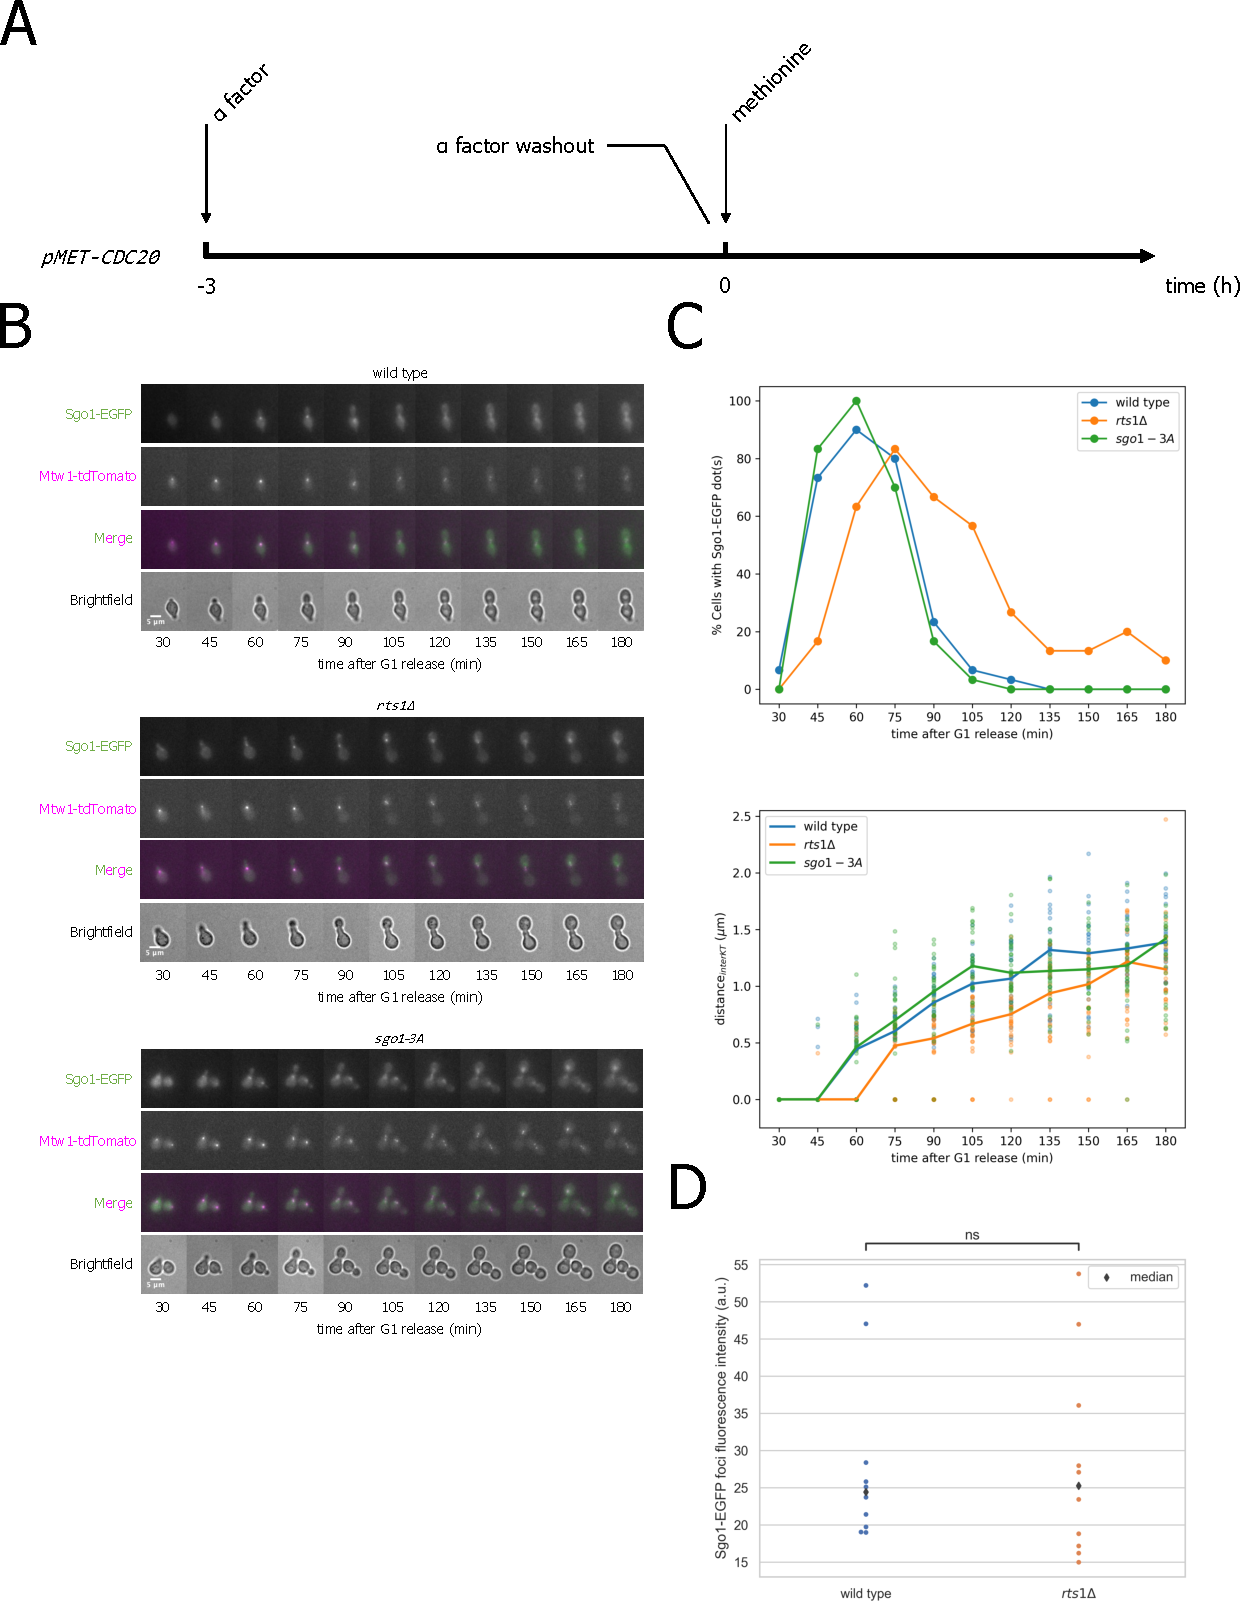
\includegraphics[width=0.9\textwidth]{chapter3/figures/Sgo1 rts1 mutants.pdf}
  \caption[PP2A-Rts1 is required for timely sister kinetochore separation but not for reducing Sgo1 level at peri-centromere]{PP2A-Rts1 is required for timely sister kinetochore separation but not for reducing Sgo1 level at peri-centromere. (A) Schematics of the imaging experiment. (B) Montages of representative time-lapse imaging. (C) N=30 cells for each strain were followed over time and quantified. Top panel: the percentage of cells with Sgo1-EGFP foci was shown as a function of time. Bottom panel: median inter-kinetochore distance as a function of time. Individual data points are shown as dots. (D) N=10 cells for the wild type and \textit{rts1$\Delta$} were quantified for the highest fluorescence intensities of Sgo1-EGFP foci among all frames. (ns) not significant.}
  \label{fig:sgo1rts1mutants}
\end{figure}

\subsection{Tension induces mild chromosome condensation}

Interphase chromosomes have to be condensed during mitosis to reduce space occupied, remove sister chromatids catenation, provide physical properties able to withstand forces during movement and therefore facilitate faithful chromosome segregation \citep{Antonin2016ChromosomeMitosis, Piskadlo2016NovelCondensation, Beseda2020MitoticVariability, Takahashi2019FoldingChromosomes}. The current model of chromosome condensation recognises it to be driven by the condensin-mediated compaction pathway and histone-mediated contraction pathway in parallel \citep{Wilkins2014, Kruitwagen2015}. Interestingly, key players from both pathways have been reported to interact with shugoshin or the H2A phosphorylation enabling Sgo1 chromatin association, including Topoisomerase II \citep{Zhang2020FunctioningMitosis} and condensin itself \citep{Verzijlbergen2014, Yahya2020} from the condensin-mediated pathway and CPC \citep{Abad2022MechanisticCPC} from the histone-mediated pathway. This makes Sgo1 and H2A phosphorylation potentially important in chromosome condensation. Indeed, in budding yeast, both compaction and contraction were impaired in the absence of Sgo1 \citep{Kruitwagen2018}. 

Our previous finding that H2A-pS121 and possibly Sgo1 re-distribute from the centromere to the whole genome by tension provides a potential molecular explanation for the model proposed by \cite{Kruitwagen2018}, where SAC silencing is required for further chromosome condensation. If it is true, we would expect increased chromosome condensation upon the establishment of tension. Hi-C has been used to investigate chromosome condensation in various species \citep{Kakui2017Condensin-mediatedYeast, Schalbetter2017SMCContext, Lazar-Stefanita2017CohesinsCellcycle, Naumova2013OrganizationChromosome}. To test the hypothesis, I took advantage of Hi-C experiments conducted by \cite{Paldi2020ConvergentPericentromeres} and compared data from metaphase cells with and without tension. The Hi-C ratio map revealed the conformational changes in peri-centromere chromatin by tension, indicated by the red cross around the core centromeres, as reported in the paper (Figure~\ref{fig:Hi-C+-tension}A). Besides, the tension sample showed increased inter-centromere contact (the blue dots at the intersection of centromeres of different chromosomes) and increased inter-arm contact (the blue 'wings' extending diagonally from the centromeres). Importantly, It indicated a mild increase in long-range \textit{in cis} contact (the two light blue lines beside the diagonal) and a mild decrease in short-range contact (the light red line along the diagonal), both of which are the characteristics of chromosome condensation described by \cite{Kakui2018SMCLandscape}. As an alternative to the ratio map, I also visualised the Hi-C difference map, where the contact probability at each coordinate of one sample is simply subtracted by that of the other one (Figure~\ref{fig:Hi-C+-tension}B). Consistently, it also revealed the mild increase in long-range \textit{in cis} contact and the decrease in short-range contact. The Hi-C difference further showed blue dots along the diagonal, which might represent increased loop formation in the tension sample. To obtain a more quantitative view, the contact probabilities of the genome excluding the centromeres were plotted as a function of distance (Figure~\ref{fig:Hi-C+-tension}C). Albeit to a mild extent, the difference between curves of tension and no tension sample did mimic the difference between interphase and mitosis in different species \citep{Kakui2018SMCLandscape}. The contact probabilities of the tension sample showed a reduction in the distances less than 20 kb, an increase in 20 to around 150 kb and another decrease in distances greater, which can also be inferred from the slope plot below. This is in good quantitative agreement with other chromosome condensation research using budding yeast, where the interval of increased contact probability was observed between 10 to 100 kb \citep{Kakui2018SMCLandscape, Schalbetter2017SMCContext, Lazar-Stefanita2017CohesinsCellcycle}. Notably, the increase in long-range interaction was stronger at chromosomal regions further away from the centromeres, a phenomenon that has been reported in budding yeast chromosome condensation \citep{Neurohr2011ALength}. Visualisation of individual chromosomes identified a strong increase in long-range interaction at chrXII, where rDNA was located, further supporting that the difference observed here is due to genuine chromosome condensation rather than artefacts from data analysis. Therefore, I concluded that a mild chromosome condensation is induced upon the establishment of tension. 

\begin{figure}[htbp]
  \centering
  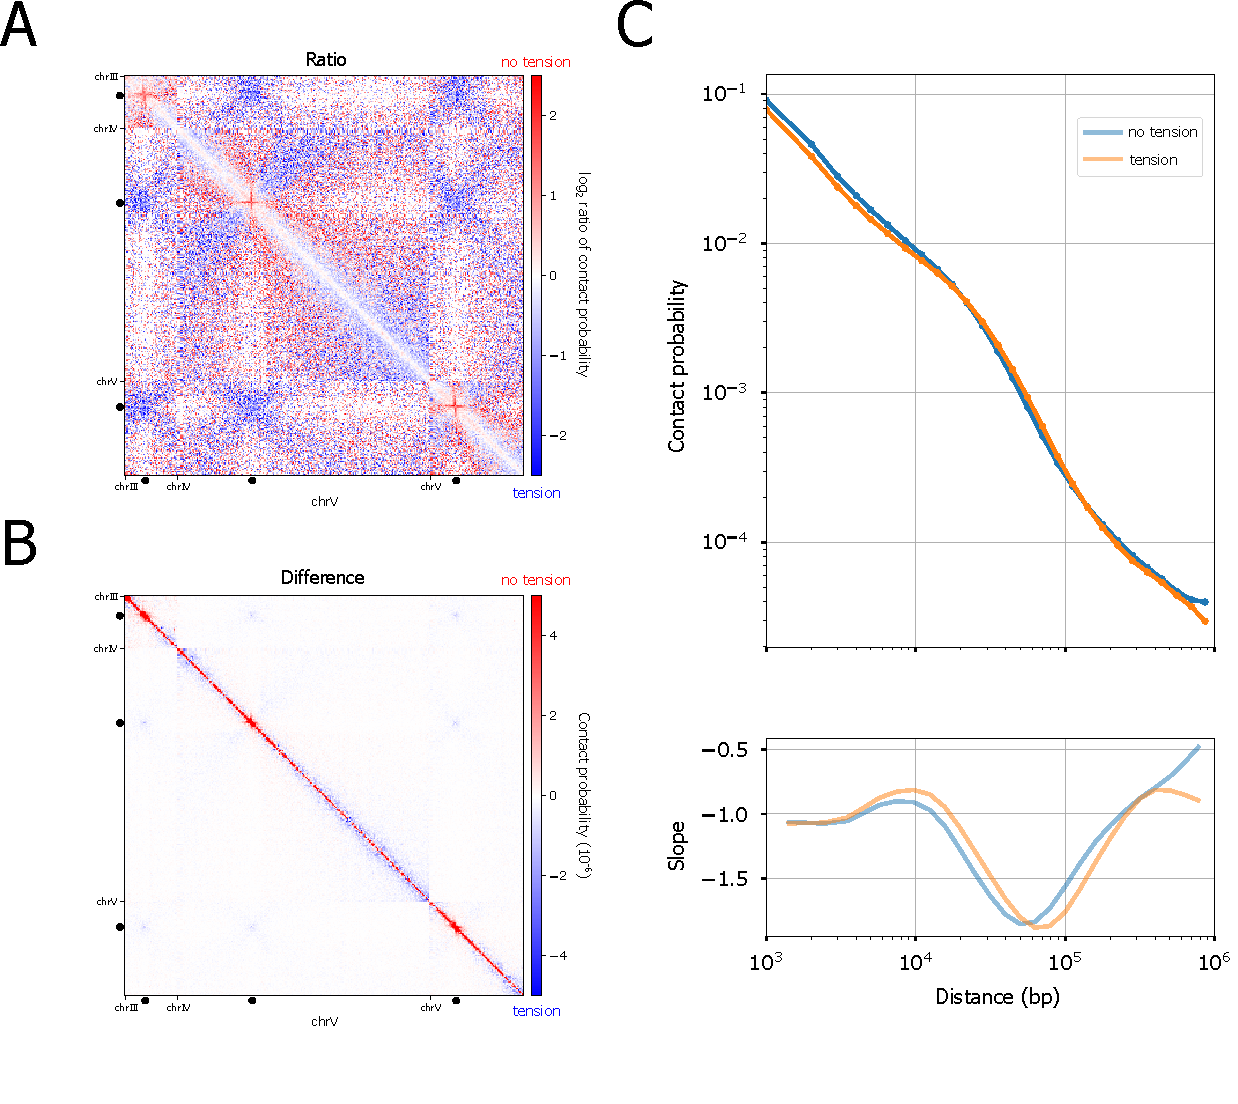
\includegraphics[width=0.9\textwidth]{chapter3/figures/+-tension Hi-C.pdf}
  \caption[Long-range \textit{in cis} interactions are mildly increased upon the establishment of tension]{Long-range \textit{in cis} interactions are mildly increased upon the establishment of tension. (A-C) Analyses of Hi-C of cells arrested in metaphase with or without tension from \cite{Paldi2020ConvergentPericentromeres}. (A) Hi-C ratio map (5kb binning) of chromosome III, IV and V. Black dots represent the coordinates of the core centromeres. (B) Hi-C difference map (5kb binning) of chromosome III, IV and V (no tension - tension). Black dots represent the coordinates of the core centromeres. (C) Top: median contact probability as a function of genomic distance, excluding contacts across the 50kb regions flanking the core centromeres. Bottom: The slopes of the curves above.}
  \label{fig:Hi-C+-tension}
\end{figure}

\subsection{Cohesin is not required for the concentration of Sgo1 at centromere-proximal location}

In the absence of tension, the association of Sgo1 with chromatin shows three major peaks, at the core centromere and the two peri-centromeric borders \citep{Verzijlbergen2014, Paldi2020ConvergentPericentromeres}. Intriguingly, this is different from H2A-pS121, whose distribution profile is rather bell-shaped (Figure~\ref{fig:sgo1comparison}). Given its necessary role in localising Sgo1, this result is quite surprising and it suggests that there might be other factors determining Sgo1 localisation. It has been shown in humans that interaction with cohesin is key to Sgo1 localisation to the inner centromere \citep{Liu2013a}. Also, in budding yeast, cohesin depletion results in a reduction in the ChIP signal at the centromeric region \citep{Verzijlbergen2014}. These results supported the idea that cohesin could be the factor mentioned above. However, this is in contradiction with the experiment used to demonstrate shugoshin's function in tension sensing, where Sgo1 is shown to be required for delaying cell cycle progression upon cohesin depletion \citep{Indjeian2005a}. As kinetochore-microtubule attachment is undisturbed, this experiment implies that Sgo1 should be localised at the peri-centromere to maintain CPC localisation for error correction. 

\begin{figure}[htbp]
  \centering
  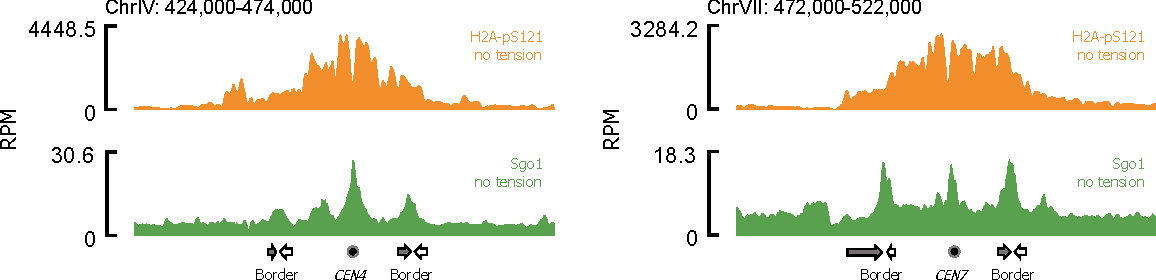
\includegraphics[width=0.9\textwidth]{chapter3/figures/Sgo1 comparison.pdf}
  \caption[H2A-pS121 ChIP-seq profile is qualitatively different from Sgo1]{H2A-pS121 ChIP-seq profile is qualitatively different from Sgo1. ChIP-seq profiles of H2A-pS121 and Sgo1 \citep{Paldi2020ConvergentPericentromeres} at the 50kb regions of chromosome IV and VII centromeres. Convergent genes at the peri-centromere borders are marked as arrows. }
  \label{fig:sgo1comparison}
\end{figure}

To solve the enigma, we sought to investigate the localisation of Sgo1 upon cohesin depletion by microscopy method. Cells used for Sgo1-EGFP imaging that additionally bear \textit{pMET-SCC1} were used and the experimental procedure was the same as the one in Figure~\ref{fig:bub1metscc1} (Figure~\ref{fig:sgo1metscc1}A). Surprisingly, unlike the wild type, Sgo1-EGFP remained its foci signal till the end of the experiment in \textit{pMET-SCC1} (Figure~\ref{fig:sgo1metscc1}B and C). This result is in favour of the classic genetics experiment \citep{Indjeian2005a} but is against the ChIP-qPCR results \citep{Verzijlbergen2014}. It might again reflect the fundamental difference in methodology principles between ChIP and fluorescence microscopy as in Figure~\ref{fig:sgo1rts1mutants}. Another possible explanation is that cohesin is not required for the recruitment of Sgo1 to the centromeric region but for its subtle localisation to a more confined sub-region as in humans \citep{Liu2013a}. Furthermore, the fact that Sgo1 localisation resembles Bub1 upon cohesin depletion (Figure~\ref{fig:bub1metscc1}) supports the notion from previous experiments that the localisation of Bub1 and H2A-pS121 is the determining factor of Sgo1 localisation. 

To ensure the efficacy of cohesin, I further conducted a mitotic time-course experiment using the \textit{pMET-SCC1} strain in the presence and absence of methionine, followed by western blotting to measure the expression level of Scc1. Spindle IF was used to determine the stages of the cell cycle (Figure~\ref{fig:sgo1metscc1}D). Albeit the sub-optimal synchronisation (Figure~\ref{fig:sgo1metscc1}E), it can still be seen that cells went through metaphase and anaphase in the absence of methionine, whereas they were arrested in metaphase when methionine was added. As expected, without methionine, Scc1 accumulated since the G1 release but started to decrease upon anaphase onset, accompanied by the emergence of the band at lower molecular weight, which represents the cleaved products \citep{Alexandru2001PhosphorylationYeast}. In the presence of methionine, the lack of the band representing cleaved products agreed with the metaphase arrest indicated by the spindle IF (Figure~\ref{fig:sgo1metscc1}E). Importantly, at the same exposure time, the Scc1 signal is largely reduced compared to no Scc1 depletion but still remained visible, suggesting an incomplete depletion (Figure~\ref{fig:sgo1metscc1}D). Therefore, we could not rule out the possibility that residual cohesin is sufficient to support the concentration of Sgo1-EGFP at centromere proximity. 

\begin{figure}[htbp]
  \centering
  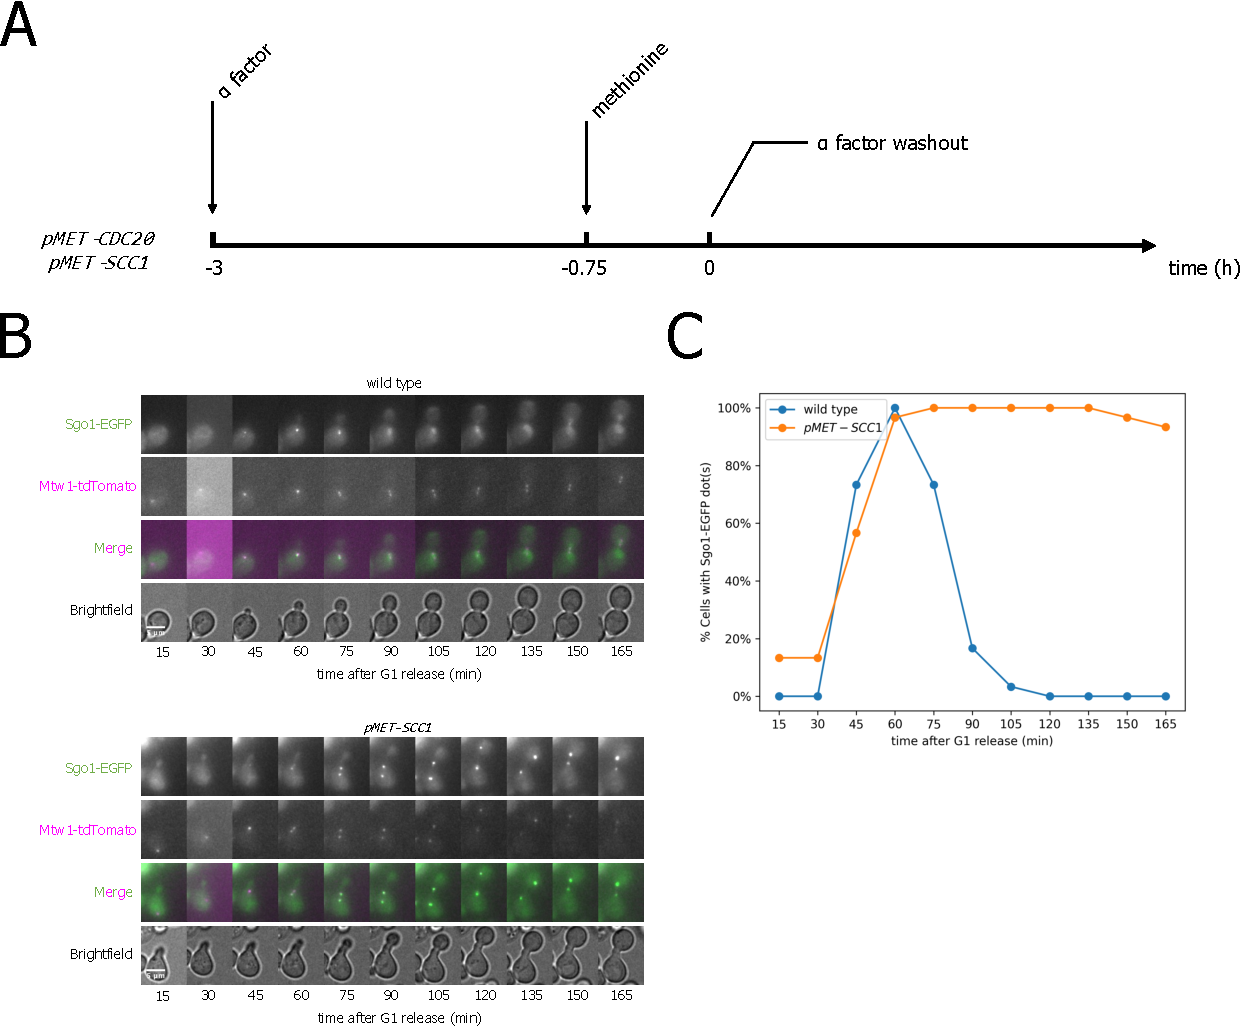
\includegraphics[width=0.9\textwidth]{chapter3/figures/Sgo1 pMET-SCC1.pdf}
  \caption[Sgo1 remains concentrated proximal to the centromere upon cohesin depletion]{Sgo1 remains concentrated proximal to the centromere upon cohesin depletion. (A) Schematics of experimental procedures. (B) Montages of representative time-lapse imaging. (C) N=30 cells for each strain were followed over time and quantified. The percentage of cells with Sgo1-EGFP foci was shown as a function of time. (D) Western blotting on cells arrested in metaphase without tension using anti-myc antibody to detect the expression level of Scc1-myc18. Pgk1 was used as the loading control. (E) The proportion of cells with metaphase or anaphase spindle over time by tubulin IF.}
  \label{fig:sgo1metscc1}
\end{figure}

\nomenclature{qPCR}{quantitative Polymerase Chain Reaction}
\nomenclature{RPM}{Reads Per Million}

\section{Discussion}
\subsection{Model for tension-dependent re-localisation of Sgo1}

Tension-dependent re-localisation of Sgo1 has been observed in various species and shown to be functionally important. To understand the mechanism by which budding yeast Sgo1 is re-localised under tension, we started with a naive model (Figure~\ref{fig:naive}) where the balance between Bub1 and a counteracting phosphatase determines the level of local phosphorylation important for the localisation of Sgo1, and tension is able to reduce the local activity of Bub1 at peri-centromere and hence flip the balance towards the phosphatase. Yet, questions remained to be answered for this model. It was unknown how Bub1 activity in a particular area is regulated by tension. Bub1 substrate H2A-S121 is known to be required for Sgo1 localisation but whether the regulation of its phosphorylation is the key to Sgo1 re-localisation was untested. Lastly, the identity of the phosphatase involved was also to be elucidated. 

The observations that Bub1 remains at the kinetochore after the establishment of tension \citep{Bokros2021YeastAnaphase, Nerusheva2014} and that contacts between the core centromere and the peri-centromere borders are reduced by tension \citep{Paldi2020ConvergentPericentromeres} led us to the hypothesis that tension could regulate local Bub1 activity by pulling kinetochore-localised Bub1 from its substrate(s) at the peri-centromere borders. However, the tetO arrays at one peri-centromere border stayed a similar distance to one of the Bub1-mNG foci regardless of the tension, making it difficult to draw a conclusion on this hypothesis (Figure~\ref{fig:periCEN}). Instead, it was noticed that the fluorescence intensity of Bub1 foci experienced a sharp decrease coinciding with the separation of sister kinetochores, suggesting the kinetochore localisation of Bub1 might be regulated by tension (Figure~\ref{fig:bub1mtw1}). This raised an alternative explanation that tension could de-localise Bub1 from the kinetochore and hence it is physically separated from its peri-centromeric substrate(s). A following experiment revealed that Bub1-mNG foci maintained their intensity when tension is abolished by cohesin depletion, indicating tension is indeed required for Bub1 de-localisation on top of kinetochore-microtubule attachment (Figure~\ref{fig:bub1metscc1}). The sufficiency of Bub1 removal for Sgo1 de-localisation was demonstrated by the prompt dispersal of Sgo1-EGFP foci upon Bub1 depletion (Figure~\ref{fig:bub1aid}). Moreover, with similar cell cycle progression, indicated by the inter-kinetochore distance, cells bearing \textit{Bub1-EGFP} had their fluorescence foci dimmed 15 \si{\minute} earlier than the ones bearing \textit{SGO1-EGFP}, suggesting Bub1 de-localisation happens before Sgo1 de-localisation (Figure~\ref{fig:bub1sgo1}). Though the experiment would be more solid if Bub1 and Sgo1 were tagged with fluorescence proteins of different colours, similar maturation time and sufficient brightness, in a single strain. Nevertheless, the experiments above pointed to the conclusion that the de-localisation of Bub1 from the kinetochore by tension is upstream Sgo1 tension-dependent re-localisation. 

Due to its well-established role in shugoshin localisation in various species and the fact that it is a substrate of Bub1, it is tempting to hypothesise that the phospho-regulation of H2A-S121 is the key to tension-dependent re-localisation of Sgo1. To test this idea, we made phospho-specific antibodies. It was found that this phosphorylation was quickly reduced when Bub1 is depleted, which fits the predicted behaviour of the substrate by the naive model (Figure~\ref{fig:ph2abub1aid}). In further support of the hypothesis, albeit the total H2A-pS121 remained at similar levels in the presence or absence of tension, ChIP-seq revealed distinct distributions over the genome, with the phosphorylation being more spread along the chromosome arms upon tension whereas more enriched at centromeres in the tension-less condition (Figure~\ref{fig:ph2achipseq2nd}). This re-distribution corresponds well with the re-localisation of Sgo1, making H2A-S121 plausible to be the substrate in the naive model. However, the notion is in contradiction with the results by \cite{Nerusheva2014} that Sgo1 can still be localised to the peri-centromere in the H2A phospho-mimic mutant H2A-S121D in a Bub1-dependent manner. It was then noticed a likely strain confusion in those experiments (Figure~\ref{fig:h2as121dseq}). ChIP-qPCR experiment with re-constructed strains showed a low association of Sgo1 with peri-centromeric chromatin in the phospho-mimic mutant, indicating that Sgo1 cannot be concentrated if the H2A phosphorylation is homogeneously distributed over the genome, which emphasised the importance of the spatial regulation of H2A-pS121 to Sgo1 localisation (Figure~\ref{fig:sgo1chiph2amutants}). The conclusion is further confirmed by the results from an imaging experiment, where Sgo1-EGFP did not form any focus in the H2A phospho-mimic mutant (Figure~\ref{fig:sgo1imagingh2amutants}). Therefore, I concluded that the re-distribution of H2A-pS121 is likely to underlie the re-localisation of Sgo1. 

Regarding the phosphatase counteracting Bub1 to de-phosphorylate H2A-pS121, we hypothesised PP1 and PP2A-Rts1 as potential candidates. Interestingly, \textit{GLC7}, the gene encoding the PP1 catalytic subunit, showed genetic interaction with \textit{SGO1}, indicated by that \textit{sgo1$\Delta$} is able to suppress the temperature sensitivity of \textit{glc7-10} and \textit{glc7-12} mutant (Figure~\ref{fig:growthassay}). Microscopy then revealed that Sgo1-EGFP foci did not vanish even though enough tension had been generated in those mutants, showing that PP1 is required for the re-localisation of Sgo1 (Figure~\ref{fig:sgo1glc712} and Figure~\ref{fig:sgo1glc710}). Nevertheless, Bub1 depletion after Sgo1 had been localised still caused quick dispersal of Sgo1-EGFP foci despite PP1 being inactivated, suggesting that the requirement of PP1 for Sgo1 de-localisation is unlikely due to direct counteracting of Bub1 activity (Figure~\ref{fig:bub1aidglc712}). Due to the complexity of this experiment, an easier method would be simply monitoring H2A-pS121 in the same condition by western blotting. It was later found that the kinetochore fluorescence intensity of Bub1-mNG was maintained upon PP1 inactivation, showing PP1 being also required for Bub1 de-localisation (Figure~\ref{fig:bub1glc712}). Hence, it is likely that PP1 is required for Sgo1 re-localization due to its role in de-localising Bub1. Rts1 has been shown to decrease Sgo1 association with peri-centromeric chromatin in the absence of tension \citep{Nerusheva2014}. However, the fluorescence intensity of Sgo1-EGFP foci in \textit{rts1$\Delta$} was not significantly different from that of the wild type, arguing an opposite interpretation. Furthermore, Sgo1-EGFP was de-localised at a similar inter-kinetochore distance with the wild type in \textit{rts1$\Delta$}, indicating PP2A-Rts1 is not required for the sensitivity of Sgo1 localisation to tension (Figure~\ref{fig:sgo1rts1mutants}). Thus, whether PP2A-Rts1 is the phosphatase de-phosphorylating H2A-pS121 was not further investigated. In conclusion, neither PP1 nor PP2A-Rts1 appears to be the phosphatase predicted by the naive model, though it could be complicated by possible redundancy, where more than one phosphatase can de-phosphorylate H2A-pS121. 

Based on the results from the experiments above, we proposed the following model for the tension-dependent re-localisation of Sgo1 in budding yeast. H2A-pS121 is responsible for Sgo1 recruitment and its level is determined by the kinase-phosphatase balance between Bub1 and an unknown phosphatase (Figure~\ref{fig:finalmodel}A). In the tension-less situation, SAC remains ON and Bub1 is localised at the kinetochore, causing a restricted, high kinase activity at spatially proximal chromatin. H2A-S121 at the peri-centromere is thus highly phosphorylated and concentrates Sgo1 locally. Upon the establishment of tension, SAC is turned OFF and Bub1 is de-localised from the kinetochore. Meanwhile, diffusing Bub1 reaches chromosome arms. Together, the shift of local kinase-phosphatase balance at both regions leads to a re-distribution of H2A-pS121 from the peri-centromere to chromosome arms. Sgo1 is then re-localised following this re-distribution (Figure~\ref{fig:finalmodel}B). 

\begin{figure}[htbp]
  \centering
  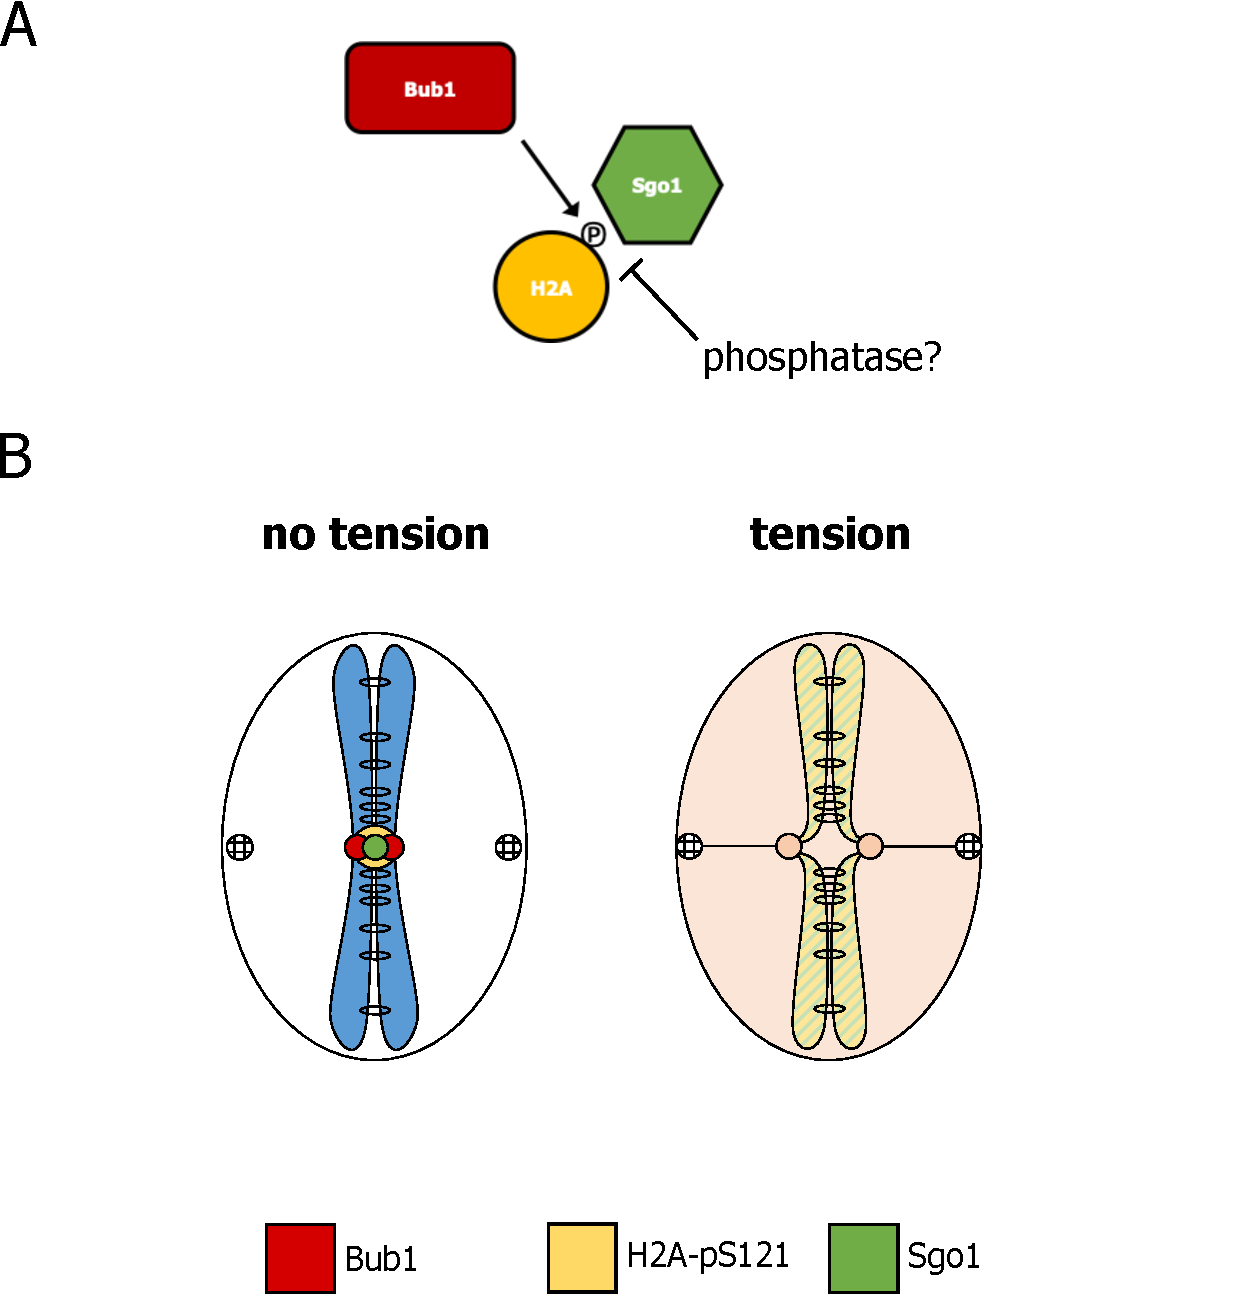
\includegraphics[width=0.9\textwidth]{chapter3/figures/graphic_model_final.pdf}
  \caption[Schematics of tension-dependent re-localisation of Sgo1]{Schematics of tension-dependent re-localisation of Sgo1. (A) Molecular machinery determining the localisation of Sgo1. The balance between Bub1 kinase and an unknown phosphatase determines the phosphorylation level of H2A at serine 121 and thus Sgo1 recruitment. (B) Spatial regulation of Bub1, H2A-pS121 and Sgo1 by tension. In the absence of tension, Bub1 is localised at the kinetochores and locally phosphorylates H2A at the peri-centromeric region, which then recruits Sgo1 to the peri-centromere. Upon the establishment of tension, Bub1 diffuses away from the kinetochore and reaches chromatin outside the peri-centromere, shifting the local kinase-phosphatase balance at both places. This leads to the H2A-S121 de-phosphorylation at the peri-centromere but phosphorylation at other parts of the genome, which titrates Sgo1 away from the peri-centromere.}
  \label{fig:finalmodel}
\end{figure}

This model (Figure~\ref{fig:finalmodel}B) processes the same notion as the yeast model proposed by \cite{Nerusheva2014} that opposing kinase and phosphatase are at the core of Sgo1 tension-dependent re-localisation. However, the details of the two models are rather different. \cite{Nerusheva2014} model proposes that tension increases the distance between kinetochore-localised Bub1 and its non-H2A-S121 substrate at the peri-centromere, leading to the de-phosphorylation by Sgo1-bound PP2A-Rts1 and eventually Sgo1 de-localisation. The differences between the two models majorly arise for three reasons. First, the analyses of G1-to-metaphase Bub1 live-cell imaging are different. \cite{Nerusheva2014} classified cells with the criteria that whether the Bub1 foci were visible by eye. Due to the persistence of Bub1 foci, the result was interpreted as Bub1 being removed from the kinetochore much later than Sgo1 re-localisation, leading to the hypothesis that kinetochore-bound Bub1 is pulled away from its substrate by tension. Whereas in this study, the fluorescence intensity of Bub1 foci was further quantified, which showed a sharp decrease around the same time, if not slightly earlier, when Sgo1 is re-localised. This observation brought up the possibility that Bub1 kinetochore localisation itself could be regulated by tension and it triggers downstream de-phosphorylation, which is revealed in the model proposed in this study. Second, the two models disagree on whether H2A-S121, the known Bub1 substrate important for Sgo1 localisation, is the key substrate regulated in the process. As mentioned above, a likely strain confusion gave rise to the interpretation that Bub1 substrate other than H2A-S121 is the key to Sgo1 re-localisation in \cite{Nerusheva2014}. However, with re-constructed strains, experiments conducted in this study suggested the opposite. Third, \cite{Nerusheva2014} model recognises PP2A-Rts1 as the phosphatase de-phosphorylating Bub1 substrate because the Sgo1 ChIP signal at peri-centromere was increased in the absence of tension and that the duration of Sgo1 foci was increased by 15 \si{\minute} in \textit{rts1$\Delta$}. Nevertheless, repeating the imaging experiment in this study did not show higher fluorescence intensities of Sgo1 foci in \textit{rts1$\Delta$}, asking for an alternative interpretation of the ChIP data. Detailed analysis of inter-kinetochore distance indicated a similar value at which Sgo1 foci are dispersed between \textit{rts1$\Delta$} and the wild type, suggesting the delay observed in \cite{Nerusheva2014} was probably due to reduced tension. 

The human model for tension-dependent re-localisation of Sgo1 describes a very different picture \citep{Liu2013a}. In the model, upon the establishment of tension, Sgo1 is de-phosphorylated at T346 by an unknown phosphatase, which switches it from cohesin-bound to H2A-pT120-bound. Given that cohesin is enriched at the inner centromere while H2A-pT120 is proximal to the kinetochore, Sgo1 moves from the inner centromere towards the kinetochore-proximal chromatin. However, there is evidence suggesting that the yeast model proposed in this study (Figure~\ref{fig:finalmodel}B) could also be conserved in humans. The key event of our yeast model is the re-distribution of H2A-pS121, the yeast equivalent of human H2A-pT120. Interestingly, in humans, disruption of the kinetochore localisation of Bub1, either by a point mutation \citep{Asghar2015} or by fusing the Bub1 kinase domain to BubR1, which allows the kinase domain to be part of the diffusible MCC complex \citep{Wang2022SpatialMitosis}, could lead to a similar spread of H2A-pT120 to the chromosome arms. Notably, in both cases, the centromeric localisation of shugoshin proteins was comprised. Although \cite{Liu2013a} showed that H2A-pT120 remains at kinetochore-proximal chromatin under tension, \cite{Asai2020} reported a decrease in the IF intensities of H2A-pT120. It is possible that the difference here resembles what has been discussed above about the different interpretations of Bub1 live-cell imaging. Moreover, centromeric Bub1 and Sgo2 were reported to decrease upon tension in that research \citep{Asai2020}. Therefore, the sequential de-localisation of Bub1, H2A-pT120 and shugoshins might also exist in humans. A unified model can be proposed in combination with \cite{Liu2013a} model. Potentially, in human cells, tension both de-localises Bub1 from the kinetochore and de-phosphorylates Sgo1, resulting in the majority of Sgo1 being moved to chromosome arms while a small but observable portion remaining at the centromeric region. This might also be true in budding yeast, as residual Bub1 \citep{Nerusheva2014, Bokros2021YeastAnaphase}, H2A-pS121 (this study) and Sgo1 \citep{Paldi2020ConvergentPericentromeres} have been observed at the old locations after their re-distributions upon tension. 

The major limitation of the proposed model (Figure~\ref{fig:finalmodel}B) lies in the unidentified phosphatase. Using general phosphatase inhibitors might be a good start to test the idea. Nevertheless, various difficulties and artefacts from cell death, yeast cell wall and changed pH of media were encountered in those experiments, which will not be elaborated on here. Apart from it, a final proof of this model would be showing that Sgo1 is indeed localised at chromosome arms once tension is established. In favour of this idea, over-expressed Sgo1 can be detected on chromosome arms by ChIP in cycling budding yeast and the enrichment is largely dependent on Bub1 \citep{Clift2009}. However, available Sgo1 ChIP-seq in the presence or absence of tension did not show an obvious difference in arm enrichment \citep{Paldi2020ConvergentPericentromeres}. Yet, it is worth noting that this ChIP-seq was not calibrated and that the Sgo1 ChIP signal is barely distinguishable from noise due to its low protein abundance and the fact that it does not directly bind DNA. Because of the undissolved nuclear envelope of budding yeast in mitosis, it is unable to distinguish chromosome arm localisation from nuclear localisation by microscopy, leaving a direct test of the hypothesis challenging. 

Shugoshin has been proposed as the tension sensor which translates the mechanical force into biochemical signals that can be read by the cell \citep{Indjeian2005a, Nerusheva2014, Marston2015}. However, the sole dependence of Sgo1 localisation on Bub1 localisation found in this study makes it rather a signal transducer. Indeed, shugoshin processes feature beneficial for this role. Positive feedback of its own localisation has been reported in human cells \citep{Liang2019ACells} and budding yeast \citep{Roy2019}, which gives Sgo1 the potential to respond quickly to a signal. How is tension sensed by the cells then? Extensive research has been conducted and various, not necessarily mutually exclusive models have been proposed on this topic \citep{Hindriksen2017TheLocalization, McVey2021AuroraSegregation, Broad2020AuroraCells}. Data obtained in this study are in line with the model proposed by \cite{Roy2019} that PP1 is recruited to Spc105 (Knl1) upon tension to de-phosphorylate the MELT motifs and thus release Bub1. In support of this idea, human Knl1 has been reported to undergo conformational changes when tension is established \citep{Roscioli2020}. 

Further work is required to validate the yeast model proposed here. To draw a final conclusion about whether PP1 has a role in de-phosphorylating H2A-pS121, a time course experiment followed by H2A-pS121 western blotting, similar to Figure~\ref{fig:ph2abub1aid}, in PP1 temperature-sensitive mutants could be performed. Although suffered from the sub-optimal signal-to-noise ratio, it might still be worth conducting a calibrated Sgo1 ChIP-seq to distinguish whether Sgo1 is localised to chromatin arms or is dispersed to the nucleus after re-localisation. More advanced ChIP-seq-like technologies, such as CUT\&RUN sequencing, could also be considered. As for the human model of Sgo1 tension-dependent re-localisation, it is important to quantify the amount of Bub1, H2A-pT120 and shugoshins at centromeric regions, possibly by IF, before and after tension. Given the release of T2T \citep{Nurk2022TheGenome}, the first complete human reference genome that can cover the centromeres, sequencing-based technologies could also be applied to investigate the question now. 

\nomenclature{T2T}{Telomere-to-Telomere}
\nomenclature{MCC}{Mitotic Checkpoint Complex}

\subsection{The regulation of Bub1 localisation potentially links chromosome condensation to SAC status}

Chromosome condensation is an essential step in mitosis and meiosis for accurate segregation \citep{Antonin2016ChromosomeMitosis, Piskadlo2016NovelCondensation, Beseda2020MitoticVariability, Takahashi2019FoldingChromosomes}. In budding yeast, it has been shown that Bub1, H2A-pS121 and Sgo1 are required for chromosome condensation in anaphase \citep{Kruitwagen2018}. However, the molecular mechanism is unclear. Important players in chromosome condensation, including condensin, CPC and topoisomerase II, were reported to interact with either shugoshin or the H2A phosphorylation \citep{Zhang2020FunctioningMitosis, Verzijlbergen2014, Yahya2020, Abad2022MechanisticCPC}. The finding that H2A-pS121, and possibly Sgo1, spreads from centromeres to chromosome arms by tension brings up the hypothesis that these re-distributions might facilitate the spread of the important effectors for chromosome condensation to initiate the process. If the hypothesis is true, one would anticipate chromosome condensation to happen upon the establishment of tension. Indeed, compared to the tension-less situation, the Hi-C map of metaphase cells with tension indicated mild characteristics of chromosome condensation (Figure~\ref{fig:Hi-C+-tension}). 

This observation has not been reported before. It suggested a possible model for chromosome condensation in budding yeast, where tension disperses Bub1 from the kinetochore, releases H2A-pS121 and hence Sgo1 to the chromosome arms, which brings condensin, CPC or Top2 with them, and eventually leads to chromosome condensation (Figure~\ref{fig:ultimatemodel}). In support of the hypothesis, \cite{Leonard2015} showed that condensin has a similar centromere-to-arm re-distribution when cells are released from tension-less to tension situation by ChIP-qPCR. Besides, they also found an increase in Top2 association with arms but not centromeres over time upon a tension-less release. Interestingly, given Bub1 de-localisation being the hallmark of SAC silencing, the hypothesis potentially links chromosome condensation to a cell cycle checkpoint. Moreover, chromosome condensation has been recognised as reaching its maximum in early anaphase\cite{Antonin2016ChromosomeMitosis}. The model proposed above could challenge it with the idea that the maximum might be reached in late metaphase. 

It is not known, though, whether this tension-dependent chromosome condensation requires Bub1, H2A-pS121 and Sgo1. The question could be answered by Hi-C performed on null or phospho-null mutants in the presence and absence of tension. The H2A phospho-null mutant used in this study was generated by deleting both H2A subtypes and supplying the cell with plasmids expressing the mutated one. To rule out the possibility of altered H2A expression affecting chromosome conformation, the H2A phospho-mutant to be used in the Hi-C experiments could be made by mutating both subtypes \textit{in situ}. If the necessity is validated, the effector(s) involved then needs to be identified. Calibrated ChIP-seq of cells with or without tension could be conducted for condensin, CPC/H3-pS10 and Top2 to investigate if they show a similar re-distribution. One would expect the true effector(s) to do so. If it is identified, the final proof of the model would be to show the dependence of the effector's re-distribution on Sgo1 or H2A-pS121, for which ChIP-seq could also be used. \cite{Kruitwagen2015} reported that chromosome condensation is autonomous, which is against the assumption of our model that Bub1 diffuses to arms after being de-localised from the kinetochore. It would be interesting to repeat the result as well. 

\begin{figure}[htbp]
  \centering
  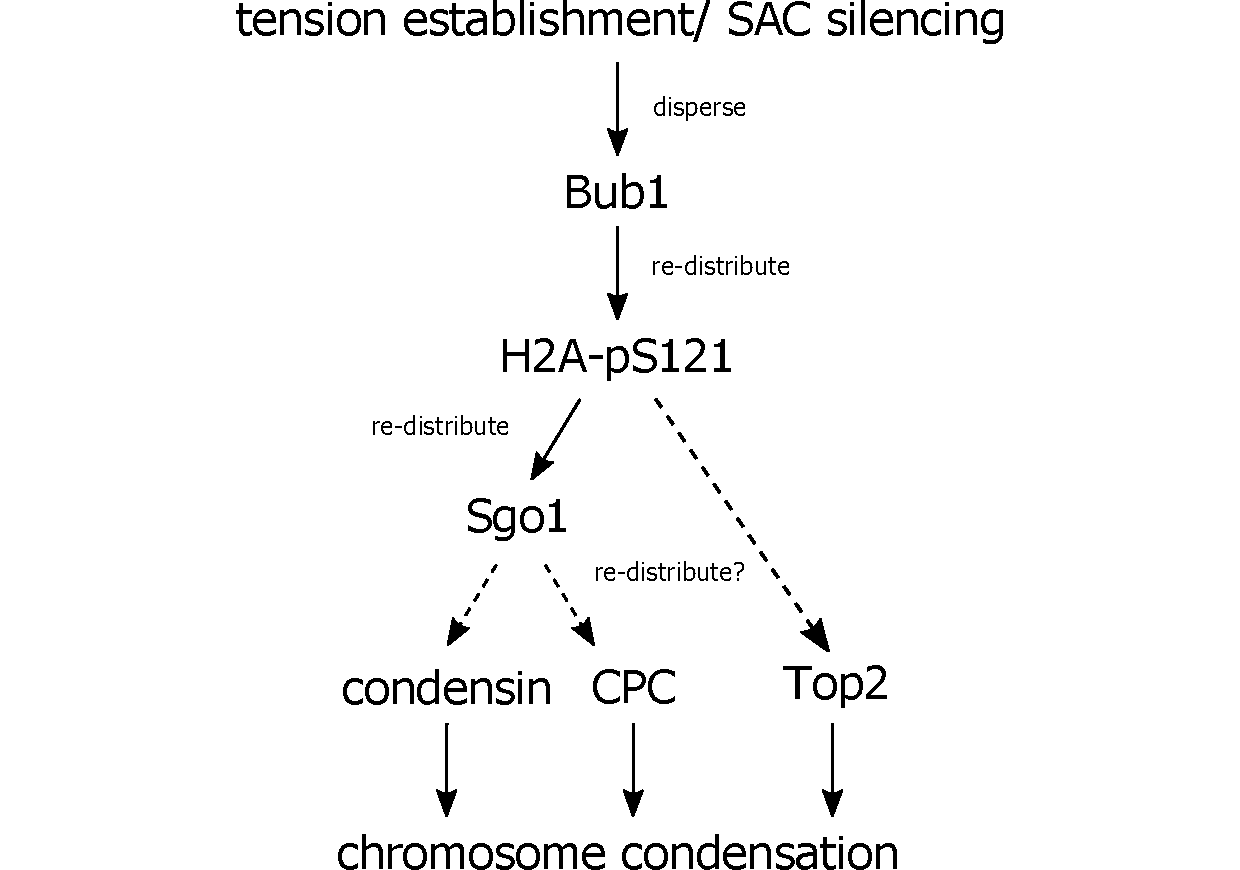
\includegraphics[width=0.9\textwidth]{chapter3/figures/ultimate_model.pdf}
  \caption[Hypothetical model for the role of Sgo1 in chromosome condensation]{Hypothetical model for the role of Sgo1 in chromosome condensation. The establishment of tension de-localises Bub1 from the kinetochore, leading to the spreading of H2A and Sgo1 from centromeres to chromosome arms. This might result in the re-distribution of condensin, CPC, Top2, or possibly combinations of them to the arms and hence chromosome condensation. }
  \label{fig:ultimatemodel}
\end{figure}

\subsection{The role of cohesin in localising Sgo1}

Shugoshin was discovered for its role in protecting centromeric cohesin from the cleavage by separase during metaphase I \citep{Kerrebrock1992TheDifferentiation, Marston2004a, Kitajima2004a, Katis2004, Rabitsch2004TwoII}. Consistent with intuition, the existence of physical interaction between Sgo1 and cohesin has been established in human cells \citep{Tanno2009}. It is later found that cohesin is important for Sgo1 localisation to the inner centromere \citep{Liu2013a}. Whether the dependence of Sgo1 localisation on cohesin is conserved in budding yeast is unknown. But there was evidence in favour of conservation. Sgo1 ChIP-seq showed three local maxima at the core centromere and two borders of peri-centromere on each chromosome, corresponding well with cohesin profiles in this region \citep{Deng2018TripartiteChromosomes}. Upon cohesin depletion, ChIP-qPCR signals of Sgo1 at the centromeric regions were massively reduced \citep{Verzijlbergen2014}. Moreover, H2A-pS121 processes a bell-shaped rather than a tripartite profile, implying the involvement of other factors in localising Sgo1 (Figure~\ref{fig:sgo1comparison}). This study attempted to answer the question by performing Sgo1 live-cell imaging upon cohesin depletion. Unexpectedly, Sgo1 foci were still formed and maintained till the end of the experiment, suggesting that cohesin is, at least, not required for the enrichment of Sgo1 at the centromeric region. 

This result is surprising given the evidence above implying cohesin is important for Sgo1 localisation. But it does agree with the experiment by \cite{Indjeian2005a} where they found Sgo1 is required for the cell cycle delay induced by cohesin depletion. One possibility that can explain the contradiction is that cohesin is required for fine but not coarse localisation of Sgo1 as in human cells, which cannot be detected with the current resolution of the microscope due to the small size of budding yeast. 

To test the possibility, methods with higher resolution, such as ChIP-seq, should be used. But sequence-based methods might require extra care when combined with cohesin depletion as it could affect chromosome conformation and complicate the interpretation. An alternative method could be to obtain structural data of the Sgo1-cohesin complex first and find amino acids important for the interaction. Then sequence-based methods can be applied to mutants whose Sgo1-cohesin interaction was specifically abolished by point mutations. 

\subsection{PP2A could regulate Sgo1 functions}

Shugoshin has been reported to be phospho-regulated in various species \citep{Llano2008Shugoshin-2Mice, Tanno2010, Rattani2013Sgol2Oocytes, Pouwels2007ShugoshinPlk1, Kawashima2007, Lee2014RegulationPhosphorylation, Liu2013, Liu2013a, Clarke2005, Resnick2006INCENPDrosophila, Nogueira2014, Yahya2020}. As a phosphatase that interacts with shugoshin, PP2A-B56 might regulate its phosphorylation. In support of the hypothesis, Sgo1 IP-MS in \textit{rts1$\Delta$} showed an altered Sgo1 phosphorylation, with amino acid 418-433 increased whereas amino acid 484-494 decreased. 

Different work could be carried out to follow up on this preliminary result. Due to not being in direct relevance to this study, whether these regions are truly phosphorylated and regulated by PP2A-Rts1 remained untested. Phospho-specific antibodies might be considered for this purpose. If they are verified, it is then important to understand their functional relevance. Given the major function of shugoshin, one could start with screening for defects in chromosome segregation in point mutants of potential phospho-sites in the regions mentioned above. It is surprising that in the absence of PP2A-Rts1, Sgo1 had reduced phosphorylation at amino acid 484-494. It would be intriguing to understand the underlying mechanism. One possibility is PP2A-Rts1 might up-regulate the activity of the kinase(s) phosphorylating Sgo1. Alternatively, PP2A-Rts1 binding to Sgo1 could physically mask the region. Albeit the conventional opinion that PP2A-Rts1 binds Sgo1 at its coiled-coil domain, this hypothesis is supported by the recent finding in human cells that Sgo1 has additional interacting surface(s) with PP2A-B56. 

\section{Materials and methods}

\subsection{General information}
\subsubsection{Supplier information}
Chemicals and reagents used in this study, unless otherwise stated, were from suppliers including Abcam, Beckman, Bioo Scientific, Biorad, GenScript Biotech, Gibco BRL, Illumina, Invitrogen, Melford, Merck, New England Biolabs, Promega, Qiagen, Scientific Laboratory Supplies, TAKARA BIO INC., Thermo Fisher Scientific. 

Growth media reagents used in this study were supplied by Difco, Formedium and Sigma. 
\subsubsection{Sterilisation}
Glassware was sterilised by dry heat treatment using a hot air oven at 250 \si{\celsius} for 16 \si{\hour}. Chemical solutions were sterilised by filtration through Nalgene 0.2 \si{\micro\metre} PES membrane rapid-flow bottle top filters or through Millex-GP 0.22 \si{\micro\metre} PES membrane syringe filter unit. Growth media was sterilised by autoclaving at 120 \si{\celsius} for 15 \si{\minute}. 

\nomenclature{PES}{PolyEtherSulfone}
\subsection{Bacterial methods}
\subsubsection{Bacterial media and drugs}
\underline{LB media}\\ 
1 \% w/v Bacto-tryptone \\ 
0.5 \% w/v Bacto-yeast extract \\ 
0.5 \% w/v NaCl \\ 
Adjusted to pH 7.2 with NaOH \\
For plate use, 2 \% w/v agar was additionally added. \\

\underline{SOC media}\\
2 \% w/v Bacto-tryptone \\ 
0.5 \% w/v Bacto-yeast extract \\ 
20 \si{\milli\Molar} NaCl \\
20 \si{\milli\Molar} Glucose \\
10 \si{\milli\Molar} MgCl$_{2}$ \\
10 \si{\milli\Molar} MgSO$_{4}$ \\
10 \si{\milli\Molar} KCl \\

\underline{Ampicillin}\\
Stock: 100 \si{\milli\gram/\milli\litre} in water \\
Working concentration: 100 \si{\micro\gram/\milli\litre} 

\nomenclature{LB}{Luria-Bertani}
\nomenclature{SOC}{Super Optimal broth with Catabolite repression}

\subsubsection{Bacterial growth}
\textit{E.coli} was grown with either solid or liquid media. For solid media, strains were plated on LB agar containing Ampicillin and placed at 37 \si{\celsius} overnight. For liquid media, strains were inoculated into LB media containing Ampicillin and incubated at 37 \si{\celsius} with shaking at 200 rpm overnight. 

\subsubsection{Bacterial storage}
For long-term storage, the overnight-grown liquid culture of cells with 20 \% w/v glycerol was stored in a cryovial at -80 \si{\celsius}. For short-term storage, cells could be placed on plates at 4 \si{\celsius} for up to 2 weeks. 

\subsubsection{Chemically competent DH5$\alpha$ \textit{E.coli} transformation}
\underline{TFB1} \\
100 \si{\milli\Molar} RbCl \\
50 \si{\milli\Molar} MnCl$_{2}$ \\ 
30 \si{\milli\Molar} potassium acetate\\
10 \si{\milli\Molar} CaCl$_{2}$\\
15 \% w/v glycerol\\
pH to 5.8 with 1.75 \si{\Molar} Acetic Acid\\

\underline{TFB2} \\
10 \si{\milli\Molar} MOPS\\
10 \si{\milli\Molar} RbCl\\
75 \si{\milli\Molar} CaCl$_{2}$\\
15 \% w/v glycerol\\
pH slowly to 6.5 with 2 \si{\Molar} KOH 2-4 \si{\milli\litre}\\

Revived DH5$\alpha$ \textit{E.coli} strain was inoculated into LB liquid media and grown at 37 \si{\celsius} overnight. In the following morning, the culture was diluted 1:200 with pre-warmed LB media supplemented with 20 \si{\milli\Molar} MgSO$_{4}$. After reaching $OD_{600}$=0.48, cells were incubated for 10 \si{minute} on ice and harvested by centrifuging for 5 \si{\minute} at 5000 rpm at 4 \si{\celsius}. They were then washed with TFB1 and resuspened in TFB2 at 10$^{9}$ CFU/\si{\milli\litre}. Chemically competent cells were later stored at -80 \si{\celsius}. 

50 \si{\micro\litre} aliquot of competent cells was thawed on ice and mixed with 3 \si{\micro\litre} of plasmid DNA, from Gibson assembly or plasmid preparation using lab protocol, by gently flicking. After incubating for 30 \si{\minute} on ice, \textit{E.coli} cells were heat-shocked at 42 \si{\celsius} for 30 \si{\second} and placed on ice for 5 \si{\minute}. Next, 450 \si{\micro\litre} of pre-heated SOC media was added. The cell culture was then incubated at 37 \si{\celsius} with shaking at 200 rpm for 1 \si{\hour} for the recovery of \textit{E.coli}. Afterwards, 100 and 400 \si{\micro\litre} of cell culture were plated on solid LB media to grow for single colonies. 

\nomenclature{MOPS}{3-(N-Morpholino)PropaneSulfonic acid}
\nomenclature{CFU}{Colony-Forming Unit}
\nomenclature{TFB}{Transformation Buffer}

\subsection{Budding yeast methods}
\subsubsection{Budding yeast media and drugs}
\underline{YPDA media} \\
1 \% w/v Bacto-yeast extract \\
2 \% w/v Bacto-peptone \\
2 \% w/v Glucose \\
0.3 \si{\milli\Molar} Adenine \\
For plate use, 2 \% w/v agar was additionally added. \\

\underline{SC media} \\
1 \% w/v yeast nitrogen base without amino acid \\
200 \si{\milli\gram/\litre} all amino acids that comprise proteins except Leucine \\
400 \si{\milli\gram/\litre} Leucine \\
200 \si{\milli\gram/\litre} Uracil \\
20 \si{\milli\gram/\litre} PABA \\
2 \% w/v Glucose \\ 
0.3 \si{\milli\Molar} Adenine\\
For plate use, 2 \% w/v agar was additionally added. \\

\nomenclature{PABA}{p-Amino Benzoic Acid}

\underline{CSM drop-out media} \\
1 \% w/v yeast nitrogen base without amino acid \\
1 x Formedium CSM without specific amino acid(s)\\
2 \% w/v Glucose \\ 
0.3 \si{\milli\Molar} Adenine\\
For plate use, 2 \% w/v agar was additionally added. \\
IMPORTANT: CSM -MET plates have to be fresh for single-cell growth uses, including dissection, transformation and streaking. \\

\underline{SPO media}\\
1 \% w/v Potassium acetate\\
200 \si{\milli\gram/\litre} all amino acids that comprise proteins except Leucine \\
400 \si{\milli\gram/\litre} Leucine \\
200 \si{\milli\gram/\litre} Uracil \\
200 \si{\milli\gram/\litre} Adenine\\
20 \si{\milli\gram/\litre} PABA \\
For plate use, 2 \% w/v agar was additionally added. \\

\underline{$\alpha$ factor}\\
Stock: 5 \si{\milli\gram/\milli\litre} in DMSO \\
Working concentration: 5 \si{\micro\gram/\milli\litre}\\

\underline{Benomyl} \\
Stock: 30 \si{\milli\gram/\milli\litre} in DMSO \\ 
Working concentration: 30 \si{\micro\gram/\milli\litre}, unless otherwise stated \\
Benomyl stock solutions have to be added to boiling hot liquid media to dissolve. \\

\underline{Nocodazole}\\
Stock: 1.5 \si{\milli\gram/\milli\litre} in DMSO \\
Working concentration: 15 \si{\micro\gram/\milli\litre} \\

\underline{Geneticin (G418)} \\ 
Geneticin was used to select for KanMX6 marker.\\
Working concentration: 250 \si{\micro\gram/\milli\litre} for YPDA plates.\\

\underline{Hygromycin-B}\\
Hygromycin-B was used to select for HphMX marker.\\
Working concentration: 400 \si{\micro\gram/\milli\litre} for YPDA plates.\\

\underline{Nourseothricin (CloNAT)}\\
Nourseothricin was used to select for NatMX marker. \\
Working concentration: 100 \si{\micro\gram/\milli\litre} for YPDA plates.\\

\subsubsection{Budding yeast growth}
\underline{Vegetative growth}\\
w303 strains stored at -80 \si{\celsius} freezers were revived by patching frozen cell culture onto appropriate plates and placing them at 30 \si{\celsius} overnight. For growth in liquid media, cells were inoculated into flasks with media less than 20 \% of their maximal capacities and incubated at RT with shaking at 250 rpm. \\

\underline{G1 arrest by $\alpha$ factor}\\
Overnight-grown w303 strains in appropriate media were diluted to $OD_{600}$=0.2 and incubated at RT with shaking at 250 rpm for over 1 \si{\hour} to allow them to enter exponential growth. Afterwards, cells were re-diluted to $OD_{600}$=0.2. $\alpha$ factor was then added at 5 \si{\micro\gram/\milli\litre}. 1.5 \si{\hour} later, additional $\alpha$ factor was added at 2.5 \si{\micro\gram/\milli\litre} and cells were incubated for another 1.5 \si{\hour}.\\

\underline{Metaphase arrest with tension by \textit{pMET-CDC20}}\\
G1 arrested w303 strains bearing \textit{pMET-CDC20} were washed out for $\alpha$ factor and released into SC (for microscopy experiments) or YPDA (for other experiments) media with an additional 8 \si{\milli\Molar} methionine for 2 \si{\hour}. 4 \si{\milli\Molar} methionine was re-added 1 \si{\hour} since the release. \\

\underline{Metaphase arrest without tension by nocodazole}\\
G1 arrested w303 strains were washed out for $\alpha$ factor and released into SC (for microscopy experiments) or YPDA (for other experiments) media with 15 \si{\micro\gram/\milli\litre} nocodazole for 2 \si{\hour}. 7.5 \si{\micro\gram/\milli\litre} nocodazole was re-added 1 \si{\hour} since the release.

Due to the large scale of the Sgo1 IP-MS experiment, benomyl at 30 \si{\micro\gram/\milli\litre} was used to induce metaphase arrest without tension. \\

\underline{Metaphase arrest with cohesin depleted by \textit{pMET-SCC1}}\\
The procedure is identical to metaphase arrest with tension by \textit{pMET-CDC20} except 8 \si{\milli\Molar} methionine was added 45 \si{\minute} before the release from $\alpha$ factor arrest to pre-clean Scc1. \\

\subsubsection{Budding yeast storage}
For long-term storage, overnight-grown yeast cells from patches on appropriate plates were resuspended in 20 \% w/v glycerol and stored in cryovials at -80 \si{\celsius}. For short-term storage, cells were placed on appropriate plates at 4 \si{\celsius} for up to several weeks.

\subsubsection{High-efficiency budding yeast transformation}

\underline{LiTE}\\
100 \si{\milli\Molar} LiAc pH 7.5 \\
10 \si{\milli\Molar} Tris-HCl pH 7.5 \\ 
1 \si{\milli\Molar} EDTA pH 7.5 \\

\underline{40 \% PEG solution}\\
40 \% w/v PEG4000\\
100 \si{\milli\Molar} LiAc pH 7.5\\
10 \si{\milli\Molar} Tris-HCl pH 7.5\\
1 \si{\milli\Molar} EDTA pH 7.5\\

\underline{TE}\\
10 \si{\milli\Molar} Tris-HCl pH 7.5\\
1 \si{\milli\Molar} EDTA pH 7.5\\

Modified from \cite{Gietz2007High-efficiencyMethod}. Overnight-grown w303 strains in appropriate media were diluted to $OD_{600}$=0.2 and incubated at 30\si{\celsius} with shaking at 250 rpm. Cells were harvested at $OD_{600}$=0.3-1.0 by centrifuging at 3000 rpm for 3 \si{\minute}. Sequentially washed by distilled water and LiTE, cells of 10 \si{\milli\litre} culture were then resuspended in 50 \si{\micro\litre} of LiTE. 300 \si{\micro\litre} of 40 \% PEG solution, 10 \si{\micro\litre} of ssDNA and the DNA of interest was mixed with the 50 \si{\micro\litre} of yeast suspension. Next, the mixture was incubated at 30 \si{\celsius} with shaking at 250 rpm for 30 \si{\minute}. Afterwards, 
yeast cells were heat-shocked at 42 \si{\celsius} for 15 \si{\minute}. Finally, they were resuspended in 200 \si{\micro\litre} of TE and plated onto appropriate selection plates. If a drug-resistant selection mark was used, cells were first plated onto YPDA plates for 24 \si{\hour} and then replica plated onto the corresponding drug-containing plates to allow time for expressing drug-resistant proteins.

\nomenclature{PEG}{PolyEthylene Glycol}
\nomenclature{EDTA}{EthyleneDiamineTetraacetic Acid}

\subsubsection{Crossing haploid budding yeast}

w303 haploids of opposite mating types were mixed on appropriate plates and incubated for over 8 \si{\hour} at 30 \si{\celsius}, with MAT$\alpha$ in small quantity while MATa in large quantity. The mix was then streaked to single colonies and incubated at 30 \si{\celsius}. To select for diploids. 40 \si{\micro\litre} of 5 \si{\milli\gram/\milli\litre} $\alpha$ factor was used to prevent the growth of haploid MATa cells. If applicable, the selection marker present in MATa but not in MAT$\alpha$ strain could be used to prevent the growth of haploid MAT$\alpha$ cells. After colonies were formed, usually around 48 \si{\hour}, cells from single colonies were patched onto YPDA plates and incubated at 30 \si{\celsius} overnight. Patches were then transferred onto SPO plates and incubated at 30 \si{\celsius} for over 48 \si{\hour} to induce sporulation for dissection. 

\subsubsection{Budding yeast tetrad dissection}

\underline{Tetrad digestion mix}\\
1 \si{\milli\gram/\milli\litre} AMS biotechnology Zymolase\\
2 \si{\Molar} Sorbitol \\

A small amount of sporulated diploid cells was added to 20 \si{\micro\litre} of tetrad digestion mix and incubated at RT for 8 \si{\minute} to degrade the cell wall. Afterwards, 1 \si{\milli\litre} of distilled water was added to stop digestion. Yeast suspension was then transferred onto appropriate plates for tetrad dissection, which was performed under a Singer MSM 400 Dissection Microscope according to the user manual. Dissected single haploid cells were incubated at 30 \si{\celsius} for over 48 \si{\hour} to allow colony formation. 

\subsubsection{Budding yeast spot assay}

Lab Bunsen burner was used for sterilisation. For a 1:5 serial dilution, 160 \si{\micro\litre} of distilled water was added to each well of a 96-well plate by a multi-channel pipette. An additional 40 \si{\micro\litre} of distilled water was added to the first column. Revived budding yeast cells were then added to the wells of the first column. The 1:5 serial dilution was performed using the multi-channel pipette. A replica plater, sterilised by burning ethanol using the Bunsen Burner, was used to dip cell cultures in the 96-well plates and transferred them to the appropriate plates. The plates were then incubated at temperatures according to the experiment design. A scanner was used to acquire photos of the plates. 

\subsection{Fission yeast methods}
\subsubsection{Fission yeast media and drugs}

\underline{YES}\\
0.5 \% w/v bacto-yeast extract\\
3 \% w/v glucose\\ 
0.02 \% w/v Adenine\\ 
0.02 \% w/v Histidine\\
0.02 \% w/v Leucine\\ 
0.02 \% w/v Uracil \\ 
0.02 \% w/v Lysine \\
For plate use, 2 \% w/v agar was additionally added.

\subsubsection{Fission yeast growth}

\underline{Vegetative growth}\\
972 h$^{-}$ strains stored at -80 ◦C freezers were revived by patching frozen cell culture onto appropriate plates and placing them at 30 ◦C overnight. Revived cells were inoculated into the appropriate liquid media and incubated at 30 \si{\celsius} for 8 \si{\hour} with shaking at 250 rpm. The cell culture was subsequently diluted to OD$_{600}$=0.01 and grown overnight. In the following morning, the cell culture was diluted to OD$_{600}$=0.1 and incubated at 30 \si{\celsius} with shaking at 250 rpm until desired OD$_{600}$ was reached. 

\subsection{Microscopy methods}
\subsubsection{Sensitised Emission FRET}
Sensitised Emission FRET experiments were performed on a Nikon Ti2 inverted microscope equipped with a 100x Plan ApoChromat NA 1.45 oil lens and a Prime 95B CMOS (sCMOS) camera. The protocol was modified from \cite{Gordon1998QuantitativeMicroscopy}. Three strains, acceptor only, donor only and FRET (contains both acceptor and donor), were constructed and prepared for imaging. To correct for the bleed-through from acceptor and donor to the FRET channel, the following co-efficiencies were calculated in advance using the acceptor only or donor only strain:
\begin{align*}
    & \text{co-efficient A}& =\frac{\text{Mean intensity}_\text{Acceptor in FRET channel}}{\text{Mean intensity}_\text{Acceptor in Acceptor channel}}\\
    &\\
    & \text{co-efficient B}& =\frac{\text{Mean intensity}_\text{Donor in FRET channel}}{\text{Mean intensity}_\text{Donor in Donor channel}}
\end{align*}

For the FRET sample, the FRET channel was recorded first. The donor and acceptor channels were subsequently applied. The FRET signal of each pixel was corrected in imageJ using the following formula: 

\begin{align*}
    \text{corrected FRET intensity} &= \text{Intensity}_\text{FRET channel}\\& - \text{co-efficient A} \times \text{Intensity}_\text{Acceptor channel}\\& - \text{co-efficient B} \times \text{Intensity}_\text{Donor channel}
\end{align*}

\subsubsection{Live-cell imaging using 8-well Ibidi dishes on the Zeiss microscope}

\underline{Concanavalin A solution}\\
5 \si{\milli\gram/\milli\litre} Concanavalin A \\
50 \si{\milli\Molar} CaCl$_{2}$ \\
50 \si{\milli\Molar} MnCl$_{2}$ \\

Cells bearing \textit{pMET-CDC20} from patches on -MET plates were inoculated in 10 \si{\milli\litre} of CSM -MET media and incubated at RT with shaking at 250 rpm overnight. Cells were diluted to $OD_{600}$=0.2 in 10 \si{\milli\litre} of CSM -MET in the morning, incubating at RT with shaking at 250 rpm for over 1 \si{\hour}, allowing cells to enter the exponential phase. Then, cells were re-diluted to $OD_{600}$=0.2 in 10 \si{\milli\litre} of CSM -MET and 10 \si{\micro\litre} of 5 \si{\milli\gram/\milli\litre} $\alpha$ factor was added for G1 synchronization. After 1.5 \si{\hour}, another 5 \si{\micro\litre} of 5 \si{\milli\gram/\milli\litre} $\alpha$ factor was added. 1.5 \si{\hour} later, shmoo morphology was checked by a light microscope to ensure G1 arrest. 1 \si{\milli\litre} of cell culture was transferred to a 1.5 \si{\milli\litre} Eppendorf tube and concentrated by centrifuging at 3000 rpm for 3 \si{\minute} then removing 700 \si{\micro\litre} of supernatant. 250 \si{\micro\litre} of concentrated cell culture was loaded onto an 8-well Ibidi dish pre-treated with concanavalin A and incubated at RT on bench for 15 \si{\minute} to allow cells to bind the bottom of the dish. The supernatant was removed using a bench aspirator and cells were washed twice with 250 \si{\micro\litre} of SC media. After the final wash, 250 \si{\micro\litre} of SC media was added to each well for imaging. 

Live-cell imaging experiments were performed on a Zeiss Axio Observer inverted microscope equipped with a 100x alpha-Plan ApoChromat NA 1.46 oil lens and a Hamamatsu Orca Flash 4 V2 camera. Experimental settings varied according to the requirements of different experiments. A representative example is provided for strains carrying \textit{SGO1-EGFP} \textit{MTW1-tdTomato}. The imaging was carried out at 25 \si{\celsius} for 3 \si{\hour}, with an imaging interval of 15 \si{\minute}. 5 fields were imaged for each strain with 13 0.5-\si{\micro\metre} Z slices. For the GFP channel, 10 \% 469/38 \si{\nano\metre} LED Light Source was used to excite Sgo1-EGFP and the emission was received at 525/50 \si{\nano\metre} with an exposure time of 150 \si{\milli\second}. For the tdTomato channel, 5 \% 555/30 \si{\nano\metre} LED Light Source was used to excite Sgo1-EGFP and the emission was received at 605/70 \si{\nano\metre} with an exposure time of 150 \si{\milli\second}. 

The AID system can be used for inducible protein degradation in live-cell imaging. But the concentration of NAA should be kept as low as 100 \si{\micro\Molar} because blue light, the exciting light for the GFP channel, accelerates the oxidative de-carboxylation of auxin, which causes cytotoxicity to budding yeast \citep{Papagiannakis2017QuantitativeCells}. 

\nomenclature{MET}{METhionine}
\nomenclature{RT}{Room Temperature}
\nomenclature{rpm}{revolutions per minute}
\nomenclature{SC}{Synthetic Complete}
\nomenclature{CSM}{Complete Supplement Mixture}

\subsubsection{Immunofluorescence}

\underline{0.1 \si{\Molar} Potassium phosphate buffer pH 6.4}\\
27.8 \si{\milli\Molar} K$_{2}$HPO$_{4}$ \\
72.2 \si{\milli\Molar} KH$_{2}$PO$_{4}$ \\

\underline{3.7 \% Formaldehyde solution}\\
10 \% v/v 37 \% w/v Formaldehyde\\
90 \% v/v 0.1 \si{\Molar} potassium phosphate buffer pH 6.4\\

\underline{1.2 \si{\Molar} sorbitol-citrate}\\
36 \si{\milli\Molar} Citric acid\\
0.1 \si{\Molar} K$_{2}$HPO$_{4}$\\
1.2 \si{\Molar} Sorbitol\\

\underline{Digestion solution}\\
1:20 Perkin-Elmer Glusulase \\
273 \si{\micro\gram/\milli\litre} Zymolyase\\
1.2 \si{\Molar} Sorbitol\\

\underline{PBS/ BSA}\\
1 \% w/v BSA\\
40 \si{\milli\Molar} K$_{2}$HPO$_{4}$\\
10 \si{\milli\Molar} KH$_{2}$PO$_{4}$\\
150 \si{\milli\Molar} NaCl\\
0.1 \% w/v NaN$_{3}$\\

\underline{DAPI-Mount}\\
1 \si{\milli\gram/\milli\litre} p-phenylenediamine\\
0.05 \si{\micro\gram/\milli\litre} DAPI\\
40 \si{\milli\Molar} K$_{2}$HPO$_{4}$\\
10 \si{\milli\Molar} KH$_{2}$PO$_{4}$\\
150 \si{\milli\Molar} NaCl\\
0.1 \% w/v NaN$_{3}$\\
90 \% w/v glycerol\\

To collect samples, 1 \si{\milli\litre} of cell culture was centrifuged at 13000 rpm for 1 \si{\minute} and removed for supernatant. Fixation was carried out by adding 1 \si{\milli\litre} of freshly prepared 3.7 \% formaldehyde solution to the cells and incubating at 4 \si{\celsius} overnight. Next, cells were washed with 0.1 \si{\Molar} potassium phosphate buffer pH 6.4 for three times and with 1.2 \si{\Molar} sorbitol-citrate once. The cell wall was then digested by resuspending cells in 222 \si{\micro\litre} of digestion solution at 30 \si{\celsius}. When cells turned black and had jagged edges under a phase-contrast microscope, cells were washed and resuspended with 1.2 \si{\Molar} sorbitol-citrate. Note that for digested cells, the centrifuge should be set at 3000 rpm for 2 \si{\minute}. Cells were then loaded onto a 0.1-\%-polylysine-treated 30-well microscopy slide and left at RT for 10 \si{\minute}. After the excess liquid was removed by a vacuum aspirator, loaded cells were treated with 100 \% methanol for 3 \si{\minute} and then 100 \% acetone for 10 \si{\second}. The primary antibody diluted 1:50 in PBS/ BSA was applied to each well and the slide was incubated at 30 \si{\celsius} for 1-2 \si{\hour}. Primary-antibody-conjugated cells were then washed with PBS/ BSA five times. Next, the secondary antibody diluted 1:100 in PBS/ BSA was incubated with the cells at 30 \si{\celsius} for 1-2 \si{\hour}. Afterwards, secondary-antibody-conjugated cells were then washed with PBS/ BSA five times. Finally, DAPI-MOUNT was applied to cells for DNA visualisation. 

\begin{table}[htbp]
\centering
\caption{Primary antibodies for Immunofluorescence}
\label{tab:1stabIF}
\begin{tabular}{llll}
\hline
\textbf{Name} & \textbf{Species} & \textbf{Dilution} & \textbf{Source} \\ \hline
Mono $\alpha$-tubulin & Rat & 1:50 & Bio-Rad AbD Serotec \\   
\end{tabular}
\end{table}

\begin{table}[htbp]
\centering
\caption{Secondary antibodies for Immunofluorescence}
\label{tab:2ndabIF}
\begin{tabular}{llll}
\hline
\textbf{Name} & \textbf{Species} & \textbf{Dilution} & \textbf{Source} \\ \hline
$\alpha$-rat-FITC & Donkey & 1:100 & Jackson ImmunoResearch \\   
\end{tabular}
\end{table}

\nomenclature{DAPI}{4',6-diamidine-2-phenylindole dihydrochloride}

\subsection{Protein methods}
\subsubsection{Generation of phospho-specific antibodies for H2A-pS121}

The polyclonal $\alpha$-H2A-pS121 phospho-specific antibodies were produced by Genscript Antibody Development and Production Services. The antibodies were generated by immunising rabbits with peptides containing budding yeast w303 H2A-pS121 conjugated to KLH. Both H2A subtypes, HTA1 and HTA2, were covered, with two rabbits being immunised for each subtype. Details of the order were listed in Table~\ref{tab:genscript}. Note that, in the table, amino acids are not numbered in the canonical way for histone proteins, where the first methionine was excluded. Based on Genscript's internal ELISA result, antibodies from R08386\#, R08387\# and R08448\# were able to more specifically bind H2A-pS121 over un-phosphorylated one, with R08386\#'s showing the best specificity. Therefore, it was used in this project. 

\begin{table}[htbp]
\centering
\caption{Antigens and hosts used to generate $\alpha$-H2A-pS121}
\label{tab:genscript}
\begin{tabular}{llll}
\hline
\textbf{Number} & \textbf{Name} & \textbf{Peptide sequence} & \textbf{Host identity} \\ \hline
1 & $\alpha$-Hta1-pS122 & LLPKK\{pSer\}AKATKASQC & R08447\# \\   
2 & $\alpha$-Hta1-pS122 & LLPKK\{pSer\}AKATKASQC & R08448\# \\   
3 & $\alpha$-Hta2-pS122 & LLPKK\{pSer\}AKTAKASQC & R08386\# \\   
4 & $\alpha$-Hta2-pS122 & LLPKK\{pSer\}AKTAKASQC & R08387\# \\   
\end{tabular}
\end{table}

\nomenclature{KLH}{Keyhole Limpet Hemocyanin}

\subsubsection{Protein extraction with TCA-acetone}

\underline{TE}\\
10 \si{\milli\Molar} Tris-HCl pH 7.5\\
1 \si{\milli\Molar} EDTA pH 7.5\\

\underline{Protein breakage buffer}\\
2.75 \si{\milli\Molar} DTT \\
1 x Roche EDTA-free protease inhibitors \\
dissolved in TE\\

\underline{3 x SDS sample buffer} \\
187 \si{\milli\Molar} Tris-HCl pH 6.8\\
6 \% v/v $\beta$-mercaptoethanol\\
30 \% v/v glycerol\\
9 \% v/v SDS\\
0.05 \% w/v bromophenol blue\\

To harvest cells, 10 \si{\milli\litre} of budding yeast cell culture, ideally at OD$_{600}$=0.9, was spun down at 3000 rpm for 3 \si{\minute}. Cell pellets were resuspended in 5 \si{\milli\litre} of 5 \% TCA and incubated on ice for 10 \si{\minute} to 5 \si{\hour}. Subsequently, they were spun down and snap-frozen in liquid nitrogen, which could be placed at -80 \si{\celsius} for long-term storage. To continue, the samples were thawed at RT and then washed with 1 \si{\milli\litre} of acetone. After air-drying for 3-4 \si{\hour}, the pellets were resuspended in 100 \si{\micro\litre} of protein breakage buffer, with about 20 \si{\micro\litre} of BioSpec Products 0.5 \si{\milli\metre} zirconia/silica beads added. Cells were broken open using Fastprep BioPulveriser FP120 set at speed 6.5 for 3 cycles of 45 \si{\second} running. 50 \si{\micro\litre} of 3 x SDS sample buffer was then added to the lysate before incubating at 95 \si{\celsius} for 5 \si{\minute}. 

\nomenclature{TCA}{Trichloroacetic Acid}
\nomenclature{DTT}{DiThioreiTol}

\subsubsection{Preparing and running SDS-PAGE protein gels with Bio-Rad Mini Trans-Blot System}

\underline{4 x separation buffer}\\
1.5 \si{\Molar} Tris\\
0.4 \% w/v SDS\\
adjusted to pH 8.8 with glacial acetic acid

\underline{2 x stacking buffer}\\
250 \si{\milli\Molar} Tris\\
0.2 \% w/v SDS\\
adjusted to pH 6.8 with glacial acetic acid\\

\underline{SDS running buffer}\\
25 \si{\milli\Molar} Tris\\
190 \si{\milli\Molar} glycine\\
0.01 \% w/v SDS\\

\underline{x \% resolving gel solution}\\
x \% acrylamide/Bis acrylamide (29:1)\\
1 x separation buffer\\
0.15 \% APS\\
0.1 \% TEMED\\

\underline{4 \% stacking gel solution}\\
4 \% acrylamide/Bis acrylamide (29:1)\\
1 x separation buffer\\
0.1 \% APS\\
0.1 \% TEMED\\

To prepare the SDS-PAGE gels compatible with Bio-Rad Mini Trans-Blot System, the gel pouring apparatus was cleaned and assembled as manufacturer's instructions. For each apparatus, 5 \si{\milli\litre} of resolving gel solution with appropriate acrylamide concentration, depending on the size of the protein of interest, was freshly prepared and added. The solution was topped with a thin layer of isopropanol and left at RT until solidified. After removing isopropanol, 2 \si{\milli\litre} of freshly prepared 4 \% stacking gel solution were then added together with a comb before solidifying. For running, the gel was placed in a Mini Trans-Blot apparatus filled with SDS running buffer. To estimate protein sizes, 7.5 \si{\micro\litre} of Amersham ECL Rainbow Marker - Full range or NEB Color Prestained Protein Standard, Broad Range (10-250 kDa) was used. The gel was run at 100 \si{\volt} for 10 \si{\minute} to allow proteins to enter the resolving gel and then run at 180 \si{\volt} until the loading dye had escaped the gel. 

\nomenclature{SDS}{Sodium Dodecyl Sulfate}
\nomenclature{PAGE}{PolyAcrylamide Gel Electrophoresis}
\nomenclature{APS}{Ammonium PerSulphate}
\nomenclature{TEMED}{TEtraMethylEthyleneDiamine}

\subsubsection{Preparing and running big SDS-PAGE protein gels with Biometra V17.15 System}

To assemble the pouring apparatus, two large glass plates were clipped together with 1.5 \si{\milli\metre} spacers in-between at the edges, which were then sealed with 2 \% agarose. 30 \si{\milli\litre} of resolving gel and 7.5 \si{\milli\litre} of 4 \% stacking gel were required for each big gel. The same preparation procedures were used as the small gels. Big gels were run at a constant current, with 50 \si{\milli\ampere} for 30 \si{\minute} to allow proteins to enter the resolving gel and then 11 \si{\milli\ampere} until the loading dye had escaped the gel.

\subsubsection{Western blotting with Bio-Rad Mini Trans-Blot System}

\underline{Transfer buffer} \\
25 \si{\milli\Molar} Tris \\
1.5 \% w/v glycine\\
0.02 \% w/v SDS\\
10-20 \% v/v methanol\\

\underline{Ponceau S solution}\\
0.47 \% w/v Ponceau S \\
3 \% w/v TCA \\
1 \% v/v acetic acid \\

\underline{PBST}\\
13.7 \si{\milli\Molar} NaCl\\
270 \si{\micro\Molar} KCl\\
1 \si{\milli\Molar} Na$_{2}$PO$_{4}$\\
176 \si{\micro\Molar} KH$_{2}$PO$_{4}$\\
0.05 \% v/v Tween20\\

\underline{TBST}\\
50 \si{\milli\Molar} Tris-HCl pH 7.5\\
150 \si{\milli\Molar} NaCl\\
0.05 \% v/v Tween20\\

The small SDS-PAGE gels having finished running were subjected to wet transfer. For canonical proteins, the proteins were transferred to a 0.45 \si{\micro\metre} nitrocellulose membrane in the transfer buffer with 10 \% v/v methanol. 0.45 \si{\micro\metre} PVDF membrane can also be used as the substitute, except activation by methanol was required before use. The transfer was conducted in a Biorad Transfer Unit at 90 \si{\volt} for 90 \si{\minute} at 4 \si{\celsius}. Subsequently, the membrane was stained with Ponceau S to visualise transferred proteins. After de-staining Ponceau S with water, the membrane was blocked by 5 \% w/v milk in PBST at RT for 1 \si{\hour}. It was then incubated with primary antibodies (Table~\ref{tab:1stab}) dissolved in 2 \% w/v milk in PBST at 4 \si{\celsius} overnight. Afterwards, the membrane was washed with PBST for 5 \si{\minute} four times and then incubated with secondary antibodies (Table~\ref{tab:2ndab}) dissolved in 2 \% w/v milk in PBST at RT for 1 \si{\hour}. With another four 5-min washes with PBST to rinse out secondary antibodies, the membrane was treated with Thermo Scientific chemiluminescence kits following the instructions from the manufacturers. The treated membrane was immediately imaged by a Bio-Rad ChemiDoc Imaging Systems. 

For H2A-pS121 western blotting, a modified protocol for phosphorylated histone proteins was used. 18 \% acrylamide SDS-PAGE gels were used to separate proteins. After running, the gel was transferred to 0.2 \si{\micro\metre} nitrocellulose membrane in the transfer buffer with 20 \% v/v methanol. The transfer was conducted in a Biorad Transfer Unit at 90 \si{\volt} for 70 \si{\minute} at 4 \si{\celsius}. The transferred membrane was blocked with 5\% w/v BSA in TBST, and the antibodies were dissolved in TBST containing 2 \% w/v BSA. 

\begin{table}[htbp]
\centering
\caption{Primary antibodies for western blotting}
\label{tab:1stab}
\begin{tabular}{llll}
\hline
\textbf{Name} & \textbf{Species} & \textbf{Dilution} & \textbf{Source} \\ \hline
$\alpha$-HA (12CA5) & Mouse & 1:1,000 & Roche 11666606001 \\   
$\alpha$-FLAG (M2) & Mouse & 1:1,000 & Sigma F1804 \\   
$\alpha$-GFP & Mouse & 1:1,000 & Roche 11814460001 \\
$\alpha$-Pgk1 & Rabbit & 1:10,000 & Homemade \\
$\alpha$-Kar2 & Rabbit & 1:10,000 & Homemade \\
$\alpha$-H2A-pS121 & Rabbit & 1:325 & Genscript Rabbit R08386\# \\
\end{tabular}
\end{table}

\begin{table}[htbp]
\centering
\caption{Secondary antibodies for western blotting}
\label{tab:2ndab}
\begin{tabular}{llll}
\hline
\textbf{Name} & \textbf{Species} & \textbf{Dilution} & \textbf{Source} \\ \hline
$\alpha$-mouse HRP & Sheep & 1:5,000 & VWR GE healthcare NXA931 \\   
$\alpha$-rabbit HRP & Donkey & 1:20,000 & VWR GE healthcare NA934 \\   
\end{tabular}
\end{table}

\nomenclature{PBS}{Phosphate Buffered Saline}
\nomenclature{TBS}{Tris-Buffered Saline}
\nomenclature{PVDF}{PolyVinylidene DiFluoride}

\subsubsection{Western blotting with big gel}

For large SDS-PAGE gels, the procedures for western blotting were similar to small gels as described above, except semi-dry transfer was used. The transfer was set up in an Amersham TE70 transfer unit following the manufacturers' instructions. For canonical proteins, the gel was transferred to a 0.45 \si{\micro\metre} nitrocellulose membrane at 1 \si{\milli\ampere/\centi\metre^2} for 150 \si{\minute} at RT. For H2A-pS121, the gel was transferred to a 0.2 \si{\micro\metre} nitrocellulose membrane at 0.8 \si{\milli\ampere/\centi\metre^2} for 120 \si{\minute} at RT. 

\subsubsection{Conjugating $\alpha$-FLAG M2 antibodies to Protein G Dynabeads}

\underline{0.1 \si{\Molar} Na-Phosphate buffer pH 7.0} \\
58 \si{\milli\Molar} Na$_{2}$HPO$_{4}$ \\ 
42 \si{\milli\Molar} NaH$_{2}$PO$_{4}$ \\ 

\underline{Cross-linking solution}\\
20 \si{\milli\Molar} DMP \\
0.2 \si{\Molar} triethanolamine \\

\underline{PBST}\\
13.7 \si{\milli\Molar} NaCl\\
270 \si{\micro\Molar} KCl\\
1 \si{\milli\Molar} Na$_{2}$PO$_{4}$\\
176 \si{\micro\Molar} KH$_{2}$PO$_{4}$\\
0.1 \% v/v Tween20\\

For each 420 \si{\milli\gram} of proteins to be IPed, 500 \si{\micro\litre} of 20 \si{\milli\gram/\milli\litre} Protein G Dynabeads coupled to 50 \si{\micro\litre} of 1 \si{\milli\gram/\milli\litre} $\alpha$-FLAG M2 antibodies were used. Protein G Dynabeads were washed twice with 1 \si{\milli\litre} of 0.1 \si{\Molar} Na-Phosphate buffer pH 7.0 with rotational mixing at RT. The beads were then resuspended with $\alpha$-FLAG M2 antibodies and 0.1 \si{\Molar} Na-Phosphate buffer of the same volume, which was incubated at RT for 10-40 \si{\minute}. Beads conjugated with antibodies were then washed twice with 0.1 \si{\Molar} Na-Phosphate buffer containing 0.01 \% Tween 20 and then twice with 0.2 \si{\Molar} triethanolamine pH 8.2. Afterwards, the beads and antibodies were subjected to 1 \si{\milli\litre} of cross-linking solution and incubated with rotational mixing at RT for 30 \si{\minute}. The reaction was stopped by resuspending the beads in 1 \si{\milli\litre} of 50 \si{\milli\Molar} Tris-HCl pH 7.5 and incubating with rotational mixing at RT for 15 \si{\minute}. The beads were then washed three times with 1 \si{\milli\litre} of PBST and resuspended in PBST of the same volume as what the beads started with, which was placed at 4 \si{\celsius} for short-term storage. 

\nomenclature{DMP}{DiMethyl Pimelimidat}

\subsubsection{Large scale Immunoprecipitation}

\underline{2000 x CLAAPE}\\
10 \si{\milli\gram/\milli\litre} Chymostatin \\
10 \si{\milli\gram/\milli\litre} Aprotinin \\
10 \si{\milli\gram/\milli\litre} Antipain, dihydrochloride \\
10 \si{\milli\gram/\milli\litre} Leupeptin \\
10 \si{\milli\gram/\milli\litre} Pepstatin A \\
10 \si{\milli\gram/\milli\litre} E-64  \\

\underline{20 x Phosphatase inhibitors}\\
20 \si{\milli\Molar} Na pyrophosphate\\
40 \si{\milli\Molar} Na-$\beta$-glycerophosphate\\
100 \si{\milli\Molar} NaF\\

\underline{Buffer H 0.15}\\
25 \si{\milli\Molar} Hepes-KOH pH 8.0\\
2 \si{\milli\Molar} MgCl$_{2}$\\
0.1 \si{\milli\Molar} EDTA pH 8.0\\
0.5 \si{\milli\Molar} EGTA-KOH pH 8.0\\
150 \si{\milli\Molar} KCl\\
15 \% v/v glycerol\\
0.1 \% w/v NP-40\\

\underline{Lysis buffer}\\
2 x CLAAPE\\
2 \si{\milli\Molar} Pefabloc\\
800 \si{\micro\Molar} Na orthovanadate\\
200 \si{\nano\Molar} microcystin \\
1 x Roche EDTA-free protease inhibitors\\
1 x phosphatase inhibitors\\
Dissolved in Buffer H 0.15\\

\underline{Wash buffer 1}\\
2 \si{\milli\Molar} DTT \\
2 x CLAAPE\\
2 \si{\milli\Molar} Pefabloc\\
800 \si{\micro\Molar} Na orthovanadate\\
200 \si{\nano\Molar} microcystin \\
1 x Roche EDTA-free protease inhibitors\\
1 x phosphatase inhibitors\\
Dissolved in Buffer H 0.15\\

\underline{Wash buffer 2}\\
2 x CLAAPE\\
2 \si{\milli\Molar} Pefabloc\\
1 x Roche EDTA-free protease inhibitors\\
Dissolved in Buffer H 0.15\\

\underline{Elution buffer}\\
1 x LDS sample buffer\\
5 \% v/v $\beta$-mercaptoethanol\\
dissolved in wash 2 buffer\\

This protocol is modified for Sgo1-6His-3FLAG IP-MS using $\alpha$-FLAG M2 antibodies conjugated to Protein G Dynabeads from mitotic budding yeast arrested in metaphase without tension. Revived cells were inoculated into 100 \si{\milli\litre} of YPDA and incubated at 30 \si{\celsius} overnight with shaking at 250 rpm. In the following morning, the cells were diluted to OD$_{600}$=0.2 in 2 \si{\litre} of YPDA split into four 4 \si{\litre} flasks and incubated at 30\si{\celsius} with shaking at 250 rpm until around OD$_{600}$=2. YPDA containing 2 x benomyl of the same volume was then added to the cell culture to induce metaphase arrest. After 2 \si{\hour}, the arrest was confirmed by the dumbbell-shaped morphology using a light microscope. The cells were centrifuged with a Beckman Avanti J25 Centrifuge at 4000 rpm for 5 \si{\minute} at 4 \si{\celsius}, washed with 400 \si{\milli\litre} of pre-chilled water and resuspended in OD$_{600}$/5 \si{\litre} of lysis buffer. The suspension was drop frozen in liquid nitrogen using a glass pipette and stored at -80 \si{\celsius}. The particles of yeast suspension were then ground by a Retsch MIXER MILL MM 400 at 30 \si{\hertz} for 3 \si{\minute} for 3 rounds with 5 \si{\minute} of chilling in liquid nitrogen in between. The ground yeast was stored at -80 \si{\celsius} until the IP step. 

To carry out the IP, frozen ground cells were weighted and thawed in the frigorific mixture for about 30 \si{\minute}. Freshly prepared lysis buffer was added to thawed samples at 1 \si{\milli\litre/\gram}. The lysate was then treated with 40 U/\si{\micro\litre} Benzonase and incubated on ice with occasional mixing for 1 \si{\hour} to eliminate DNA. Afterwards, the cell debris was spun down by centrifuging at 3500 rpm for 10 \si{\minute} at 4 \si{\celsius} and discarded. 1 \si{\micro\litre} of the supernatant was subjected to Bradford assay to measure its protein concentration. To bind protein targets, 250 \si{\micro\litre} of Protein G Dynabeads conjugated with $\alpha$-FLAG M2 antibodies were added to the appropriate volume of supernatant that contains 210 \si{\milli\gram} of proteins. The mixture was incubated at 4 \si{\celsius} for 2-3 \si{\hour} with rotational mixing. The beads bound with proteins were subsequently washed twice with wash buffer 1 and twice with wash buffer 2 at 4 \si{\celsius}. To elute, the beads were resuspended in 40 \si{\micro\litre} of elution buffer and incubated at 50 \si{\celsius} for 15 \si{\minute} with shaking at 500 rpm. The INPUT, ELUTE and FLOW-THROUGH samples were saved by boiling at 100 \si{\celsius} for 5 \si{\minute} and then stored at -20 \si{\celsius}. The quality of IP was checked using silver stain. 

\subsubsection{Bradford assay}

Bradford assay was used to measure the concentration of protein samples. 1 \si{\milli\litre} of 1x BioRad Bradford Reagent equilibrated to RT was added to each cuvette for the spectrophotometer. 1 \si{\micro\litre} of protein sample was added to the cuvette, which was vortexed and developed at RT for 5 \si{\minute}. Its OD$_{595}$ was compared to the standard curve made by measuring BSA at 0, 5, 10, 20 and 30 \si{\milli\gram/\milli\litre}. 

\subsubsection{Silver stain}

\underline{Drying solution} \\
10 \% v/v glycerol\\
40 \% v/v ethanol \\

Silver stain was used to visualise proteins. Protein samples stored at -80 \si{\celsius} were thawed on ice. 1 x LDS sample buffer and 5 \% v/v $\beta$-mercaptoethanol were supplemented to each sample, which was then boiled at 95 \si{\celsius} for 5 \si{\minute}. 1:10 diluted Amersham ECL Rainbow Marker - Full range was used to estimate the sizes of proteins. BSA protein standards supplemented with 1 x LDS sample buffer and 5 \% v/v $\beta$-mercaptoethanol, boiled at 95 \si{\celsius} for 5 \si{\minute}, at 1, 2, 4 or 10 \si{\micro\gram/\milli\litre} were used to estimate the concentration of protein samples. The protein samples were loaded into a NuPAGE 4-12 \% Bis-Tris 1 \si{\milli\metre} 10-well gel and run in NuPAGE MES SDS Running Buffer at 200 \si{\volt} for 45 \si{\minute} at RT. After running, the silver stain was carried out using the Invitrogen SilverQuest Staining Kit following the manufacturer's instructions. For long-term storage, the silver-stained gel could be dried with an Invitrogen DryEase Mini-Gel Drying System. The gel was first incubated in the drying solution for 30 \si{\minute} at RT, assembled into the drying frame and air-dried for 24 \si{\hour} at RT. 

\subsubsection{Coomassie stain}

Coomassie stain was used as an alternative method for protein visualisation. The protein samples were subjected to SDS-PAGE as described for silver stain. For MS sample preparation, the protein samples were loaded with one empty well in between to avoid cross-contamination. The gel was then stained with InstantBlue Coomassie Protein Stain according to the provided protocol. 

\subsubsection{Mass Spectrometry}

\underline{Mobile phase A}\\
0.1 \% v/v formic acid\\

\underline{Mobile phase B}\\
80 \% v/v ACN\\
0.1 \% v/v formic acid\\

In-gel digestion, TiO$_{2}$ phospho-enrichment and C$_{18}$ StageTips extraction were conducted to prepare protein samples for LC-MS/MS analysis. The protein samples were run into a NuPAGE 4-12 \% Bis-Tris 1 \si{\milli\metre} 10-well gel and stained with InstantBlue. The stained gel area was excised and chopped into roughly 1 \si{\milli\metre^3} cubes. The chopped gel was then de-stained with 50 \si{\milli\Molar} ABC and 100 \% v/v ACN. Afterwards, the proteins contained were reduced by 10 \si{\milli\Molar} DTT, incubated at 37 \si{\celsius} for 30 \si{\minute}, and alkylated by 55 \si{\milli\Molar} IAA, incubated at RT for 20 \si{\minute} in the dark. The proteins were then digested with 12.5 \si{\nano\gram/\micro\litre} trypsin at 37 \si{\celsius} overnight. The digested peptides were eluted from the gel in 80 \% v/v ACN in 0.1 \% v/v TFA by incubating at RT for 10 \si{\minute} with shaking. The solution was dried by a Thermo Scientific Savant SpeedVac vacuum concentrator at 60 \si{\celsius}. The peptides were subjected to phospho-enrichment using Thermo Scientific High Select Phosphopeptide Enrichment Kit following the protocol provided. The elute, which contains phospho-peptides, was dried and stored at -20 \si{\celsius} until LC-MS/MS analysis. The dried flow-through was resuspended in 100 \si{\micro\litre} of 0.1 \% TFA and subjected to C$_{18}$ StageTips extraction \citep{Rappsilber2007ProtocolStageTips}. In brief, Empore Disk C$_{18}$ was manually cut and positioned in a 200 \si{\micro\litre} pipette tip. 50 \si{\micro\litre} of methanol was passed through cut disks for cleaning. 70 \si{\micro\litre} of 0.1 \% TFA was passed through to equilibrate the disks to acidic conditions. The peptide sample was then passed through the disks twice to allow binding. After washing with 70 \si{\micro\litre} of 0.1 \% TFA, the sample could be stored at -20 \si{\celsius} before LC-MS/MS analysis. 

For LC-MS/MS analysis, peptides were eluted with 80 \% ACN in 0.1 \% TFA, concentrated to 1 \si{\micro\litre} using the SpeedVac vacuum concentrator and topped up to 5 \si{\micro\litre} with 0.1 \% TFA. The prepared samples were then injected into a 50-\si{\centi\metre} EASY-Spray column assembled in an EASY-Spray source operating at 50 \si{\celsius}, with a constant flow rate of 0.3 \si{\micro\litre/\minute}. The peptides underwent gradient elution, where mobile phase B: A increased from 2 to 40 \% in 150 \si{\minute} and to 95 \% in the next 11 \si{\minute}, at a flow rate of 0.25 \si{\micro\litre/\minute}. The MS/MS analysis was conducted by an Orbitrap Fusion Lumos Tribrid Mass Spectrometer coupled online to an Ultimate 3000 RSLCnano Systems. Survey scans were performed at 120,000 resolution (scan range 350–1,500 m/z) with an ion target of 4.0 × 105. The following settings were used: the RF lens at 30 \%; the maximum injection time at 50 \si{\milli\second}; the cycle time at 3 \si{\second} and the dynamic exclusion at 60 \si{\second}. MS2 was performed in the ion trap on rapid scan mode with an ion target of 2.0 × 104 and higher-energy collisional dissociation fragmentation with a normalized collision energy of 27. The following settings were used: the isolation window in the quadrupole at 1.4 Thomson and the maximum injection time at 35 \si{\milli\second}. Only ions with a charge between 2 and 7 were selected for MS2. 


\nomenclature{LC}{Liquid Chromatography}
\nomenclature{MS}{Mass Spectrometry}
\nomenclature{ABC}{Ammonium BiCarbonate}
\nomenclature{ACN}{ACetoNitrile}
\nomenclature{IAA}{IodoAcetAmide}
\nomenclature{TFA}{TriFluoroacetic Acid}
\nomenclature{RF}{Radio Frequency}

\subsubsection{ChIP}

\underline{Fixing solution}\\
11.1 \% v/v Formaldehyde \\
100 \si{\milli\Molar} NaCl\\
1 \si{\milli\Molar} EDTA\\
50 \si{\milli\Molar} Hepes-KOH pH 7.5\\

\underline{TBS}\\
20 \si{\milli\Molar} Tris-HCl pH 7.5\\
150 \si{\milli\Molar} NaCl\\

\underline{2 x FA lysis buffer}\\
100 \si{\milli\Molar} Hepes-KOH pH 7.5\\
300 \si{\milli\Molar} NaCl\\
2 \si{\milli\Molar} EDTA \\
2 \% v/v Triton X-100\\
0.2 \% v/v Na Deoxycholate\\

\underline{Lysis buffer A}\\
1 x FA lysis buffer\\
0.5 \% v/v SDS\\
1 \si{\milli\Molar} PMSF\\
1 x Roche EDTA-free protease inhibitors\\

\underline{Lysis buffer B}\\
1 x FA lysis buffer\\
0.1 \% v/v SDS\\
1 \si{\milli\Molar} PMSF\\
1 x Roche EDTA-free protease inhibitors\\

\underline{ChIP wash buffer 1}\\
1 x FA lysis buffer\\
0.1 \% v/v SDS\\
275 \si{\milli\Molar} NaCl\\

\underline{ChIP wash buffer 2}\\
1 x FA lysis buffer\\
0.1 \% v/v SDS\\
500 \si{\milli\Molar} NaCl\\

\underline{ChIP wash buffer 3}\\
10 \si{\milli\Molar} Tris-HCl pH 8\\
250 \si{\milli\Molar} LiCl\\
1 \si{\milli\Molar} EDTA\\
0.5 \% v/v NP-40\\
0.5 \% v/v Na Deoxycholate\\

\underline{ChIP wash buffer 4}\\
10\si{\milli\Molar}mM Tris-HCl pH 8\\
1 \si{\milli\Molar} EDTA\\

\underline{TES buffer}\\
50 \si{\milli\Molar} Tris-HCl pH 7.5\\
1 \si{\milli\Molar} EDTA \\
0.1 \% v/v SDS\\


100 \si{\milli\litre} of cell culture was fixed by 10 \si{\milli\litre} of fixing solution at RT with shaking at 90 rpm for an appropriate time that was determined empirically. The cell culture was then supplemented with 125 \si{\milli\Molar} glycine and incubated at RT with shaking at 90 rpm for 5\si{\minute} to quench the formaldehyde. Afterwards, the fixed cells were washed twice with ice-cold TBS and once with 1 x FA lysis buffer with 0.1 \% v/v SDS. The cell pellets were then snap-frozen in liquid nitrogen and stored at -80 \si{\celsius} until further use. 

There were two variants for ChIP sample processing, depending on whether the downstream analysis was qPCR or NGS. For qPCR, the 2-day protocol was used. The frozen cell pellets were thawed on ice and resuspended carefully in 400 \si{\micro\litre} of lysis buffer A. Cells were lysed with BioSpec Products 0.5 \si{\milli\metre} zirconia/silica beads using a Fastprep BioPulveriser FP120 set at speed 6.5 for 2 cycles of 30 \si{\second} running at 4 \si{\celsius} with a 10-\si{\minute} incubation on ice in between. The cell lysate was separated from the beads by flowing through a poked hole at the bottom of the tube during centrifugation at 2400 rpm for 3 \si{\minute} at 4 \si{\celsius}. The cell lysate was then resuspended and centrifuged again at 14,000 rpm for 15 \si{\minute} at 4 \si{\celsius}. The chromatin should be visible as a glass-like transparent layer at the top of the pellet. The pellet was then washed and resuspended with 400 \si{\micro\litre} of lysis buffer B. Next, the chromatin was fragmented by sonication using a Diagenode Bioruptor Twin sonicating device with 30 cycles of 30 \si{\second} ON and 30 \si{\second} OFF at HIGH at 4 \si{\celsius}. The resulting suspension was spun down at 14,000 rpm for 15 \si{\minute} at 4 \si{\celsius} and the supernatant was mixed with 1 \si{\milli\litre} of lysis buffer B, followed by another centrifugation at the same settings. 10 \si{\micro\litre} of supernatant was stored as the INPUT. For the IP sample, 1 \si{\milli\litre} of supernatant was mixed with 100 \si{\micro\litre} of Protein G Dynabeads, pre-washed four times with 1 \si{\milli\litre} of lysis buffer B, and appropriate antibodies of an empirically determined volume (Table~\ref{tab:abChIP}), which was incubated on a rotating wheel at 14 rpm overnight at 4 \si{\celsius}. Following the overnight incubation, The IP sample was sequentially washed by 1 \si{\milli\litre} of wash buffer 1-4. Afterwards, 200 \si{\micro\litre} of 10 \% w/v Bio-Rad Chelex-100 resin in Hyclone water was added to the IP and INPUT samples to chelate polyvalent metal ions and therefore inactivate metallonucleases and other enzymes that could affect downstream enzyme-based applications. The chromatin was eluted by heating the beads at 100 \si{\celsius} for 10 \si{\minute}. After brief incubation on ice, the solution was supplemented with 125 \si{\micro\gram/\milli\litre} Proteinase K and incubated at 55 \si{\celsius} for 30 \si{\minute} with shaking at 500 rpm. Proteinase K was then inactivated by heating at 100 \si{\celsius} for 10 \si{\minute}. After brief incubation on ice, 100 \si{\micro\litre} of supernatant was transferred to a new tube and stored at -20 \si{\celsius}. For qPCR analysis using NEB Luna qPCR master mix, INPUT samples were diluted 1:300 with Hyclone water and ChIP samples were diluted 1:6 with Hyclone water. The ChIP enrichment, expressed as \%INPUT, was calculated as followed: 
\begin{align*}
    & \Delta Ct = Ct_{ChIP} - (Ct_{INPUT} - \log_{\text{primer efficiency}} (\text{{INPUT dilution factor}})) \\
    & \\
    & \text{\%INPUT} = \text{primer efficiency}^{-\Delta Ct} \times 100 \%
\end{align*}
For ChIP-seq, the 3-day protocol was used. It was identical to the 2-day protocol used for qPCR until the overnight IP, except that the Bioruptor was set at 2 rounds of 30 cycles of 30 \si{\second} ON and 30 \si{\second} OFF at HIGH with 20-min incubation on ice in between. Following the IP, the sample was washed sequentially with wash buffer 1-4 and resuspended in 200 \si{\micro\litre} of TES. The suspension was incubated at 65 \si{\celsius} for 20 \si{\minute} with shaking at 500 rpm to elute chromatin. With the supernatant being transferred, the chromatin was further eluted in 200 \si{\micro\litre} of TE and pooled together with the supernatant transferred. 390 \si{\micro\litre} of TE was added to the INPUT sample. All samples were then de-crosslinked by supplementing Proteinase K at 1 \si{\milli\gram/\milli\litre}, incubating at 42 \si{\celsius} for 1 \si{\hour} and at 65 \si{\celsius} overnight. The de-crosslinked samples were subsequently purified and concentrated in 35 \si{\micro\litre} of Hyclone water using Promega Wizard SV PCR purification kit according to the protocols provided. 

For calibrated ChIP-seq \citep{Hu2015BiologicalChIP-seq}, cycling fission yeast \textit{Schizosaccharomyces pombe} 972 h$^{-}$ strain, grown to OD$_{600}$=0.4 and fixed with the same condition as for budding yeast, was mixed with the budding yeast pellets before sample processing, at a ratio of 1:1 in terms of the cell culture volume during harvesting. 

\begin{table}[htbp]
\centering
\caption{Antibodies for ChIP}
\label{tab:abChIP}
\begin{tabular}{lllll}
\hline
\textbf{Name} & \textbf{Species} & \textbf{Concentration} & \textbf{Volume} & \textbf{Source} \\ \hline
$\alpha$-HA (12CA5) & Mouse & 0.4 \si{\milli\gram/\milli\litre} & 7.5 \si{\micro\litre} & Roche 11666606001 \\   
$\alpha$-H2A-pS121 & Rabbit & 0.325 \si{\milli\gram/\milli\litre} & 10 \si{\micro\litre} & Genscript Rabbit R08386\# \\
\end{tabular}
\end{table}

\subsection{DNA methods}
\subsubsection{Plasmid isolation from \textit{E.coli}}

\underline{GTE buffer}\\
50 \si{\milli\Molar} Glucose \\
10 \si{\milli\Molar} EDTA pH 7.5 \\
25 \si{\milli\Molar} Tris-HCl pH 7.5 \\

\underline{Alkaline SDS}\\
 1 \% v/v SDS
200 \si{\milli\Molar} NaOH\\

\underline{High Salt Buffer}\\
2.5 \si{\Molar} C$_{2}$H$_{3}$KO$_{2}$ \\
Adjusted to pH 4.8 using glacial acetic acid\\

\underline{TE}\\
10 \si{\milli\Molar} Tris-HCl pH 7.5\\
1 \si{\milli\Molar} EDTA pH 7.5\\

\underline{Mini-prep}\\
\textit{E.coli} was inoculated in 2 \si{\milli\litre} of LB liquding media containing 100 \si{\micro\gram/\milli\litre} Ampicillin and placed at 37 \si{\celsius} with shaking at 200 rpm overnight. 1.3 \si{\milli\litre} of the culture was centrifuged at 3000 rpm for 5 \si{\minute} to pellet cells. They were resuspended in 100 \si{\micro\litre} of GTE and then mixed with 150 \si{\micro\litre} of alkaline SDS and 150 \si{\micro\litre} of high salt buffer for being broken open. The mixture was incubated on ice for 15 \si{\minute}. Afterwards, it was centrifuged at 13,000 rpm for 5 \si{\minute} to pellet cell debris. With cell debris being discarded, the plasmid DNA was washed by 900 \si{\micro\litre} of 100 \% ethanol and 200 \si{\micro\litre} of 70 \% ethanol sequentially. After air dried, the plasmid DNA was dissolved in 50 \si{\micro\litre} of TE buffer for storage. \\

\underline{Midi-prep}\\
\textit{E.coli} was inoculated in 50 \si{\milli\litre} of LB liquding media containing 100 \si{\micro\gram/\milli\litre} Ampicillin and placed at 37 \si{\celsius} with shaking at 200 rpm overnight. The culture was centrifuged at 3600 rpm for 5 \si{\minute} to pellet cells. They were resuspended in 2.5 \si{\milli\litre} of GTE and then mixed with 5 \si{\milli\litre} of alkaline SDS and 2.5 \si{\milli\litre} of high salt buffer for being broken open. The mixture was centrifuged at 3600 rpm for 5 \si{\minute} to pellet cell debris. With cell debris being discarded, the plasmid DNA was washed by 10 \si{\milli\litre} of isopropanol and resuspended in 750 \si{\micro\litre} of TE. 1 \si{\milli\litre} of 5 \si{\Molar} LiCl was added to the liquid to precipitate RNA. The supernatant was then mixed with 3.5 \si{\milli\litre} of ice-cold 100 \% ethanol and placed at -20 \si{\celsius} for 10 \si{\minute}. After centrifuging, the pellet was resuspended in 500 \si{\micro\litre} of ethanol containing 0.3 \si{\Molar} NaAc and incubated at -20 \si{\celsius} for 10 \si{\minute} to precipitate DNA. The DNA was further washed with 400 \si{\micro\litre} of 70 \% ethanol. After air dried, the plasmid DNA was dissolved in 100-200 \si{\micro\litre} of TE buffer for storage. 

\subsubsection{Genomic DNA extraction from budding yeast}
\underline{DNA breakage buffer}\\
2 \% v/v Triton X-100 \\
1 \% v/v SDS \\
100 \si{\milli\Molar} NaCl \\
10 \si{\milli\Molar} Tris-HCl pH 8.0 \\
1 \si{\milli\Molar} EDTA pH 8.0 \\

\underline{TE}\\
10 \si{\milli\Molar} Tris-HCl pH 7.5\\
1 \si{\milli\Molar} EDTA pH 7.5\\

A toothpick worth of budding yeast cells was resuspended in 200 \si{\micro\litre} of DNA breakage buffer and 200 \si{\micro\litre} of phenol:chloroform. Cells were broken by vortexing together with BioSpec Products 0.5 \si{\milli\metre} zirconia/silica beads on a multi-vortexer for 3 \si{\minute}. Afterwards, the suspension was centrifuged at 14000 rpm for 5 \si{\minute}, which would result in the separation of liquid into three layers. 100-130 \si{\micro\litre} of the upper layer, which contained genomic DNA, was mixed with 1 \si{\milli\litre} of ice-cold 100 \% ethanol for washing. After air dried, the genomic DNA was dissolved in 50 \si{\micro\litre} of TE buffer for storage.

\subsubsection{PCR}
\underline{Colony PCR}\\
Budding yeast colony PCR was used for the fast screening of genotypes. Taq polymerase purified in the Marston lab was used for this application. Primers were designed to have an annealing temperature of 55-60 \si{\celsius}. Reagents of the PCR were added in order as described in Table~\ref{tab:colonyPCR}. The reactions were kept on ice until all reactions were prepared. Subsequently, the PCR tubes were loaded onto a pre-heated PCR machine following the programme described in Table~\ref{tab:colonyConditions}. \\

\begin{table}[htbp]
\centering
\caption{Colony PCR reaction}
\label{tab:colonyPCR}
\begin{tabular}{ll}
\hline
\textbf{Reagent}     & \textbf{Volume} \\ \hline
10 x PCR Buffer       & 2 \si{\micro\litre}            \\
2.5 \si{\milli\Molar} dNTPs          & 1.6 \si{\micro\litre}          \\
100 \si{\micro\Molar} forward primer & 0.2 \si{\micro\litre}          \\
100 \si{\micro\Molar} reverse primer & 0.2 \si{\micro\litre}          \\
Homemade Taq          & 0.4 \si{\micro\litre}          \\
Water                 & 15.6 \si{\micro\litre}        \\
Budding yeast         &                
\end{tabular}
\end{table}

\begin{table}[htbp]
\centering
\caption{Colony PCR cycling conditions}
\label{tab:colonyConditions}
\begin{tabular}{ccc}
\cline{1-2}
\textbf{Temperature} & \textbf{Time}              &                            \\ \cline{1-2}
95 \si{\celsius}                 & 10:00                      &                            \\
95 \si{\celsius}                 & \multicolumn{1}{c|}{00:10} & \multirow{3}{*}{30 cycles} \\
55 \si{\celsius}                 & \multicolumn{1}{c|}{00:30} &                            \\
72 \si{\celsius}                 & \multicolumn{1}{c|}{02:00} &                            \\
72 \si{\celsius}                 & 05:00                      &                           
\end{tabular}
\end{table}


\underline{PCR using Takara Extaq polymerase}\\
PCR using Takara Extaq polymerase was used for application scenarios requiring medium-level fidelity, such as for yeast transformation or sequencing. Primers were designed to have an annealing temperature of 55 \si{\celsius}. Reagents of the PCR were added in order as described in Table~\ref{tab:Extaq} and the thermocycler was set up as described in Table~\ref{tab:ExtaqConditions}. \\

\begin{table}[htbp]
\centering
\caption{Extaq PCR reaction}
\label{tab:Extaq}
\begin{tabular}{ll}
\hline
\textbf{Reagent}                  & \textbf{Volume} \\ \hline
10 x ExTaq Buffer                 & 20 \si{\micro\litre}           \\
2.5 \si{\milli\Molar} dNTPs                      & 16 \si{\micro\litre}           \\
100 \si{\micro\Molar} forward primer             & 1 \si{\micro\litre}            \\
100 \si{\micro\Molar} reverse primer             & 1 \si{\micro\litre}            \\
Plasmid DNA ($\sim$200-500 \si{\nano\gram/\micro\litre}) & 0.4 \si{\micro\litre}          \\
ExTaq                             & 1 \si{\micro\litre}            \\
Water                             & 160.6 \si{\micro\litre}       
\end{tabular}
\end{table}

\begin{table}[htbp]
\centering
\caption{Extaq PCR cycling conditions}
\label{tab:ExtaqConditions}
\begin{tabular}{ccc}
\cline{1-2}
\multicolumn{1}{c}{\textbf{Temperature}} & \multicolumn{1}{c}{\textbf{Time}} & \multicolumn{1}{c}{}       \\ \cline{1-2}
98 \si{\celsius}                                      & 10:00                             &                            \\
98 \si{\celsius}                                      & \multicolumn{1}{c|}{00:10}        & \multirow{3}{*}{30 cycles} \\
55 \si{\celsius}                                      & \multicolumn{1}{c|}{00:30}        &                            \\
72 \si{\celsius}                                      & \multicolumn{1}{c|}{1 + 1 min/kb} &                            \\
72 \si{\celsius}                                      & 05:00                             &                           
\end{tabular}
\end{table}

\underline{PCR using NEB Q5 polymerase}\\
PCR using Q5 polymerase was used for application scenarios requiring high-level fidelity, such as cloning. For Q5 polymerase, the annealing temperature of primers was usually more than 10 \si{\celsius} higher than when used for other polymerases. Reagents of the PCR were added in order as described in Table~\ref{tab:Q5} and the thermocycler was set up as described in Table~\ref{tab:Q5Conditions}. \\

\begin{table}[htbp]
\centering
\caption{Q5 PCR reaction}
\label{tab:Q5}
\begin{tabular}{ll}
\hline
\textbf{Reagent}                  & \textbf{Volume} \\ \hline
5 x Q5 Buffer                      & 20 \si{\micro\litre}           \\
2.5 \si{\milli\Molar} dNTP                        & 8 \si{\micro\litre}            \\
100 \si{\micro\Molar} forward primer              & 1 \si{\micro\litre}            \\
100 \si{\micro\Molar} reverse primer              & 1 \si{\micro\litre}            \\
Template DNA ($\sim$200-500 \si{\nano\gram/\micro\litre}) & 4 \si{\micro\litre}            \\
Q5                                 & 1 \si{\micro\litre}            \\
Water                              & 65 \si{\micro\litre}          
\end{tabular}
\end{table}

\begin{table}[htbp]
\centering
\caption{Q5 PCR cycling conditions}
\label{tab:Q5Conditions}
\begin{tabular}{ccc}
\cline{1-2}
\textbf{Temperature} & \textbf{Time}                     &                            \\ \cline{1-2}
98 \si{\celsius}                 & 05:00                             &                            \\
98 \si{\celsius}                 & \multicolumn{1}{c|}{00:10}        & \multirow{3}{*}{30 cycles} \\
65 \si{\celsius}                 & \multicolumn{1}{c|}{00:30}        &                            \\
72 \si{\celsius}                 & \multicolumn{1}{c|}{1 + 1 min/kb} &                            \\
72 \si{\celsius}                 & 05:00                             &                           
\end{tabular}
\end{table}

\underline{PCR using NEB Phusion polymerase}\\
PCR using Phusion polymerase was used for amplifying NGS libraries ligated to NextFlex barcoded adaptors. Bioo Scientific NextFlex primers were used for the reaction. Reagents of the PCR were added in order as described in Table~\ref{tab:Phusion} and the thermocycler was set up as described in Table~\ref{tab:PhusionConditions}. \\

\begin{table}[htbp]
\centering
\caption{Phusion PCR reaction}
\label{tab:Phusion}
\begin{tabular}{ll}
\hline
\textbf{Reagent}       & \textbf{Volume} \\ \hline
DNA                    & 10 \si{\micro\litre}           \\
2.5 \si{\milli\Molar}   dNTPs         & 4 \si{\micro\litre}            \\
5 x Phusion HF buffer   & 10 \si{\micro\litre}           \\
12.5 \si{\micro\Molar} PCR primer mix & 2 \si{\micro\litre}            \\
DMSO                   & 1.5 \si{\micro\litre}          \\
Phusion   & 0.5 \si{\micro\litre}          \\
Water                  & 22 \si{\micro\litre}          
\end{tabular}
\end{table}

\begin{table}[htbp]
\centering
\caption{Phusion PCR cycling conditions}
\label{tab:PhusionConditions}
\begin{tabular}{ccc}
\cline{1-2}
\textbf{Temperature} & \textbf{Time}              &                               \\ \cline{1-2}
98 \si{\celsius}                 & 00:30                      &                               \\
98 \si{\celsius}                 & \multicolumn{1}{c|}{00:10} & \multirow{3}{*}{12-18 cycles} \\
65 \si{\celsius}                 & \multicolumn{1}{c|}{00:30} &                               \\
72 \si{\celsius}                 & \multicolumn{1}{c|}{00:30} &                               \\
72 \si{\celsius}                 & 05:00                      &                              
\end{tabular}
\end{table}

\nomenclature{HF}{High-Fidelity}
\nomenclature{NGS}{Next-Generation Sequencing}

\underline{qPCR using NEB Luna qPCR master mix}\\
qPCR was majorly used to determine ChIP enrichment. Primers (Table~\ref{tab:qpcr}) were designed to have an annealing temperature of 60 \si{\celsius}. Each reaction (Table~\ref{tab:qPCRReaction}) was loaded onto a 96-well plate for Lightcycler alongside two technical repeats. The plate was kept at -20 \si{\celsius} until run on a Roche Lightcycler 480 machine with the programme described in Table~\ref{tab:qPCRConditions}. \\

\begin{table}[htbp]
\centering
\renewcommand{\arraystretch}{1.5}
\caption{qPCR primers}
\label{tab:qpcr}
\resizebox{\textwidth}{!}{%
\begin{tabular}{ccccl}
\hline
\multicolumn{1}{c}{\textbf{Species}}            & \multicolumn{1}{c}{\textbf{Locus}}  & \multicolumn{1}{c}{\textbf{Direction}} & \multicolumn{1}{c}{\textbf{Number}} & \multicolumn{1}{c}{\textbf{Sequence}}                 \\
\hline
\multirow{2}{*}{\textit{S.cerevisiae}} & \multirow{2}{*}{CEN4(a)}   & Forward   & 794    & CCGAGGCTTTCATAGCTTA      \\
                                       &                            & Reverse   & 795    & ACCGGAAGGAAGAATAAGAA     \\
\multirow{2}{*}{\textit{S.cerevisiae}} & \multirow{2}{*}{CEN4(b)}   & Forward   & 8172   & GCCGAGGCTTTCATAGCTTA     \\
                                       &                            & Reverse   & 8173   & GACGATAAAACCGGAAGGAAG    \\
\multirow{2}{*}{\textit{S.cerevisiae}} & \multirow{2}{*}{ARM4}      & Forward   & 8175   & GCTACCACCAATAACACAGTTGAG \\
                                       &                            & Reverse   & 8176   & GTACCTTCCCTGATAATCCGTCT  \\
\multirow{2}{*}{\textit{S.cerevisiae}} & \multirow{2}{*}{peri-CEN4} & Forward   & 8599   & TGTAACGGTCATGGTTGTCTTC   \\
                                       &                            & Reverse   & 8600   & ACCTCATTCGTCATGTGAGAGA   \\
\multirow{2}{*}{\textit{S.pombe}}      & \multirow{2}{*}{CEN}      & Forward   & 2179   & CAGACAATCGCATGGTACTATC   \\
                                       &                            & Reverse   & 2180   & AGGTGAAGCGTAAGTGAGTG     \\
\multirow{2}{*}{\textit{S.pombe}}      & \multirow{2}{*}{OTR}  & Forward   & 2183   & GCGTCGGAAGGTTGAGAATA     \\
                                       &                            & Reverse   & 2184   & CTGCACTAGCAATTGGATCG  
\\
\hline                                                             

\end{tabular}%
}
\end{table}

\begin{table}[htbp]
\centering
\caption{qPCR reaction}
\label{tab:qPCRReaction}
\begin{tabular}{ll}
\hline
\textbf{Reagent}     & \textbf{Volume} \\ \hline
Luna qPCR mixture    & 5 \si{\micro\litre}            \\
Hyclone water        & 1.75 \si{\micro\litre}         \\
20 \si{\micro\Molar} forward primer & 0.125 \si{\micro\litre}        \\
20 \si{\micro\Molar} reverse primer & 0.125 \si{\micro\litre}        \\
DNA                  & 3 \si{\micro\litre}           
\end{tabular}
\end{table}

\begin{table}[htbp]
\centering
\caption{qPCR cycling conditions}
\label{tab:qPCRConditions}
\begin{tabular}{lcccc}
\cline{1-4}
\textbf{Step}                  & \textbf{Temperature} & \textbf{Time}      & \textbf{Acquisition} &              \\ \cline{1-4}
Pre-incubation                 & 95 \si{\celsius}                 & 05:00              &                           &                            \\
\multirow{2}{*}{Amplification} & 95 \si{\celsius}                 & 00:15              & \multicolumn{1}{c|}{\multirow{2}{*}{Once}}     & \multirow{2}{*}{45 cycles} \\
                               & 60 \si{\celsius}                 & 00:30              & \multicolumn{1}{c|}{} &                            \\
\multirow{3}{*}{Melting}       & 90 \si{\celsius}                 & 00:05              &                           &                            \\
                               & 65 \si{\celsius}                 & 00:40              &                           &                            \\
                               & 97 \si{\celsius}                 & 0.3 \si{\celsius/\second} increase & Twice/\si{\celsius}                   &                            \\
Hold                           & 55 \si{\celsius}                 & Forever            &                           &                           
\end{tabular}
\end{table}

\nomenclature{OTR}{OuTer Repeat}
\nomenclature{Ct}{Cycle threshold}

\subsubsection{DNA purification}

DNA amplified from PCR reactions was purified using the Qiagen QIAquick PCR purification kit or Promega Wizard SV PCR purification kit according to the protocols provided. 

\subsubsection{Agarose gel electrophoresis}

\underline{TAE buffer}\\
40 \si{\milli\Molar} Tris\\
0.11 \% v/v acetic acid\\
1 \si{\milli\Molar} EDTA \\

\underline{6 x Orange G}\\
0.1 \% w/v Orange G\\
10 \% glycerol\\
1 \si{\milli\Molar} EDTA pH 8.0\\

For general use, DNA electrophoresis was performed using 1 \% w/v agarose gels. To make a such gel, agarose powders were dissolved in TAE buffer by being gently boiled using a microwave, with EtBr added at 5 \si{\micro\gram/\milli\litre}, and solidified in a gel cast. To run DNA electrophoresis, 5 \si{\micro\litre} of PCR product was mixed with 1 \si{\micro\litre} of 6 x Orange G, which was then loaded into wells of an agarose gel submerged in TAE buffer. As the marker, 7.5 \si{\micro\litre} of NEB 1 kb DNA ladder was run with the DNA samples. The gel was then run at a constant voltage of 90-120 \si{\volt} for 30-45 \si{\minute}. For DNA visualisation, the gel was imaged by a UV transilluminator. 

\nomenclature{EtBr}{Ethidium Bromide}

\subsubsection{Ethanol precipitation}

Ethanol precipitation was usually used to concentrate and de-salt DNA in the Marston lab. To perform it, 10 \% v/v of 3 \si{\Molar} NaAc was added to the DNA solution, which was then mixed with 250 \% v/v of ice-cold 100 \% ethanol. After placed at -20 \si{\celsius} for over 30 \si{\minute}, the DNA was then washed with 400 \si{\micro\litre} of ice-cold 70 \% ethanol. Finally, the DNA was air-dried and dissolved in 10 \si{\micro\litre} of distilled water for storage. 

\subsubsection{Gibson assembly}

The Insert and Vector for Gibson assembly were individually amplified by PCR reactions. To eliminate parental plasmids, DpnI digestion was performed as described in Table~\ref{tab:DpnI}. The reaction mix was incubated at 37 \si{\celsius} for 30 \si{\minute} to promote digestion and then at 80 \si{\celsius} for 20 \si{\minute} to inactivate DpnI. Gibson assembly was carried out using the NEB Gibson Assembly Cloning Kit following the provided protocol with an Insert-to-Vector ratio of 5:1. 

\begin{table}[htbp]
\centering
\caption{DpnI digestion reaction}
\label{tab:DpnI}
\begin{tabular}{ll}
\hline
\textbf{Reagent}        & \textbf{Volume} \\ \hline
PCR product            &  8 \si{\micro\litre}            \\
Cutsmart buffer   & 1 \si{\micro\litre}            \\
DpnI            & 1 \si{\micro\litre}            \\
\end{tabular}
\end{table}

\subsubsection{Sanger sequencing}

Sanger sequencing was used to sequence plasmids or DNA fragments either amplified from yeast colonies or genomic DNA by PCR using Extaq polymerase. It was conducted with the services of Azenta Life Sciences. To prepare samples, 
plasmids isolated from \textit{E.coli} were usually diluted 1:5 to 1:10 with distilled water to 5 \si{\micro\litre} and then mixed with 5 \si{\micro\litre} of 5 \si{\micro\Molar} primer. Whereas, for DNA fragments amplified from PCR, 5 \si{\micro\litre} of 10-50 \si{\nano\gram/\micro\litre} DNA template was mixed with 5 \si{\micro\litre} of 5 \si{\micro\Molar} primer. 

\subsubsection{Library preparation for Illumina sequencing}

Fragmented DNA, ideally 2 \si{\nano\gram}, was blunted and phosphorylated by the reaction described in Table~\ref{tab:BluntingReaction} at RT for 45 \si{\minute}. 

\begin{table}[htbp]
\centering
\caption{Blunting reaction}
\label{tab:BluntingReaction}
\begin{tabular}{ll}
\hline
\textbf{Reagent}        & \textbf{Volume} \\ \hline
DNA (1-20ng)            &                 \\
10 x   blunting buffer   & 5 \si{\micro\litre}            \\
1 \si{\milli\Molar}   dNTPs            & 5 \si{\micro\litre}            \\
Blunting enzyme mixture & 1 \si{\micro\litre}            \\
Water                   & up to 50 \si{\micro\litre}    
\end{tabular}
\end{table}

1.6x AMPure DNA size selection was conducted following the standard Ampure XP protocol to discard DNA fragments smaller than 100 bp. The desired DNA was resuspended in 30 \si{\micro\litre} of Hyclone water, which was then subjected to dA tailing as in Table~\ref{tab:dA-tailing}. The reaction was incubated at 37 \si{\celsius} for 30 \si{\minute} and then at 75 \si{\celsius} for 5 \si{\minute} to inactivate Klenow. 

\begin{table}[htbp]
\centering
\caption{dA-tailing reaction}
\label{tab:dA-tailing}
\begin{tabular}{ll}
\hline
\textbf{Reagent}         & \textbf{Volume} \\ \hline
DNA                      & 27.7 \si{\micro\litre}         \\
10 x   NEB buffer 2       & 3.3 \si{\micro\litre}          \\
10 \si{\milli\Molar}   dATPs            & 1 \si{\micro\litre}            \\
5000 U/mL Klenow (exo-) & 1 \si{\micro\litre}           
\end{tabular}
\end{table}

The DNA having dA overhang next underwent adaptor ligation with a different barcoded adaptor for each sample (Table~\ref{tab:AdapterLigation}), which was carried out at RT for 15-30 \si{\minute}. 

\begin{table}[htbp]
\centering
\caption{Adapter ligation reaction}
\label{tab:AdapterLigation}
\begin{tabular}{ll}
\hline
\textbf{Reagent}             & \textbf{Volume} \\ \hline
DNA                          & 33 \si{\micro\litre}           \\
2 x Quick DNA ligation buffer & 35 \si{\micro\litre}           \\
0.5 \si{\micro\Molar} adaptors              & 1 \si{\micro\litre}            \\
Quick T4 DNA ligase          & 1 \si{\micro\litre}           
\end{tabular}
\end{table}

Two sequential rounds of 1x AMPure DNA size selection were conducted to discard excessive adaptors. Afterwards, the DNA fragments with adaptors added were amplified by Phusion polymerase PCR using primers annealing to the adaptors. A double-sided AMPure purification was then performed to select DNA fragments at sizes within 100 to 300 bp. To do so, the DNA was first subjected to a 0.65 x AMPure DNA size selection where DNA fragments less than 300 bp were left in the supernatant. Next, 0.7 x AMPure DNA size selection was performed on the supernatant. Due to the existence of PEG from the previous round, DNA fragments larger than 100 bp were bound to the beads, which were then eluted in 50 \si{\micro\litre} of Hyclone water. A further 1x AMPure purification was conducted as the final wash. To assess the library quality, an Invitrogen Qubit 3.0 was used to measure DNA quantity and an Agilent 2100 Bioanalyser was used to determine the distribution of sizes. 

\subsubsection{Miniseq settings}

Libraries constructed were diluted to 1 \si{\nano\Molar} with the EB buffer from the Qiagen PCR purification kit and pooled together. For ChIP-seq experiments, the ChIP and INPUT samples were mixed at a ratio of 15 \%: 85 \%. 5 \si{\micro\litre} of 1 \si{\nano\Molar} pooled samples was denatured by incubating with 5 \si{\micro\litre} of 0.1 \si{\Molar} NaOH at RT for 5 \si{\minute}. Afterwards, 5 \si{\micro\litre} of 0.2 \si{\Molar} Tris-HCl pH 7.0 was added to terminate the reaction. The pooled library was further diluted to 1.5 \si{\pico\Molar} and 500 \si{\micro\litre} of it was loaded onto a thawed Illumina sequencing cartridge. The sequencing was then conducted on an Illumina MiniSeq instrument set for paired-end sequencing, with each read having a length of 76 bp.

\subsection{Computational methods}
\subsubsection{Image analysis}
ImageJ/ Fiji was used to analyse microscopy or western blotting images. For microscopy experiments involving counting, cells in focus throughout the entire experiment were selected for quantification based on brightfield to avoid bias. For microscopy experiments involving physical distance measurement, a straight line was drawn between the centres of the particles of interest. The scale was set at 4.5455 pixels/\si{\micro\metre} for Hamamatsu Orca Flash 4 V2 camera with 1 x 1 binning. For microscopy experiments involving fluorescence intensity measurement, An irregular-shaped ROI surrounding the signals to quantify was drawn by hand. The total intensity of ROI was denoted as $x_{1}$. The same ROI was then moved to a neighbourhood area to measure background the intensity, and its value was denoted as $x_{2}$. The background-subtracted fluorescence intensity $y$ is calculated as followed:
\begin{align*}
    y = x_1 - x_2
\end{align*}
The raw image data were stored on the server of Wellcome Centre for Cell Biology Centre Optical Instrumentation Laboratory (\url{\\\\csce.datastore.ed.ac.uk\\csce\\biology\\groups\\coilfs\\ED\\s1943350}). 

\subsubsection{ChIP-seq data analysis}

ChIP-seq data were analysed using the pipeline written by Daniel Robertson from Wellcome Centre for Cell Biology Bioinformatics Core Facility. In brief, the raw sequencing data were first subjected to quality control using MultiQC. Raw reads were pre-processed for quality trimming and adapter removal using Cutadapt. The trimmed reads were sequentially aligned to \textit{Schizosaccharomyces pombe} (ASM294v2.22) and \textit{Saccharomyces cerevisiae} (sacCer3) reference genome. Bedtools was used to remove reads mapped to the rDNA region. To compare ChIP signals between samples, the occupancy ratio was calculated using the following formula:
\begin{align*}
    OR_{i} = \frac{W_{Ci} \times IP_{Xi}}{W_{Xi} \times IP_{Ci}}
\end{align*}
Where $i$ represents the sample identity; $W$ represents reads from the INPUT sample; $IP$ represents reads from the ChIP sample; $C$ represents reads mapped to the calibration genome; $X$ represents reads mapped to the experimental genome. The ChIP-seq profiles were plotted using SparK. The pileup plot was generated using Python, with the index of centromeres listed in Table~\ref{tab:cenIndex}. 

\begin{table}[htbp]
\centering
\caption{Budding yeast w303 centromere index}
\label{tab:cenIndex}
\begin{tabular}{cll}
\hline
\multicolumn{1}{c}{\textbf{Chromosome}} & \multicolumn{1}{c}{\textbf{Start}} & \multicolumn{1}{c}{\textbf{End}} \\ \hline
chrI                & 151465         & 151582       \\
chrII               & 238207         & 238323       \\
chrIII              & 114385         & 114501       \\
chrIV               & 449711         & 449821       \\
chrV                & 151987         & 152104       \\
chrVI               & 148510         & 148627       \\
chrVII              & 496920         & 497038       \\
chrVIII             & 105586         & 105703       \\
chrIX               & 355629         & 355745       \\
chrX                & 436307         & 436425       \\
chrXI               & 440129         & 440246       \\
chrXII              & 150828         & 150947       \\
chrXIII             & 268031         & 268149       \\
chrXIV              & 628758         & 628875       \\
chrXV               & 326584         & 326702       \\
chrXVI              & 555957         & 556073  
\end{tabular}
\end{table}

The Raw data, quality control reports and processed data of the H2A-pS121 ChIP-seq experiment (Figure~\ref{fig:ph2achipseq2nd}) are available on the Marston lab bioinformatics server (\url{https://bifx-core3.bio.ed.ac.uk/Results/Adele/Projects/Chuanli2022/H2A-pS121_ChIPSeq/}).

\subsubsection{MS data analysis}

The raw data of the flow-through from phospho-enrichment was analysed by Christos Spanos form Wellcome Centre for Cell Biology Proteomics Facility. In brief, raw MS data were analysed by the MaxQuant software platform v1.6.1.0 \citep{Cox2008MaxQuantQuantification}. Andromeda search engine \citep{Cox2011Andromeda:Environment} was used to search against the \textit{Saccharomyces cerevisiae} S288C complete/ reference proteome from SGD. The following settings were used: First search peptide tolerance at 20 ppm; main search peptide tolerance at 4.5 ppm; isotope mass tolerance at 2 ppm; maximum charge at 7; maximum missed cleavages at 2; cysteine carbamidomethylation as fixed modifications; oxidation of methionine, acetylation of lysine and the N-terminus, and phosphorylation of serine, threonine, and tyrosine as variable modifications. MaxLFQ algorithm \citep{Cox2014AccurateMaxLFQ} was used for the LFQ analysis with a false discovery rate of 1 \%. Bioconductor DEP \citep{Zhang2018Proteome-wideUbIA-MS} was used to analyse the LFQ data. Imputation was performed using “MinProb” function with default parameters. 

Skyline \citep{MacLean2010Skyline:Experiments} was used to analyse the raw data of the elute from phospho-enrichment, with the same settings for the Maxquant described above. The intensities of all observed Sgo1 peptides containing the same number of phosphorylated residues were summed up. The $log2$ difference in sum intensities between wild type and \textit{rts1}$\Delta$ was plotted (Figure~\ref{fig:sgo1phosphorts1d}).

The processed LFQ data of the Sgo1 IP-MS experiment were available on the Marston lab server (\url{\\\\csce.datastore.ed.ac.uk\\csce\\biology\\groups\\marston\\Marston lab shared\\MS Data from Christos Spanos\\Chuanli_Huang}). 

\nomenclature{SGD}{Saccharomyces Genome Database}
\nomenclature{ppm}{parts per million}
\nomenclature{LFQ}{Label-Free Quantitation}
\nomenclature{DEP}{Differential Enrichment analysis of Proteomics data}

\subsubsection{Hi-C data analysis}
Hi-C data were analysed using the scripts written by Daniel Robertson. In brief, the raw data was processed as in the previous paper \citep{Paldi2020ConvergentPericentromeres}. The ratio and difference maps were generated with HicExplorer and the contacts vs distance plot was generated as described in the cooltools notebook (\url{https://cooltools.readthedocs.io/en/latest/notebooks/contacts_vs_distance.html}). 

The Raw data and re-analysis of Flora's Hi-C experiment (Figure~\ref{fig:Hi-C+-tension}) are available on the Marston lab bioinformatics server (\url{https://bifx-core3.bio.ed.ac.uk/Results/Adele/Projects/Chuanli2022/Nov_HiC/}).
\subsubsection{Code availability}
The code generated for this project is available on GitHub (\url{https://github.com/ChuanliHuang/phd}).